% ============================================================================
% Relatório parcial de Projeto de Graduação em Computação II (UFABC)
%
% Apresentação conforme a ABNT: NBR 14724:2011 (trabalhos acadêmicos),
% NBR 6023:2018 (referências), NBR 10520:2023 (citações), NBR 6024:2012
% (numeração progressiva), NBR 6027:2012 (sumário) e NBR 6028:2021 (resumo).
% Tabelas segundo as normas de apresentação tabular do IBGE.
%
% Compilação (duas passagens, para sumário, listas e referências cruzadas):
%   pdflatex metodologia_vascularizacao_pupila.tex
%   pdflatex metodologia_vascularizacao_pupila.tex
%
% As figuras (figuras/), as tabelas de resultados (tabelas/) e as séries dos
% gráficos (dados/) são geradas por experiments/report_experiments.py a partir
% do código em src/. Para atualizar os números, reexecute o script; não edite
% as tabelas geradas manualmente.
% ============================================================================
\documentclass[12pt, oneside, a4paper, chapter=TITLE, section=TITLE,
               english, brazil]{abntex2}

% ---------------------------- Codificação e fontes --------------------------
\usepackage[T1]{fontenc}
\usepackage[utf8]{inputenc}
\usepackage{amsmath, amssymb, mathtools}
\usepackage{newtxtext, newtxmath}
\usepackage{microtype}

% ---------------------------- Ilustrações e tabelas -------------------------
\usepackage{graphicx}
\graphicspath{{figuras/}}
\usepackage{booktabs, multirow, makecell, array}
\usepackage{xcolor}
\usepackage{tikz}
\usetikzlibrary{arrows.meta, positioning, calc}
\usepackage{pgfplots}
\pgfplotsset{compat=1.18}
\pgfplotsset{/pgf/number format/use comma}

% ---------------------------- Algoritmos ------------------------------------
\usepackage[ruled, vlined, linesnumbered]{algorithm2e}
\SetAlgorithmName{Algoritmo}{algoritmo}{Lista de algoritmos}
% Lista de algoritmos no mesmo formato das demais listas de ilustrações
\newcommand{\listofalgoritmosname}{Lista de algoritmos}
\newlistof{listofalgoritmos}{loa}{\listofalgoritmosname}
\newlistentry{algocf}{loa}{0}
\renewcommand{\cftalgocfname}{Algoritmo\space}
\renewcommand*{\cftalgocfaftersnum}{\hfill\textendash\hfill}
\SetAlgoCaptionSeparator{~\textendash}
\SetAlCapSty{textnormal}
\SetAlCapFnt{\footnotesize}
\SetAlCapNameFnt{\footnotesize}
\SetKwInput{KwIn}{Entrada}
\SetKwInput{KwOut}{Saída}
\SetKwIF{If}{ElseIf}{Else}{se}{então}{senão se}{senão}{fim}
\SetKwFor{For}{para}{faça}{fim}
\SetKwFor{ForEach}{para cada}{faça}{fim}
\SetKw{Return}{retorna}
\DontPrintSemicolon

% ---------------------------- Citações (NBR 10520:2023) ---------------------
% Sistema autor-data, com sobrenomes em letras maiúsculas e minúsculas.
% \citet: chamada no texto, por exemplo "Duda e Hart (1972)";
% \citep*: chamada entre parênteses, por exemplo "(Duda; Hart, 1972)".
\usepackage[round, semicolon, sort]{natbib}
\setcitestyle{aysep={,}, yysep={,}}

% ---------------------------- Espaçamento e parágrafos ----------------------
\setlength{\parindent}{1.25cm}
\setlength{\parskip}{0.2cm}
\counterwithout{equation}{chapter}

% ---------------------------- Títulos (NBR 6024:2012) -----------------------
% Primária: negrito e maiúsculas; secundária: maiúsculas; terciária: negrito;
% quaternária: redondo. Todos em 12 pt.
\renewcommand{\ABNTEXchapterfont}{\rmfamily\bfseries}
\renewcommand{\ABNTEXchapterfontsize}{\normalsize}
\renewcommand{\ABNTEXsectionfont}{\rmfamily\mdseries}
\renewcommand{\ABNTEXsectionfontsize}{\normalsize}
\renewcommand{\ABNTEXsubsectionfont}{\rmfamily\bfseries}
\renewcommand{\ABNTEXsubsectionfontsize}{\normalsize}
\renewcommand{\ABNTEXsubsubsectionfont}{\rmfamily\mdseries}
\renewcommand{\ABNTEXsubsubsectionfontsize}{\normalsize}

% Sumário com a mesma tipografia das seções (NBR 6027:2012)
\renewcommand{\cftsectionfont}{\normalfont}
\renewcommand{\cftsectionpagefont}{\normalfont}
\renewcommand{\cftsubsectionfont}{\bfseries}
\renewcommand{\cftsubsectionpagefont}{\bfseries}
\renewcommand{\cftsubsubsectionfont}{\normalfont}
\renewcommand{\cftsubsubsectionpagefont}{\normalfont}
\newcommand{\secao}[1]{\section[\texorpdfstring{\protect\MakeTextUppercase{#1}}{#1}]{#1}}

% Títulos das ilustrações e das tabelas em fonte menor e uniforme
\captionnamefont{\ABNTEXfontereduzida}
\captiontitlefont{\ABNTEXfontereduzida}
\addto\captionsbrazil{\renewcommand{\listfigurename}{Lista de figuras}}

% ---------------------------- Paginação (NBR 14724:2011, 5.3) ---------------
% Apenas o número, no canto superior direito, a cerca de 2 cm da borda.
\makepagestyle{abntsimples}
\makeoddhead{abntsimples}{}{}{\ABNTEXfontereduzida\thepage}
\makeevenhead{abntsimples}{}{}{\ABNTEXfontereduzida\thepage}
\setheadfoot{18pt}{\footskip}
\setheaderspaces{*}{1.0cm}{*}
% Margens de 3 cm (superior) e 2 cm (inferior) exatas: a opção "fixed" impede
% que a mancha seja arredondada para cima até um número inteiro de linhas,
% o que reduziria a margem inferior para menos de 2 cm.
\setulmarginsandblock{3cm}{2cm}{*}
\checkandfixthelayout[fixed]

% ---------------------------- Quadros ---------------------------------------
\newcommand{\quadroname}{Quadro}
\newcommand{\listofquadrosname}{Lista de quadros}
\newfloat[chapter]{quadro}{loq}{\quadroname}
\newlistof{listofquadros}{loq}{\listofquadrosname}
\newlistentry{quadro}{loq}{0}
\setfloatadjustment{quadro}{\centering}
\counterwithout{quadro}{chapter}
\renewcommand{\cftquadroname}{\quadroname\space}
\renewcommand*{\cftquadroaftersnum}{\hfill\textendash\hfill}

% ---------------------------- Referências (NBR 6023:2018) -------------------
% Alinhadas à margem esquerda, espaço simples, separadas por uma linha em
% branco e sem recuo. Cada referência é mantida inteira na mesma página.
\setlength{\bibhang}{0pt}
\renewcommand{\bibfont}{\SingleSpacing\raggedright\interlinepenalty=10000\relax}
\setlength{\bibsep}{\baselineskip}
\AtBeginDocument{%
  \renewcommand{\bibsection}{%
    \chapter*{\bibname}%
    \phantomsection
    \addcontentsline{toc}{chapter}{REFERÊNCIAS}}}
\newcommand{\doi}[1]{DOI: \href{https://doi.org/#1}{#1}}
\newcommand{\semlocal}{\textit{[S. l.]}}

% ---------------------------- Ligações (texto em cor preta) -----------------
\hypersetup{colorlinks=true, linkcolor=black, citecolor=black, urlcolor=black,
            filecolor=black, bookmarksdepth=4,
            pdftitle={Iridologia sob lentes científicas: relatório de PGC II},
            pdfauthor={Vinicius Sedrim},
            pdfsubject={Projeto de Graduação em Computação II, UFABC},
            pdfkeywords={íris; vascularização; filtro de Frangi; pupila}}
\urlstyle{same}

% ---------------------------- Atalhos ---------------------------------------
\newcommand{\cnr}{\mathrm{CNR}}
\newcommand{\bh}{\emph{black-hat}}
\newcommand{\tht}{\emph{top-hat}}
\newcommand{\ves}{\emph{vesselness}}
\newcommand{\arq}[1]{\nolinkurl{#1}}

% ---------------------------- Dados do trabalho -----------------------------
\titulo{Iridologia sob lentes científicas: avaliação crítica com aprendizado
  de máquina}
\autor{Vinicius Sedrim}
\local{Santo André}
\data{2026}
\orientador{Vladimir Emiliano Moreira Rocha}

% ============================================================================
\begin{document}

\selectlanguage{brazil}
\frenchspacing

% ------------------------------- Capa ---------------------------------------
\begin{capa}
  \centering
  {\bfseries UNIVERSIDADE FEDERAL DO ABC\par}
  {BACHARELADO EM CIÊNCIA DA COMPUTAÇÃO\par}
  \vspace*{2.5cm}
  {\bfseries VINICIUS SEDRIM\par}
  \vfill
  {\bfseries IRIDOLOGIA SOB LENTES CIENTÍFICAS:\par}
  \vspace{4pt}
  {avaliação crítica com aprendizado de máquina\par}
  \vfill
  Santo André\par
  2026\par
\end{capa}

% ------------------------------- Folha de rosto -----------------------------
\begin{folhaderosto}
  \centering
  {\bfseries VINICIUS SEDRIM\par}
  \vfill
  {\bfseries IRIDOLOGIA SOB LENTES CIENTÍFICAS:\par}
  \vspace{4pt}
  {avaliação crítica com aprendizado de máquina\par}
  \vfill
  \hspace{.45\textwidth}%
  \begin{minipage}{.55\textwidth}
    \SingleSpacing
    Relatório parcial apresentado à disciplina Projeto de Graduação em
    Computação II do curso de Bacharelado em Ciência da Computação da
    Universidade Federal do ABC, referente à etapa de realce da
    vascularização da íris por algoritmos consolidados e de validação
    geométrica da pupila em fotografias RGB.

    \vspace{0.6cm}
    Orientador: Vladimir Emiliano Moreira Rocha
  \end{minipage}
  \vfill
  Santo André\par
  2026\par
\end{folhaderosto}

% ------------------------------- Resumo -------------------------------------
\begin{resumo}
Este relatório apresenta a segunda etapa (PGC II) de um projeto que
investiga, sob perspectiva médica e não iridológica, se correlatos de
biomarcadores oculares do diabetes mellitus tipo 2 (DM2) podem ser extraídos
de fotografias convencionais da íris. A etapa executa o estudo de viabilidade
previsto no projeto em duas frentes: o realce da vascularização da íris e a
validação geométrica da pupila. Na primeira frente, o pré-processamento da
cadeia de análise, antes restrito a ajustes de brilho, de contraste e de
equalização de histograma, recebe três algoritmos consolidados de realce de
estruturas finas: o filtro de \ves{} de Frangi, um banco de filtros de Gabor
orientados e a morfologia \tht{}/\bh{} multiescala. O trabalho demonstra que
transformações pontuais crescentes, como brilho e contraste, não alteram
medidas de separabilidade baseadas em ordenação ou em partições de Otsu,
exceto por efeitos de saturação, o que justifica o emprego de operadores com
modelo de forma. A avaliação combina a razão contraste-ruído (CNR) medida no
anel da íris, uma análise por setores angulares com teste de Wilcoxon e
intervalos \emph{bootstrap}, um fantoma sintético com verdade de referência e
análises de sensibilidade, de robustez e de custo computacional. Nas duas
fotografias públicas analisadas, o filtro de Frangi eleva a CNR de 3,49 para
8,24 e de 3,62 para 7,29 em relação à melhor linha de base (razões de 2,36 e
2,02) e supera essa linha de base em todos os 24 setores ($p<0{,}001$). No
fantoma, o filtro de Frangi alcança a maior área sob a curva ROC (AUC) com
ruído baixo (0,919), mas degrada com o aumento do ruído, ao passo que o banco
de Gabor mantém a AUC entre 0,81 e 0,90 em todos os níveis testados. Na
segunda frente, um validador classifica a geometria pupila--íris a partir da
razão entre os raios, da espessura relativa do anel e da excentricidade, com
faixas derivadas de valores fisiológicos publicados; na fotografia avaliada, a
razão é 0,40 e o rótulo atribuído é válido. A análise de estabilidade indica
que a detecção do limbo por transformada de Hough constitui a etapa mais
vulnerável da cadeia, pois recorre à estimativa de reserva em 8 de 15
condições. Um único \emph{script} reproduz todos os resultados, e o relatório
discute explicitamente as limitações do estudo, entre elas o uso de duas
imagens ilustrativas, a indisponibilidade do conjunto rotulado nesta etapa e
o emprego de fotografias RGB em lugar de AS-OCTA.

\vspace{\onelineskip}
\noindent\textbf{Palavras-chave}: diabetes mellitus tipo 2; íris; realce de
vascularização; filtro de Frangi; validação da pupila; visão computacional.
\end{resumo}

% ------------------------------- Abstract -----------------------------------
\begin{resumo}[Abstract]
\begin{otherlanguage*}{english}
This report presents the second stage (PGC II) of a project that
investigates, from a medical rather than an iridological perspective, whether
correlates of ocular biomarkers of type 2 diabetes mellitus (T2DM) can be
extracted from conventional iris photographs. The stage carries out the
feasibility study planned in the project along two lines: enhancement of the
iris vasculature and geometric validation of the pupil. In the first line, the
preprocessing stage of the analysis pipeline, previously limited to
brightness, contrast and histogram equalization adjustments, is extended with
three established algorithms for thin-structure enhancement: the Frangi
vesselness filter, a bank of oriented Gabor filters and multiscale
top-hat/black-hat morphology. The report shows that increasing point
transformations, such as brightness and contrast, do not change separability
measures based on ranking or on Otsu partitions, except for saturation
effects, which justifies the use of shape-aware operators. The evaluation
combines the contrast-to-noise ratio (CNR) measured in the iris annulus, an
angular sector analysis with the Wilcoxon test and bootstrap intervals, a
synthetic phantom with ground truth, and sensitivity, robustness and
computational cost analyses. In the two public photographs analyzed, the
Frangi filter raises the CNR from 3.49 to 8.24 and from 3.62 to 7.29 relative
to the best baseline (ratios of 2.36 and 2.02) and outperforms that baseline
in all 24 sectors ($p<0.001$). In the phantom, the Frangi filter reaches the
highest area under the ROC curve (AUC) at low noise (0.919) but degrades as
noise increases, whereas the Gabor bank keeps the AUC between 0.81 and 0.90
at all tested levels. In the second line, a validator classifies the
pupil--iris geometry from the radius ratio, the relative annulus thickness
and the eccentricity, with ranges derived from published physiological
values; in the evaluated photograph, the ratio is 0.40 and the assigned label
is valid. The stability analysis shows that limbus detection by the Hough
transform is the most vulnerable step of the chain, as it falls back to the
default estimate in 8 of 15 conditions. A single script reproduces all
results, and the report explicitly discusses the limitations of the study,
including the use of two illustrative images, the unavailability of the
labeled dataset at this stage and the use of RGB photographs instead of
AS-OCTA.

\vspace{\onelineskip}
\noindent\textbf{Keywords}: type 2 diabetes mellitus; iris; vasculature
enhancement; Frangi filter; pupil validation; computer vision.
\end{otherlanguage*}
\end{resumo}

% ------------------------------- Listas -------------------------------------
\pdfbookmark[0]{\listfigurename}{lof}
\listoffigures*
\cleardoublepage

\pdfbookmark[0]{\listofquadrosname}{loq}
\listofquadros*
\cleardoublepage

\pdfbookmark[0]{\listofalgoritmosname}{loa}
\listofalgoritmos*
\cleardoublepage

\pdfbookmark[0]{\listtablename}{lot}
\listoftables*
\cleardoublepage

\begin{siglas}
  \item[AS-OCTA] Angiografia por tomografia de coerência óptica do segmento
    anterior (do inglês \emph{anterior segment optical coherence tomography
    angiography})
  \item[AUC] Área sob a curva ROC (do inglês \emph{area under the curve})
  \item[CLAHE] Equalização adaptativa de histograma com limitação de
    contraste (do inglês \emph{contrast limited adaptive histogram
    equalization})
  \item[CNR] Razão contraste-ruído (do inglês \emph{contrast-to-noise ratio})
  \item[DM2] Diabetes mellitus tipo 2
  \item[IC] Intervalo de confiança
  \item[JPEG] Formato de compressão de imagens do \emph{Joint Photographic
    Experts Group}
  \item[OCT] Tomografia de coerência óptica (do inglês \emph{optical
    coherence tomography})
  \item[PGC] Projeto de Graduação em Computação
  \item[RGB] Vermelho, verde e azul (do inglês \emph{red, green, blue})
  \item[ROC] Característica de operação do receptor (do inglês
    \emph{receiver operating characteristic})
\end{siglas}

\begin{simbolos}
  \item[$\Omega$] Anel da íris, região em que as métricas são calculadas
  \item[$r_p$, $r_i$] Raios da pupila e da íris
  \item[$D_p$, $D_i$] Diâmetros da pupila e da íris
  \item[$\mathbf{c}_p$, $\mathbf{c}_i$] Centros da pupila e da íris
  \item[$\rho$] Razão entre os raios da pupila e da íris
  \item[$\tau$] Espessura relativa do anel da íris
  \item[$\epsilon$] Excentricidade entre os centros da pupila e da íris
  \item[$\sigma$] Desvio-padrão de núcleo gaussiano (escala do filtro de
    Frangi ou envoltória do filtro de Gabor)
  \item[$\sigma_n$] Desvio-padrão do ruído no fantoma sintético
  \item[$H_\sigma$] Matriz hessiana na escala $\sigma$
  \item[$\lambda_1$, $\lambda_2$] Autovalores da matriz hessiana
  \item[$\beta$, $c$] Parâmetros de seletividade e de sensibilidade do filtro
    de Frangi
  \item[$V$] Resposta de \ves{} do filtro de Frangi
  \item[$\lambda$, $\theta$, $\gamma$] Comprimento de onda, orientação e razão
    de aspecto do filtro de Gabor
  \item[$E$] Energia de cristas (variância do laplaciano)
  \item[$H$] Entropia de Shannon do histograma
\end{simbolos}

% ------------------------------- Sumário ------------------------------------
\pdfbookmark[0]{\contentsname}{toc}
\tableofcontents*
\cleardoublepage

% ============================================================================
\textual
\pagestyle{abntsimples}
\aliaspagestyle{chapter}{abntsimples}

% ============================================================================
\chapter{Introdução}
\label{cap:intro}

A íris abriga uma microvasculatura e uma musculatura (esfíncter e dilatador)
que controlam o diâmetro pupilar e que podem refletir repercussões sistêmicas
do diabetes mellitus tipo 2 (DM2). No PGC I, o projeto foi reorientado da
moldura iridológica, que não se sustenta quando avaliada sob protocolos
controlados \citep*{Ernst2000,Simon1979}, para a investigação de biomarcadores
oculares reconhecidos pela literatura médica: a vascularização da íris,
quantificada por angiografia por tomografia de coerência óptica do segmento
anterior (AS-OCTA) \citep*{Roberts2017,Zett2018,Zhou2025}, e o diâmetro
pupilar e a espessura iridiana, associados à neuropatia autonômica
\citep*{Cui2024,Thakar2025}. A metodologia aprovada previa, antes das extensões
de modelagem, um estudo de viabilidade destinado a verificar se correlatos
dessas grandezas podem ser extraídos de fotografias RGB convencionais, tipo de
imagem considerado pelo projeto.

Este relatório documenta a execução desse estudo de viabilidade em duas
frentes, definidas como metas desta etapa com base nas orientações recebidas
ao término do PGC I. A primeira frente corresponde ao \textbf{realce da
vascularização}. O pré-processamento da cadeia de análise (\emph{pipeline})
dispunha apenas de ajustes de brilho e de contraste e de equalização de
histograma, operadores que reescalam intensidades sem modelar as estruturas
finas do estroma. A meta consistiu em incorporar dois ou três algoritmos
consolidados na literatura de visão computacional e de imagem médica e em
verificar, por critérios objetivos, se tais algoritmos evidenciam melhor essas
estruturas. A segunda frente corresponde à \textbf{validação da pupila}: antes
da extração de descritores, cada imagem deve ter a geometria pupila--íris
verificada a partir do diâmetro da pupila e da espessura da íris, de modo que
segmentações implausíveis não contaminem as etapas subsequentes.

As contribuições desta etapa são as seguintes:
\begin{alineas}
  \item implementação, na classe \texttt{VascularizationEnhancer} da cadeia
  de análise, de três realces consolidados, a saber, o filtro de \ves{}
  proposto por \citet{Frangi1998}, um banco de filtros de Gabor orientados
  \citep*{Daugman1985,Jain1991} e a morfologia \tht{}/\bh{} multiescala
  \citep*{Soille2004}, todos com pré-processamento comum baseado no canal
  verde e na CLAHE;
  \item formulação de um argumento formal, confirmado experimentalmente, de
  que transformações pontuais crescentes, como brilho e contraste, não
  aumentam a separabilidade entre estruturas e fundo, salvo por efeitos de
  saturação (Seção~\ref{sec:brilho});
  \item definição de um protocolo de avaliação com onze experimentos (E0 a
  E10), que abrange comparação principal, análise por setores angulares com
  teste de Wilcoxon e intervalos \emph{bootstrap}, definição do limiar da
  métrica, análise de escalas, sensibilidade a parâmetros, robustez a
  perturbações, fantoma sintético com verdade de referência, custo
  computacional, normalização polar e escolha do canal de cor;
  \item implementação de um validador geométrico da pupila
  (\texttt{PupilValidator}), com faixas derivadas de valores fisiológicos
  publicados, pontuação de qualidade e motivos legíveis, avaliado em casos
  sintéticos, em um mapa de decisão e sob variações de aquisição;
  \item garantia de reprodutibilidade, uma vez que todas as figuras e tabelas
  de resultados são geradas pelo \emph{script}
  \arq{experiments/report_experiments.py} e que o comportamento dos
  componentes novos é verificado por testes automatizados.
\end{alineas}

O restante do relatório organiza-se da seguinte forma. A
Seção~\ref{cap:problema} apresenta o problema e as questões desta etapa, e a
Seção~\ref{cap:objetivos}, os objetivos. A Seção~\ref{cap:fundamentacao}
reúne a fundamentação teórica, com ênfase nos operadores de realce, nas
métricas e na detecção da pupila, e a Seção~\ref{cap:relacionados} discute os
trabalhos relacionados. A Seção~\ref{cap:metodologia} descreve a metodologia e
o desenho experimental; a Seção~\ref{cap:resultados} apresenta os resultados;
a Seção~\ref{cap:discussao} discute os achados e as limitações; e a
Seção~\ref{cap:conclusao} apresenta a conclusão e os trabalhos futuros. Os
apêndices documentam o ambiente de execução e a configuração completa.

% ============================================================================
\chapter{Problema e questões de pesquisa}
\label{cap:problema}

\secao{Contexto e motivação}

Fotografias RGB da íris não oferecem a resolução nem o contraste vascular da
AS-OCTA ou da angiofluoresceinografia \citep*{Zett2018}. Nelas se observa a
superfície anterior do estroma, composta por trabéculas, fibras radiais,
criptas e, em parte, vasos, elementos que não se distinguem entre si apenas
pela aparência. Qualquer correlato de vascularização extraído dessas imagens
constitui, portanto, um correlato de \emph{estruturas finas e alongadas}, e sua
medida exige cuidado para que o realce não seja confundido com um simples
reescalonamento de intensidades. Os ajustes de brilho e de contraste
apresentam, nesse aspecto, uma limitação intrínseca: aplicam a mesma função a
todos os pixels, sem considerar a vizinhança, e por isso não separam uma
fibra de um trecho de fundo que apresente a mesma intensidade em outra
posição da imagem.

A geometria pupila--íris é, simultaneamente, um biomarcador candidato (o
diâmetro pupilar relativo) e um requisito de qualidade. A normalização
\emph{rubber sheet} \citep*{Daugman2004} e todos os descritores calculados
sobre o anel da íris dependem dos círculos estimados para a pupila e para o
limbo. Uma pupila segmentada de forma incorreta desloca o anel, incorpora
esclera, pálpebra ou cílios ao estroma e introduz uma variação sem relação
com o DM2. Esse tipo de erro é particularmente relevante em estudos com
aprendizado de máquina, nos quais artefatos de aquisição podem ser aprendidos
como se fossem sinal \citep*{Zech2018}.

\secao{Problema central}

Esta etapa responde ao seguinte problema: \emph{é possível, com algoritmos
consolidados e métricas objetivas, evidenciar as estruturas finas do estroma
da íris em fotografias RGB de forma mensuravelmente superior a ajustes de
brilho e de contraste, e validar automaticamente a geometria pupila--íris com
critérios fisiológicos interpretáveis?}

\secao{Questões específicas}

Do problema central decorrem as seguintes questões específicas, retomadas na
Seção~\ref{sec:respostas}:
\begin{alineas}
  \item Q1, realce \emph{versus} reescalonamento: verificar se os realces de
  Frangi, de Gabor e morfológico aumentam a separação entre estruturas e
  fundo no anel da íris em relação à melhor linha de base (brilho, contraste
  ou CLAHE) e se o ganho se mantém de forma consistente entre regiões
  angulares da íris;
  \item Q2, validade da métrica: verificar se a CNR calculada com limiar de
  Otsu, que dispensa verdade de referência, ordena os métodos de forma
  compatível com uma avaliação em que a verdade é conhecida;
  \item Q3, sensibilidade, robustez e custo: determinar o grau de dependência
  dos resultados em relação aos parâmetros e a perturbações fotométricas, bem
  como o custo computacional de cada realce;
  \item Q4, validação geométrica: verificar se o validador separa geometrias
  plausíveis de implausíveis e se a cadeia de detecção e validação permanece
  estável sob variações de escala, de orientação e de fotometria;
  \item Q5, limites: delimitar o que pode e o que não pode ser concluído a
  partir destes experimentos, considerando os dados disponíveis nesta etapa.
\end{alineas}

% ============================================================================
\chapter{Objetivos}
\label{cap:objetivos}

\secao{Objetivo geral}

Implementar e avaliar, de forma reprodutível, algoritmos consolidados de
realce da vascularização da íris e um validador da geometria pupila--íris,
como parte do estudo de viabilidade de correlatos de biomarcadores oculares do
DM2 em fotografias RGB.

\secao{Objetivos específicos}

Para atingir o objetivo geral, definem-se os seguintes objetivos específicos:
\begin{alineas}
  \item implementar os realces de Frangi, de Gabor e morfológico com
  pré-processamento comum e parâmetros configuráveis, integrados à cadeia de
  análise existente;
  \item definir uma região de medida, o anel da íris, e uma métrica objetiva
  de visibilidade das estruturas, bem como fundamentar a insuficiência dos
  ajustes de brilho e de contraste;
  \item comparar os realces com as linhas de base nas imagens reais, de forma
  global e por setores angulares, com teste estatístico pareado;
  \item verificar a métrica em um fantoma sintético com verdade de referência
  e caracterizar a sensibilidade a parâmetros, a robustez a perturbações e o
  custo computacional;
  \item implementar um validador da geometria pupila--íris com faixas
  derivadas de valores fisiológicos e avaliá-lo em casos sintéticos e sob
  variações de aquisição;
  \item assegurar a reprodutibilidade, por meio de \emph{script} único,
  sementes fixas, versões registradas e testes automatizados, e documentar as
  limitações de forma explícita.
\end{alineas}

% ============================================================================
\chapter{Fundamentação teórica}
\label{cap:fundamentacao}

\secao{A íris, sua vasculatura e o registro fotográfico}

A íris é o diafragma do segmento anterior do olho, situada entre a córnea e o
cristalino. O diâmetro da pupila é regulado por dois músculos antagonistas: o
esfíncter, responsável pela constrição (miose), e o dilatador, responsável
pela dilatação (midríase). A irrigação da íris provém do círculo arterial
maior, situado em sua raiz, e de ramos radiais que convergem em direção à
pupila. A superfície anterior exibe trabéculas, criptas, sulcos de contração e
o colarete, faixa sinuosa que separa a zona pupilar, interna, da zona ciliar,
externa.

Estudos com AS-OCTA demonstram redução da densidade vascular da íris em
pacientes com DM2, inclusive na ausência de retinopatia diabética
\citep*{Zhou2025}. A mesma técnica permite identificar a vasculatura iridiana
e estadiar a neovascularização da íris \citep*{Roberts2017} e foi comparada à
angiofluoresceinografia na análise da vasculatura da íris \citep*{Zett2018}.
Métodos de aprendizado de máquina já são aplicados à análise quantitativa de
angiografias da íris \citep*{Zhu2026}. Essas modalidades, contudo, medem
diretamente o fluxo ou o contraste vascular, o que uma fotografia RGB não
permite.

Uma fotografia no espectro visível registra a luz refletida e espalhada pela
superfície anterior da íris, e a visibilidade da trama do estroma depende da
pigmentação. Por esse motivo, sistemas biométricos empregam iluminação no
infravermelho próximo, que revela a textura mesmo em íris muito pigmentadas
\citep*{Daugman2004}. Em fotografias RGB, vasos, trabéculas e bordas de
criptas aparecem como estruturas finas e alongadas, mais claras ou mais
escuras que a vizinhança, e não podem ser separados apenas pela aparência.
Neste relatório, o termo \emph{vascularização} designa esse conjunto de
estruturas finas realçadas, e não vasos confirmados. A relação entre tais
estruturas e a densidade vascular medida por AS-OCTA permanece uma hipótese a
ser testada com dados clínicos.

\secao{Pupila, espessura da íris e disautonomia}

\citet{Cui2024} relacionaram o fluxo sanguíneo da íris, a espessura iridiana e
o diâmetro pupilar de diabéticos em repouso e após midríase farmacológica e
observaram, em adultos com DM2, íris mais delgada na região do músculo
dilatador e menor diâmetro pupilar. \citet{Thakar2025} reportaram, por
pupilometria automatizada, diâmetros pupilares menores em diabéticos,
correlacionados à espessura da camada de fibras nervosas da retina, e
\citet{Surya2026} empregaram anormalidades pupilares como preditores de
retinopatia diabética com aprendizado de máquina. Esses achados qualificam o
diâmetro pupilar como biomarcador candidato que, em princípio, pode ser
estimado a partir da segmentação pupila--íris.

Dois cuidados são necessários ao transpor essas grandezas para fotografias
frontais. Em primeiro lugar, a espessura iridiana dos estudos clínicos é
medida em corte, por tomografia do segmento anterior, na direção
anteroposterior; em uma imagem frontal, mede-se a \emph{largura radial do anel
visível}, $r_i - r_p$, que depende principalmente do tamanho da pupila, e não
da espessura do tecido. Neste relatório, a expressão ``espessura da íris''
refere-se sempre a essa largura radial, empregada como critério de qualidade
geométrica. Em segundo lugar, distâncias em pixels dependem da câmera e da
distância de aquisição; por essa razão, o validador opera com razões
adimensionais.

Em condições de adaptação à luz, o diâmetro pupilar de adultos varia
aproximadamente entre 2 e 8~mm \citep*{WatsonYellott2012}. O diâmetro corneano
branco a branco, que corresponde aproximadamente ao diâmetro visível da íris,
apresenta média de 11,71~mm em adultos saudáveis \citep*{Rufer2005}. A razão
pupila/íris esperada situa-se, portanto, entre $2/11{,}71 \approx 0{,}17$ e
$8/11{,}71 \approx 0{,}68$, intervalo que fundamenta as faixas do validador
(Seção~\ref{sec:met-validador}).

\secao{Limitações dos ajustes de brilho e de contraste}
\label{sec:brilho}

Ajustes de brilho e de contraste são \emph{transformações pontuais}: cada
pixel de intensidade $r$ é substituído por $s = T(r)$, com a mesma função $T$
em toda a imagem \citep*{GonzalezWoods2018}. Nos experimentos, o brilho
corresponde a $T(r) = r + b$ e o contraste a $T(r) = a\,r$, ambos seguidos de
arredondamento e de saturação no intervalo $[0, 255]$. Para medir o quanto um
mapa separa estruturas do fundo, emprega-se a razão contraste-ruído
\begin{equation}
  \cnr = \frac{\mu_{\text{fg}} - \mu_{\text{bg}}}{\sigma_{\text{bg}}},
  \label{eq:cnr}
\end{equation}
em que $\mu_{\text{fg}}$ e $\mu_{\text{bg}}$ são as médias dos pixels de
estrutura e de fundo e $\sigma_{\text{bg}}$ é o desvio-padrão do fundo. A
partição exata adotada na cadeia de análise é descrita na
Seção~\ref{sec:met-metricas}. A Proposição~1 formaliza a limitação das
transformações pontuais.

\medskip
\noindent\textbf{Proposição 1.} Sejam $I$ uma imagem e $T$ uma função
estritamente crescente aplicada pixel a pixel, $I' = T \circ I$. Então:
\begin{alineas}
  \item para qualquer rotulação binária dos pixels (estrutura ou fundo), a
  curva ROC e a área sob ela (AUC) obtidas com $I'$ como escore são iguais às
  obtidas com $I$;
  \item se $T(r) = a\,r + b$, com $a > 0$, e não há saturação, o limiar de
  Otsu de $I'$ induz a mesma partição dos pixels que o limiar de Otsu de $I$,
  e a CNR da Equação~\eqref{eq:cnr} permanece inalterada.
\end{alineas}

\noindent\emph{Demonstração.} Quanto ao item a, a curva ROC depende apenas da
ordem dos escores: para cada limiar $t$ aplicado a $I$, o limiar $T(t)$
aplicado a $I'$ seleciona exatamente os mesmos pixels, pois $T$ preserva a
ordem e os empates. Quanto ao item b, o critério de \citet{Otsu1979} escolhe o
limiar que maximiza a variância entre classes,
$\sigma_B^2(t) = \omega_0(t)\,\omega_1(t)\,[\mu_1(t) - \mu_0(t)]^2$. Para o
limiar correspondente $t' = a\,t + b$, os pesos $\omega_0$ e $\omega_1$ não se
alteram e as médias transformam-se como $\mu' = a\,\mu + b$, de modo que
$\sigma_B'^2(t') = a^2\,\sigma_B^2(t)$ e o máximo ocorre na mesma partição. Na
CNR, o numerador $\mu_{\text{fg}} - \mu_{\text{bg}}$ e o denominador
$\sigma_{\text{bg}}$ são ambos multiplicados por $a$. \hfill$\square$
\medskip

Em imagens de 8 bits, o arredondamento cria empates e a saturação em 0 ou 255
funde níveis distintos. Esses efeitos podem alterar ligeiramente as medidas,
mas apenas removem informação. Decorre daí que nenhuma combinação de brilho e
de contraste torna uma fibra mais separável do fundo em termos de ordenação;
altera-se somente a aparência da imagem. Os experimentos confirmam esse
comportamento (Seções~\ref{sec:res-principal} e~\ref{sec:res-fantoma}).
Ressalte-se que o item b não se estende a transformações crescentes não
afins, como a correção gama, que preservam a AUC, mas podem alterar a CNR;
esse fato exige atenção à normalização de saída de cada método
(Seção~\ref{sec:res-escalas}).

A CLAHE \citep*{Pizer1987,Zuiderveld1994} não está sujeita à Proposição~1,
pois a função aplicada depende da vizinhança do pixel. Ainda assim, ela não
possui modelo de forma: amplifica igualmente fibras, ruído e bordas, limitada
apenas pelo recorte do histograma local. A separação entre estruturas finas e
fundo requer, portanto, operadores que considerem a geometria da vizinhança,
como os três descritos a seguir.

\secao{Espaço de escalas e matriz hessiana}

A teoria de espaço de escalas \citep*{Koenderink1984,Lindeberg1998} representa
uma imagem $I$ por uma família de versões suavizadas,
$L(\mathbf{x}; \sigma) = (G_\sigma * I)(\mathbf{x})$, em que $G_\sigma$ é o
núcleo gaussiano de desvio-padrão $\sigma$. As derivadas são calculadas por
convolução com derivadas do núcleo, o que as torna bem definidas e ajustáveis
ao tamanho da estrutura de interesse. A matriz hessiana na escala $\sigma$,
\begin{equation}
  H_\sigma(\mathbf{x}) =
  \begin{pmatrix} L_{xx} & L_{xy} \\ L_{xy} & L_{yy} \end{pmatrix},
\end{equation}
descreve a curvatura local da intensidade. Seus autovalores são
\begin{equation}
  \mu_{\pm} = \frac{L_{xx} + L_{yy}}{2} \pm
  \sqrt{\left(\frac{L_{xx} - L_{yy}}{2}\right)^{2} + L_{xy}^{2}},
\end{equation}
e denotam-se por $\lambda_1$ e $\lambda_2$ esses valores ordenados por
magnitude, $|\lambda_1| \le |\lambda_2|$. Em um pixel situado sobre uma
estrutura tubular clara, a curvatura transversal é intensa e negativa, e a
longitudinal é aproximadamente nula: $\lambda_1 \approx 0$ e
$\lambda_2 \ll 0$. O Quadro~\ref{qua:autovalores} resume os padrões possíveis
em duas dimensões, segundo \citet{Frangi1998}.

\begin{quadro}[htbp]
  \caption{Padrões locais de intensidade em duas dimensões segundo os
  autovalores da matriz hessiana}
  \label{qua:autovalores}
  \footnotesize
  \renewcommand{\arraystretch}{1.25}
  \begin{tabular}{|c|c|l|}
    \hline
    $\lambda_1$ & $\lambda_2$ & \textbf{Padrão local} \\ \hline
    $\approx 0$ & $\approx 0$ & fundo homogêneo ou ruído \\ \hline
    $\approx 0$ & $\ll 0$     & estrutura tubular clara (fibra ou vaso claro) \\ \hline
    $\approx 0$ & $\gg 0$     & estrutura tubular escura \\ \hline
    $\ll 0$     & $\ll 0$     & mancha clara \\ \hline
    $\gg 0$     & $\gg 0$     & mancha escura (por exemplo, uma cripta) \\ \hline
  \end{tabular}
  \fonte{Adaptado de \citet{Frangi1998}.}
  \nota{Considera-se $|\lambda_1| \le |\lambda_2|$.}
\end{quadro}

Como as derivadas de uma imagem suavizada tendem a diminuir com a escala, a
comparação direta de respostas entre escalas favorece as escalas pequenas.
\citet{Lindeberg1998} propõe derivadas normalizadas pela escala, nas quais a
derivada de ordem $m$ é multiplicada por $\sigma^{m\gamma_N}$, sendo
$\gamma_N$ um parâmetro de normalização, de modo que a escala de resposta
máxima reflita o tamanho da estrutura. Essa questão é retomada na análise de
escalas do filtro de Frangi (Seção~\ref{sec:res-escalas}).

\secao{Filtro de \emph{vesselness} de Frangi}

O filtro proposto por \citet{Frangi1998} combina os autovalores da matriz
hessiana em uma medida de semelhança com um tubo. Definem-se a razão de forma
(\emph{blobness}) e a estruturalidade de segunda ordem:
\begin{equation}
  \mathcal{R}_B = \frac{|\lambda_1|}{|\lambda_2|},
  \qquad
  \mathcal{S} = \sqrt{\lambda_1^2 + \lambda_2^2}.
\end{equation}
A primeira distingue linhas ($\mathcal{R}_B \approx 0$) de manchas
($\mathcal{R}_B \approx 1$); a segunda é baixa no fundo, onde não há
estrutura. Para cristas claras sobre fundo escuro,
\begin{equation}
  V_\sigma =
  \begin{cases}
    0, & \lambda_2 > 0,\\[4pt]
    \exp\!\left(-\dfrac{\mathcal{R}_B^2}{2\beta^2}\right)
    \left[1 - \exp\!\left(-\dfrac{\mathcal{S}^2}{2c^2}\right)\right],
    & \text{caso contrário,}
  \end{cases}
  \label{eq:frangi}
\end{equation}
em que $\beta$ controla a seletividade entre linhas e manchas e $c$, a
sensibilidade à intensidade da estrutura. A resposta multiescala corresponde
ao máximo sobre as escalas, $V = \max_\sigma V_\sigma$. Variantes posteriores
alteram a combinação dos autovalores para tornar a resposta mais uniforme ao
longo do vaso e nas bifurcações \citep*{Jerman2016}, e filtros hessianos
análogos foram propostos para estruturas curvilíneas em três dimensões
\citep*{Sato1998}.

Na implementação do \texttt{scikit-image} \citep*{vanderWalt2014}, empregada
neste trabalho, as derivadas não são normalizadas pela escala, as
intensidades estão no intervalo $[0,1]$ e as cristas claras são tratadas pela
negação da imagem. Com $c = 15$ e valores de $\mathcal{S}$ muito inferiores a
$c$, o termo de estruturalidade opera em regime quase linear,
$1 - e^{-x} \approx x$, e a resposta aproxima-se de
$V_\sigma \approx e^{-\mathcal{R}_B^2/2\beta^2}\,\mathcal{S}^2/2c^2$: o mapa é
proporcional a $\mathcal{S}^2$, o quadrado da norma da matriz hessiana,
ponderado pela seletividade a linhas. Como o mapa bruto é esparso e de
magnitude muito pequena, ele é convertido para 8 bits por recorte nos
percentis 2 e 99, seguido de correção gama de expoente 0,7, transformação
crescente que não altera a ordenação dos pixels.

\secao{Filtros de Gabor}

Um filtro de Gabor bidimensional consiste em uma senoide modulada por uma
envoltória gaussiana \citep*{Daugman1985,Gabor1946}. A forma real adotada pela
biblioteca OpenCV \citep*{Bradski2000} é
\begin{equation}
  g_\theta(x,y) =
  \exp\!\left(-\frac{x'^2 + \gamma^2 y'^2}{2\sigma^2}\right)
  \cos\!\left(\frac{2\pi x'}{\lambda} + \psi\right),
  \qquad
  \begin{aligned}
    x' &= x\cos\theta + y\sin\theta,\\
    y' &= -x\sin\theta + y\cos\theta,
  \end{aligned}
  \label{eq:gabor}
\end{equation}
em que $\lambda$ é o comprimento de onda, $\sigma$ o desvio-padrão da
envoltória, $\gamma$ a razão de aspecto e $\psi$ a fase. \citet{Daugman1985}
demonstrou que essas funções atingem o limite inferior da incerteza conjunta
em posição e em frequência espacial, propriedade que as torna adequadas à
descrição de texturas orientadas. Elas fundamentam os códigos de íris
\citep*{Daugman1993,Daugman2004} e métodos clássicos de segmentação de textura
\citep*{Jain1991} e de vasos retinianos \citep*{Soares2006}. No realce,
aplica-se um banco de $n$ orientações e toma-se, em cada pixel, a maior
magnitude de resposta:
\begin{equation}
  R(x,y) = \max_{\theta} \bigl| (I * g_\theta)(x,y) \bigr|,
  \qquad
  \theta \in \left\{ \tfrac{k\pi}{n} : k = 0,\dots,n-1 \right\}.
  \label{eq:gabor-max}
\end{equation}
Com $\psi = 0$ e média do núcleo subtraída, a resposta é máxima sobre linhas
cuja largura é compatível com o lóbulo central, de aproximadamente
$\lambda/2$, e cuja direção coincide com a das listras do núcleo; o valor
absoluto torna o realce sensível tanto a linhas claras quanto a linhas
escuras.

\secao{Morfologia matemática: \emph{top-hat} e \emph{black-hat}}

A morfologia matemática \citep*{Soille2004} analisa a imagem por meio de um
elemento estruturante $b$. A erosão e a dilatação em tons de cinza são
definidas, respectivamente, por
$\varepsilon_b(I)(\mathbf{x}) = \min_{\mathbf{y} \in b} I(\mathbf{x}+\mathbf{y})$
e
$\delta_b(I)(\mathbf{x}) = \max_{\mathbf{y} \in b} I(\mathbf{x}-\mathbf{y})$.
A abertura $I \circ b = \delta_b(\varepsilon_b(I))$ remove estruturas claras
menores que $b$, e o fechamento $I \bullet b = \varepsilon_b(\delta_b(I))$
remove estruturas escuras menores que $b$. As transformações \tht{} e \bh{}
recuperam o conteúdo removido:
\begin{equation}
  T^{\text{top}}_b(I) = I - (I \circ b),
  \qquad
  T^{\text{black}}_b(I) = (I \bullet b) - I,
  \label{eq:tophat}
\end{equation}
isto é, as estruturas claras e escuras mais estreitas que o elemento
estruturante, independentemente do nível de fundo. \citet{ZanaKlein2001}
empregaram esse princípio, com elementos lineares orientados, na segmentação
de vasos retinianos. Na cadeia de análise, a resposta soma as duas
polaridades em três escalas de elemento elíptico,
$M = \sum_{k \in \{5, 11, 21\}} \bigl(T^{\text{top}}_{b_k} + T^{\text{black}}_{b_k}\bigr)$,
em que $k$ é o diâmetro do elemento em pixels, e é normalizada para o
intervalo $[0, 255]$. Por simplicidade, esse realce é denominado \bh{} nas
tabelas e figuras.

\secao{CLAHE e escolha do canal de cor}

A equalização adaptativa de histograma com limitação de contraste (CLAHE)
divide a imagem em uma grade de ladrilhos, equaliza o histograma de cada
ladrilho com um teto que limita a amplificação do contraste, redistribuindo o
excesso entre os níveis, e interpola bilinearmente os mapeamentos de
ladrilhos vizinhos, o que evita descontinuidades
\citep*{Pizer1987,Zuiderveld1994}. O teto controla o compromisso entre ganho
de contraste local e amplificação de ruído. Na cadeia de análise, adotam-se
uma grade de $8\times 8$ ladrilhos e limite de recorte 2,0, na convenção da
OpenCV. O canal verde constitui a escolha usual em retinografias por
apresentar o maior contraste entre vasos e fundo \citep*{Fraz2012}. Para
fotografias da íris, essa escolha não é evidente, razão pela qual foi testada
experimentalmente (Seção~\ref{sec:res-canal}).

\secao{Métricas de avaliação}

\subsection{Razão contraste-ruído}

Há diferentes definições de razão contraste-ruído na literatura
\citep*{Welvaert2013}. Adota-se a Equação~\eqref{eq:cnr}, que mede a separação
entre estrutura e fundo em unidades da variabilidade do fundo. Na ausência de
verdade de referência, a partição entre estrutura e fundo é obtida pelo
limiar de \citet{Otsu1979}.

\subsection{Energia de cristas e entropia}

A variância do laplaciano, $E = \operatorname{Var}(\nabla^2 I)/255^2$, é uma
medida de nitidez empregada em foco automático \citep*{PechPacheco2000} e
indica a quantidade de detalhe fino presente na imagem. A entropia de
\citet{Shannon1948}, $H = -\sum_k p_k \log_2 p_k$, calculada sobre o
histograma de intensidades, mede a dispersão dos níveis de cinza. As duas
medidas são complementares: um mapa esparso apresenta entropia baixa mesmo
quando isola adequadamente as estruturas.

\subsection{Curva ROC, AUC e coeficiente de Dice}

Quando há verdade de referência, cada mapa de realce é tratado como o escore
de um classificador de pixels. A curva ROC relaciona as taxas de verdadeiros e
de falsos positivos para todos os limiares, e a AUC equivale à probabilidade
de um pixel de estrutura escolhido ao acaso receber escore maior que um pixel
de fundo escolhido ao acaso \citep*{Fawcett2006,HanleyMcNeil1982}.
Diferentemente da CNR, a AUC não depende de limiar nem de normalizações
crescentes do mapa (Proposição~1). Para comparar duas máscaras binárias $A$ e
$B$, emprega-se o coeficiente de \citet{Dice1945},
$2|A \cap B|/(|A| + |B|)$.

\subsection{Testes estatísticos}

Comparações pareadas entre métodos empregam o teste dos postos sinalizados de
\citet{Wilcoxon1945}, que não pressupõe normalidade das diferenças. Intervalos
de confiança para medianas são obtidos por \emph{bootstrap} percentil
\citep*{Efron1979}. A associação entre medidas é descrita pelo coeficiente de
correlação de Pearson e pelo coeficiente de postos de \citet{Spearman1904}.

\secao{Detecção da pupila e do limbo}

Na biometria, a pupila e o limbo são tradicionalmente modelados como
círculos. \citet{Daugman1993,Daugman2004} propôs o operador
integro-diferencial
\begin{equation}
  \max_{(r,\,x_0,\,y_0)}
  \left| G_\sigma(r) * \frac{\partial}{\partial r}
  \oint_{r,\,x_0,\,y_0} \frac{I(x,y)}{2\pi r}\, ds \right|,
\end{equation}
que procura o círculo no qual a média de intensidade ao longo da
circunferência varia mais bruscamente com o raio. \citet{Wildes1997} empregou
um mapa de bordas seguido da transformada de Hough \citep*{DudaHart1972}, na
qual cada ponto de borda vota nos círculos que poderiam passar por ele.
Contornos ativos \citep*{Kass1988} e métodos mais recentes relaxam a hipótese
de circularidade, e \citet{Bowyer2008} revisam essas abordagens. Uma vez
estimados os contornos, a normalização \emph{rubber sheet}
\citep*{Daugman2004} remapeia o anel para coordenadas adimensionais
$(r, \theta)$,
\begin{equation}
  x(r,\theta) = (1-r)\,x_p(\theta) + r\,x_i(\theta),
  \qquad
  y(r,\theta) = (1-r)\,y_p(\theta) + r\,y_i(\theta),
  \qquad r \in [0, 1],
  \label{eq:rubber}
\end{equation}
em que $(x_p, y_p)$ e $(x_i, y_i)$ são os pontos das bordas pupilar e
límbica na direção $\theta$. Essa representação compensa a dilatação da
pupila e as diferenças de escala entre imagens.

% ============================================================================
\chapter{Trabalhos relacionados}
\label{cap:relacionados}

\secao{Realce e segmentação de vasos em retinografias}

A literatura mais próxima do problema de realce é a de segmentação de vasos
em retinografias, área em que as três famílias de operadores adotadas neste
trabalho foram desenvolvidas e comparadas. \citet{Chaudhuri1989} introduziram
filtros casados bidimensionais, que modelam o perfil transversal do vaso por
uma gaussiana e aplicam o núcleo em 12 orientações; \citet{Hoover2000}
aprimoraram a limiarização da resposta desses filtros e disponibilizaram a
base STARE. \citet{ZanaKlein2001} combinaram a transformação \tht{} com
elementos lineares orientados e avaliação de curvatura, e
\citet{Mendonca2006} associaram a detecção de linhas centrais à reconstrução
morfológica. \citet{Staal2004} propuseram uma abordagem baseada em cristas com
classificação de pixels e disponibilizaram a base DRIVE, ao passo que
\citet{Soares2006} utilizaram a transformada \emph{wavelet} de Gabor
bidimensional como descritor de pixels para um classificador bayesiano.
\citet{RicciPerfetti2007} empregaram operadores de linha e máquinas de vetores
de suporte. As revisões de \citet{Abramoff2010} e de \citet{Fraz2012}
sistematizam esses métodos e mostram que realces orientados, hessianos e
morfológicos figuram com frequência como etapa inicial, seguida de
classificação ou de limiarização.

Dois aspectos dessa literatura orientam o presente trabalho. O primeiro é que
os métodos são avaliados contra anotações manuais de vasos, com AUC,
sensibilidade e especificidade por pixel; como não há anotações desse tipo
para a íris em fotografias RGB, este relatório recorre a um fantoma sintético
para obter uma verdade de referência (Seção~\ref{sec:met-fantoma}). O segundo
é que o uso do canal verde e a equalização de contraste constituem etapas
quase universais de pré-processamento em retinografias \citep*{Fraz2012}, o
que motivou sua adoção inicial e, ao mesmo tempo, a verificação experimental
da escolha do canal para a íris.

\secao{Filtros hessianos}

O filtro de \citet{Frangi1998} foi proposto para angiografias bidimensionais e
tridimensionais e tornou-se referência no realce de vasos. Com o mesmo
princípio, \citet{Sato1998} propuseram um filtro de linhas multiescala para
estruturas curvilíneas tridimensionais, e \citet{Jerman2016}, uma função dos
autovalores com resposta mais uniforme ao longo do vaso e nas bifurcações.
Neste relatório, manteve-se o filtro original, por ser o mais difundido e por
estar disponível em bibliotecas mantidas pela comunidade; as variantes
constituem candidatas naturais para trabalhos futuros.

\secao{Vasculatura da íris e pupila no DM2}

No segmento anterior, a vasculatura da íris é estudada principalmente por
AS-OCTA e por angiofluoresceinografia \citep*{Roberts2017,Zett2018,Zhou2025},
inclusive com análise quantitativa automatizada \citep*{Zhu2026}. A pupila é
investigada por pupilometria \citep*{Thakar2025} e como preditora de
retinopatia com aprendizado de máquina \citep*{Surya2026}; \citet{Cui2024}
combinaram angiografia por OCT, pupilometria e tomografia do segmento anterior
para relacionar densidade vascular, diâmetro pupilar e espessura da íris.
Esses trabalhos utilizam modalidades dedicadas. O presente estudo avalia se
correlatos aproximados dessas grandezas podem ser obtidos de fotografias RGB,
sem pretensão de equivalência clínica.

\secao{Íris, aprendizado de máquina e viés}

Na biometria, a segmentação da íris constitui um problema maduro
\citep*{Bowyer2008,Daugman2004,Wildes1997}, e seus métodos fundamentam a
detecção da pupila e do limbo empregada neste trabalho. Em aplicações
médicas, há estudos que aplicam aprendizado de máquina a imagens da íris para
o diagnóstico de diabetes \citep*{SamantAgarwal2018}, linha que este projeto
avalia criticamente. O êxito do aprendizado profundo em retinografias
\citep*{Gulshan2016} contrasta com o risco, documentado em outras
modalidades, de modelos aprenderem atalhos ligados à aquisição em vez de sinal
clínico \citep*{Zech2018}. Esse risco reforça a importância de um controle de
qualidade geométrico anterior à extração de descritores, que é o objetivo do
validador de pupila. O Quadro~\ref{qua:relacionados} sintetiza os trabalhos
discutidos.

\begin{quadro}[htbp]
  \caption{Síntese dos trabalhos relacionados e de sua relação com este
  relatório}
  \label{qua:relacionados}
  \footnotesize
  \renewcommand{\arraystretch}{1.15}
  \begin{tabular}{|>{\raggedright\arraybackslash}p{3.5cm}
                  |>{\raggedright\arraybackslash}p{2.3cm}
                  |>{\raggedright\arraybackslash}p{3.9cm}
                  |>{\raggedright\arraybackslash}p{4.0cm}|}
    \hline
    \textbf{Trabalho} & \textbf{Modalidade} & \textbf{Técnica principal} &
      \textbf{Relação com este relatório} \\ \hline
    \citet{Chaudhuri1989}; \citet{Hoover2000} & Retinografia &
      Filtros casados gaussianos orientados & Precursores do realce
      orientado \\ \hline
    \citet{ZanaKlein2001}; \citet{Mendonca2006} & Retinografia &
      Morfologia (\tht{}, reconstrução) & Base do realce morfológico \\ \hline
    \citet{Staal2004}; \citet{RicciPerfetti2007} & Retinografia &
      Cristas e operadores de linha com classificação & Realce seguido de
      classificação de pixels \\ \hline
    \citet{Soares2006} & Retinografia & \emph{Wavelet} de Gabor e
      classificador bayesiano & Gabor aplicado a vasos \\ \hline
    \citet{Frangi1998}; \citet{Sato1998}; \citet{Jerman2016} &
      Angiografia 2D e 3D & Autovalores da matriz hessiana em múltiplas
      escalas & Filtro adotado e variantes \\ \hline
    \citet{Daugman2004}; \citet{Wildes1997}; \citet{Bowyer2008} &
      Biometria da íris & Operador integro-diferencial; transformada de
      Hough & Detecção da pupila e do limbo \\ \hline
    \citet{Roberts2017}; \citet{Zett2018}; \citet{Zhou2025};
      \citet{Zhu2026} & AS-OCTA e angiografia da íris & Densidade vascular;
      análise quantitativa & Referência clínica para a vascularização \\ \hline
    \citet{Cui2024}; \citet{Thakar2025}; \citet{Surya2026} & Tomografia e
      pupilometria & Diâmetro pupilar; espessura iridiana & Fundamentação do
      validador \\ \hline
    \citet{SamantAgarwal2018}; \citet{Zech2018} & Fotografia da íris;
      radiografia & Aprendizado de máquina para diabetes; atalhos de
      aquisição & Linha avaliada criticamente; riscos de viés \\ \hline
  \end{tabular}
  \fonte{Elaborado pelo autor (2026).}
\end{quadro}

% ============================================================================
\chapter{Metodologia}
\label{cap:metodologia}

\secao{Visão geral}

A Figura~\ref{fig:pipeline} resume a cadeia implementada. No ramo superior, a
imagem é pré-processada (canal verde e CLAHE) e submetida aos três realces;
os mapas resultantes e as linhas de base são medidos no anel da íris. No ramo
inferior, a pupila e o limbo são detectados, o anel de medida é construído e
a geometria é validada. Os dois ramos encontram-se na região de medida, uma
vez que o anel $\Omega$ definido pela detecção é utilizado por todas as
métricas de realce. Na figura, as etapas de entrada e de geometria aparecem em
azul, os realces e a normalização polar em verde, e as etapas de medida e de
validação em laranja.

\begin{figure}[htbp]
  \caption{Visão geral da cadeia de análise implementada}
  \label{fig:pipeline}
  \centering
  \begin{tikzpicture}[
    font=\footnotesize,
    box/.style={draw, rounded corners=2pt, align=center, minimum height=10mm,
                text width=22mm, inner sep=2pt},
    base/.style={box, fill=blue!7},
    alg/.style={box, fill=green!12},
    ava/.style={box, fill=orange!15},
    arr/.style={-{Stealth[length=2mm]}, semithick}]
    \node[base] (img) at (0,0)      {Imagem RGB\\(lado maior 768 px)};
    \node[base] (pre) at (3.1,0)    {Canal verde\\e CLAHE};
    \node[alg]  (fr)  at (6.3,1.3)  {Frangi\\(hessiana)};
    \node[alg]  (gb)  at (6.3,0)    {Gabor\\(8 orientações)};
    \node[alg]  (mo)  at (6.3,-1.3) {Morfologia\\(\emph{top}/\emph{black-hat})};
    \node[ava]  (met) at (9.6,0)    {Métricas no\\anel $\Omega$: CNR, $E$, $H$};
    \node[ava]  (cmp) at (12.8,0)   {Comparação e\\testes (E0--E10)};
    \node[base, text width=40mm] (bas) at (6.3,2.85)
         {Linhas de base: brilho $+40$,\\contraste $\times1{,}8$ e CLAHE};
    \node[base] (det) at (0,-3.1)   {Detecção da pupila\\e do limbo};
    \node[base] (ann) at (3.1,-3.1) {Anel $\Omega$, disco\\e setores};
    \node[ava]  (val) at (3.1,-4.7) {Validador\\geométrico $(\rho,\tau,\epsilon)$};
    \node[ava]  (lab) at (6.3,-4.7) {Rótulo, pontuação\\e motivos};
    \node[base] (dec) at (9.6,-4.7) {Aceitação ou\\descarte da amostra};
    \node[alg]  (rub) at (9.6,-3.1) {Normalização\\\emph{rubber sheet}};
    \draw[arr] (img) -- (pre);
    \draw[arr] (pre.east) -- (4.55,0) |- (fr.west);
    \draw[arr] (pre) -- (gb);
    \draw[arr] (pre.east) -- (4.55,0) |- (mo.west);
    \draw[arr] (fr.east) -- (7.95,1.3) |- (met.west);
    \draw[arr] (gb) -- (met);
    \draw[arr] (mo.east) -- (7.95,-1.3) |- (met.west);
    \draw[arr] (img.north) |- (bas.west);
    \draw[arr] (bas.east) -| (met.north);
    \draw[arr] (met) -- (cmp);
    \draw[arr] (img) -- (det);
    \draw[arr] (det) -- (ann);
    \draw[arr] (ann.north) -- (3.1,-2.15) -| (met.south);
    \draw[arr] (det.south) |- (val.west);
    \draw[arr] (val) -- (lab);
    \draw[arr] (lab) -- (dec);
    \draw[arr] (ann) -- (rub);
    \draw[arr] (rub.east) -| (cmp.south);
  \end{tikzpicture}
  \fonte{Elaborada pelo autor (2026).}
\end{figure}

\secao{Dados}
\label{sec:met-dados}

O conjunto de imagens da íris rotulado para DM2, base de trabalho do projeto,
não estava disponível no ambiente desta etapa. Os experimentos com imagens
reais utilizam, por esse motivo, duas fotografias públicas com licenças
abertas, a segunda das quais já havia sido empregada como ilustração no
PGC~I. No texto, nas tabelas e nas figuras, essas fotografias são
identificadas pelas seguintes designações:
\begin{alineas}
  \item olho completo: fotografia de \citet{Novak2005}, disponibilizada no
  Wikimedia Commons sob licença CC BY-SA 2.5, com $2788 \times 1864$ pixels,
  na qual são visíveis pupila, íris, esclera, pálpebras e cílios;
  \item macro da íris: macrofotografia de \citet{Reyes2014}, disponibilizada
  no Wikimedia Commons sob licença CC BY 2.0, com $1732 \times 1720$ pixels,
  na qual a íris preenche o quadro e o limbo não aparece; a imagem possui
  pós-processamento artístico, o que reforça seu caráter apenas ilustrativo.
\end{alineas}

Ambas as imagens são reduzidas para lado maior de 768 pixels com interpolação
por área, o que resulta em $768 \times 513$ e $768 \times 762$ pixels. Duas
imagens não permitem inferência sobre uma população, e nenhuma delas possui
rótulo clínico. Elas servem para verificar o funcionamento dos métodos,
comparar operadores na mesma imagem e estimar a variabilidade entre regiões da
íris; a verdade de referência necessária para validar a métrica provém de um
fantoma sintético (Seção~\ref{sec:met-fantoma}).

\secao{Pré-processamento e realces}
\label{sec:met-realces}

Os três realces compartilham o mesmo pré-processamento: extração do canal
verde e aplicação da CLAHE (Figura~\ref{fig:clahe}). A CLAHE distribui os
níveis de cinza da íris por quase toda a faixa disponível e torna o estroma
mais visível, mas não distingue fibras de ruído. O
Quadro~\ref{qua:parametros} lista a configuração padrão, definida em
\arq{src/config.py}; a configuração completa consta do
Apêndice~\ref{ap:config}. Os parâmetros foram fixados a partir de valores
usuais na literatura e não foram ajustados às duas imagens, de modo a evitar
que a avaliação favoreça a configuração escolhida; o efeito de variá-los é
medido no experimento E4. A Figura~\ref{fig:gabor} mostra o banco de Gabor
efetivamente utilizado: cada núcleo responde a linhas perpendiculares à
direção $\theta$, com pesos positivos em vermelho e negativos em azul.

\begin{figure}[htbp]
  \caption{Canal verde do olho completo antes e depois da CLAHE, com os
  histogramas no disco da íris}
  \label{fig:clahe}
  \centering
  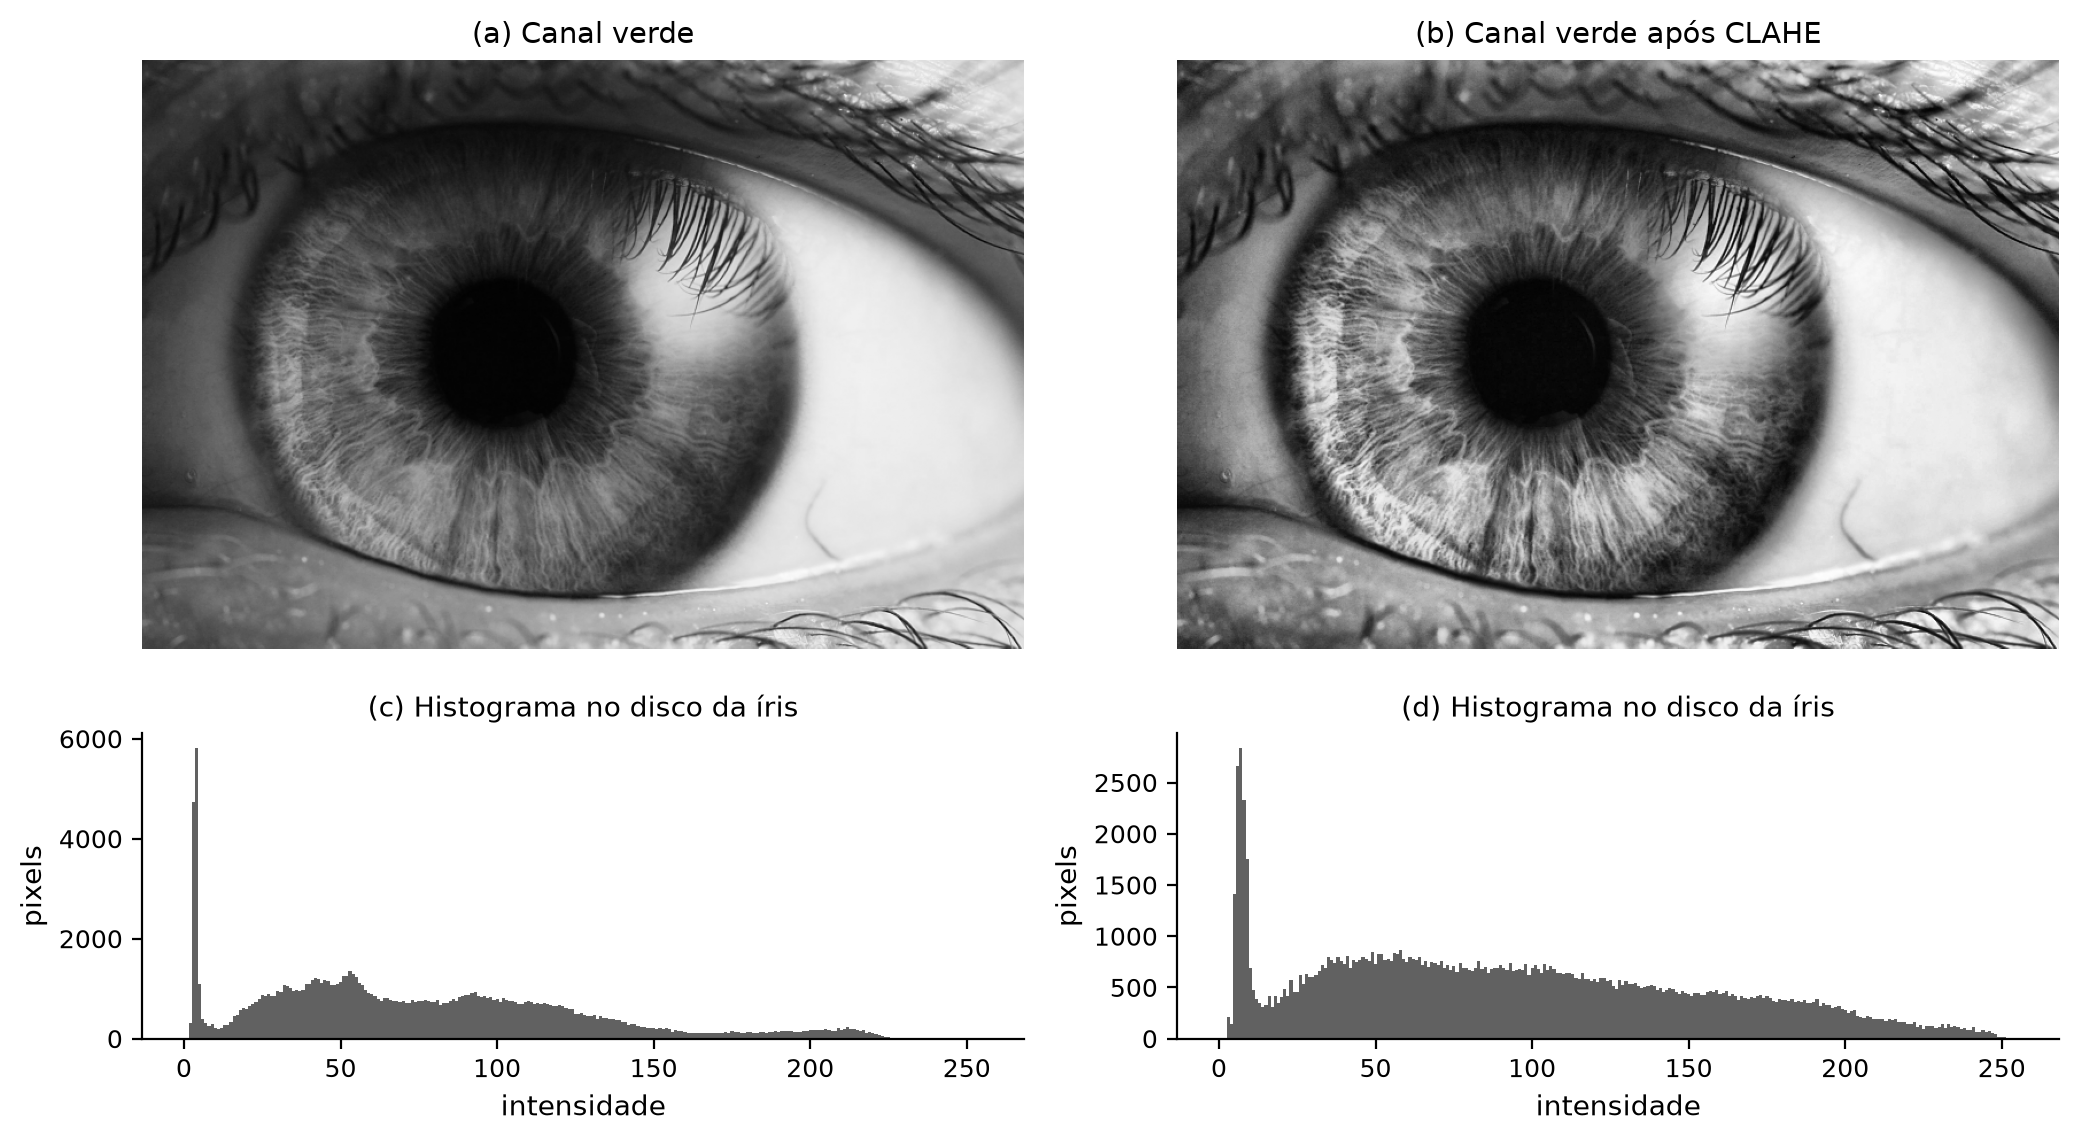
\includegraphics[width=0.95\textwidth]{clahe_novak.png}
  \fonte{Elaborada pelo autor (2026), a partir de fotografia de
  \citet{Novak2005}.}
\end{figure}

\begin{quadro}[htbp]
  \caption{Configuração padrão do pré-processamento, dos realces e da
  métrica}
  \label{qua:parametros}
  \footnotesize
  \renewcommand{\arraystretch}{1.15}
  \begin{tabular}{|l|l|>{\raggedright\arraybackslash}p{6.2cm}|}
    \hline
    \textbf{Etapa} & \textbf{Parâmetro} & \textbf{Valor} \\ \hline
    Redimensionamento & lado maior & 768 px (interpolação por área) \\ \hline
    Canal & entrada dos realces & verde (G) \\ \hline
    CLAHE & limite de recorte; grade & 2,0; $8 \times 8$ ladrilhos \\ \hline
    \multirow{4}{*}{Frangi} & escalas $\sigma$ & $\{1, 2, 3, 4\}$ \\ \cline{2-3}
     & $\beta$; $c$ & 0,5; 15 \\ \cline{2-3}
     & polaridade & cristas claras \\ \cline{2-3}
     & saída & recorte nos percentis 2 e 99, gama 0,7 \\ \hline
    \multirow{4}{*}{Gabor} & orientações $n$ & 8 (passo de $22{,}5^\circ$) \\ \cline{2-3}
     & $\lambda$; $\sigma$; $\gamma$; $\psi$ & 10; 4; 0,5; 0 \\ \cline{2-3}
     & núcleo & $21 \times 21$, média subtraída \\ \cline{2-3}
     & saída & máximo de $|$resposta$|$, normalização mínimo--máximo \\ \hline
    \multirow{2}{*}{Morfologia} & elementos estruturantes & elipses de 5, 11 e 21 px \\ \cline{2-3}
     & saída & soma \tht{} + \bh{}, normalização mínimo--máximo \\ \hline
    \multirow{2}{*}{Métrica} & limiar estrutura/fundo & Otsu sobre o mapa inteiro \\ \cline{2-3}
     & região das estatísticas & anel $\Omega$ (ou setor) \\ \hline
  \end{tabular}
  \fonte{Elaborado pelo autor (2026).}
\end{quadro}

\begin{figure}[htbp]
  \caption{Banco de filtros de Gabor utilizado no realce}
  \label{fig:gabor}
  \centering
  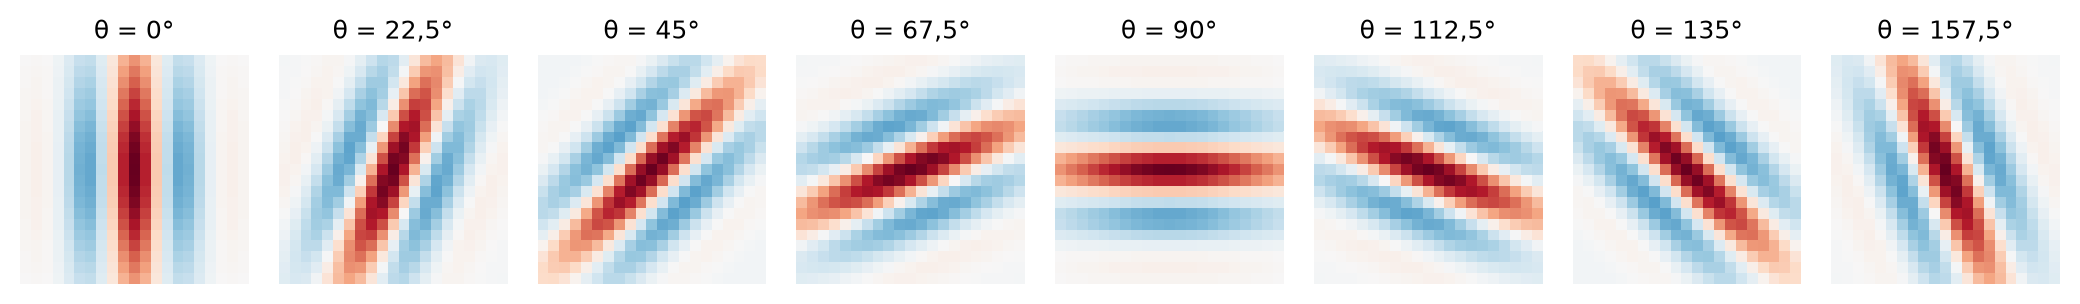
\includegraphics[width=\textwidth]{banco_gabor.png}
  \fonte{Elaborada pelo autor (2026).}
  \nota{Oito núcleos de $21 \times 21$ pixels, com $\lambda = 10$,
  $\sigma = 4$, $\gamma = 0{,}5$ e média subtraída.}
\end{figure}

\secao{Detecção da pupila e do limbo e região de medida}
\label{sec:met-deteccao}

A detecção empregada nesta etapa é deliberadamente simples e determinística
(Algoritmo~\ref{alg:deteccao}). A pupila é procurada como a região escura
mais circular e mais central da imagem, obtida por limiar no percentil 3 da
intensidade acrescido de 20 níveis, seguido de abertura e fechamento
morfológicos. O limbo é procurado pela transformada de Hough para círculos,
restrita a raios entre 1,6 e 6 vezes o raio da pupila e a centros próximos ao
da pupila. Quando uma etapa falha, o detector recorre a uma estimativa de
reserva e sinaliza esse fato; na macro da íris, em que o limbo não aparece, o
raio da íris é sempre estimado.

\begin{algorithm}[H]
  \caption{Detecção da pupila e do limbo}
  \label{alg:deteccao}
  \KwIn{imagem colorida $I$ (lado maior de 768 px), com $h \times w$ pixels}
  \KwOut{círculos $(\mathbf{c}_p, r_p)$ e $(\mathbf{c}_i, r_i)$; indicadores de estimativa}
  $g \leftarrow$ filtro de mediana $7 \times 7$ da imagem em tons de cinza\;
  $t \leftarrow$ percentil 3 de $g$ $+\,20$;\quad $D \leftarrow \{\mathbf{x} : g(\mathbf{x}) \le t\}$\;
  $D \leftarrow$ fechamento(abertura($D$, elipse $9 \times 9$), elipse $9 \times 9$, 2 iterações)\;
  \ForEach{contorno externo $C$ de $D$ com área $\ge 0{,}0015\,hw$}{
    $(\mathbf{c}, r) \leftarrow$ menor círculo que envolve $C$\;
    $\kappa \leftarrow \text{área}(C)/(\pi r^2)$;\quad $\eta \leftarrow 1 - \|\mathbf{c} - \mathbf{c}_{\mathrm{img}}\| / \|\mathbf{c}_{\mathrm{img}}\|$\;
    \If{$\kappa > 0{,}55$ \textbf{e} $\kappa + 0{,}5\,\eta$ é o maior até aqui}{
      $(\mathbf{c}_p, r_p) \leftarrow (\mathbf{c}, r)$\;
    }
  }
  \If{nenhum candidato}{
    $\mathbf{c}_p \leftarrow \arg\min g$;\quad $r_p \leftarrow 0{,}08\,\min(h,w)$;\quad pupila estimada\;
  }
  círculos $\leftarrow$ Hough($g$; $d_p = 1{,}2$; limiar de Canny 100; limiar do acumulador 40; $r \in [1{,}6\,r_p;\, 6\,r_p]$)\;
  $(\mathbf{c}_i, r_i) \leftarrow$ círculo com $\|\mathbf{c} - \mathbf{c}_p\| < 0{,}9\,r_p$ mais próximo de $\mathbf{c}_p$\;
  \If{nenhum círculo concêntrico}{
    $(\mathbf{c}_i, r_i) \leftarrow (\mathbf{c}_p,\; 0{,}48\,\min(h,w))$;\quad íris estimada\;
  }
  \Return{$(\mathbf{c}_p, r_p)$, $(\mathbf{c}_i, r_i)$ e os indicadores}\;
\end{algorithm}
\fonte{Elaborado pelo autor (2026).}

A região de medida é o anel $\Omega$, formado pelo disco do limbo excluído o
disco da pupila. Para a análise por regiões, $\Omega$ é dividido em 12 setores
angulares de $30^\circ$ centrados na pupila, numerados de S1 a S12 no sentido
anti-horário a partir da direita, com o eixo vertical da imagem orientado para
cima (Figura~\ref{fig:setores-layout}). A figura evidencia duas fontes de
contaminação do anel no olho completo: os cílios superiores sobrepostos à
íris nos setores S1 e S2 e a pálpebra superior, próxima ao limbo em S3 e S4.
Observa-se, ainda, que o círculo do limbo obtido pela transformada de Hough
está deslocado para a direita em relação ao limbo real e não cobre a íris em
S6 e S7, aspecto discutido na Seção~\ref{sec:res-pupila}.

\begin{figure}[htbp]
  \caption{Anel de medida e setores angulares no olho completo}
  \label{fig:setores-layout}
  \centering
  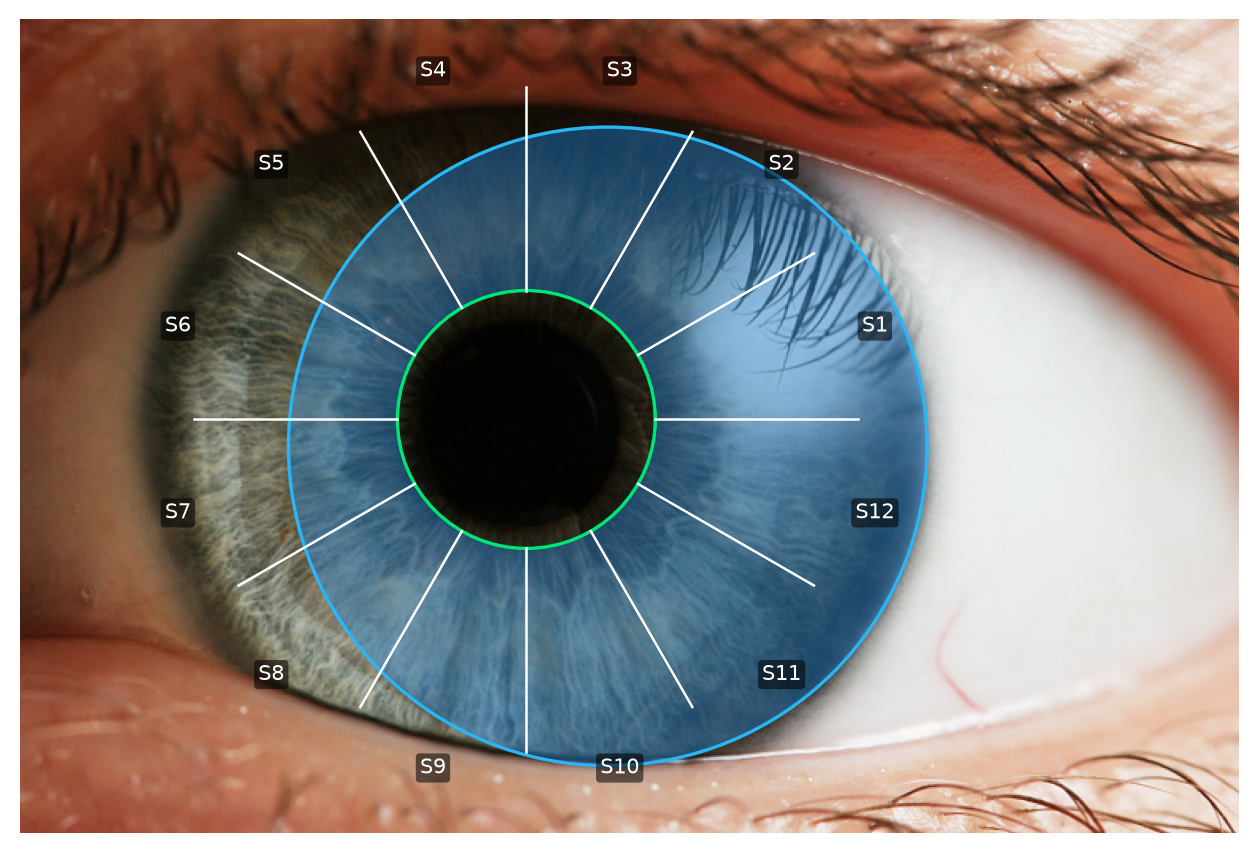
\includegraphics[width=0.78\textwidth]{setores_layout_novak.png}
  \fonte{Elaborada pelo autor (2026), a partir de fotografia de
  \citet{Novak2005}.}
  \nota{Pupila em verde, círculo do limbo em azul-claro e anel $\Omega$
  sombreado em azul.}
\end{figure}

\secao{Métricas e linhas de base}
\label{sec:met-metricas}

A métrica principal é a CNR da Equação~\eqref{eq:cnr}, calculada sobre o mapa
de 8 bits de cada método. A implementação
(\texttt{VascularizationEnhancer.quantify}) calcula o limiar de Otsu sobre
\emph{o mapa inteiro} e toma as estatísticas dentro do anel: os pixels de
$\Omega$ acima do limiar formam a estrutura, e os demais, o fundo. A escolha
do limiar global foi mantida por ser a adotada na cadeia de análise; o efeito
de restringir o limiar ao anel é medido no experimento E2. Quando a estrutura
ou o fundo ficam vazios em uma região, a CNR é indefinida e a região é
excluída da comparação correspondente. As medidas complementares são a
energia de cristas $E$, calculada em $\Omega$, e a entropia $H$ do histograma
em $\Omega$.

As linhas de base são as três operações disponíveis antes desta etapa: brilho
$+40$ e contraste $\times 1{,}8$ aplicados ao canal verde, e CLAHE. Em cada
comparação, o ganho de um realce é expresso em relação à \emph{melhor} linha
de base, isto é, àquela de maior valor na medida considerada, o que torna a
comparação conservadora.

\secao{Validador geométrico da pupila}
\label{sec:met-validador}

O validador (\texttt{PupilValidator}) recebe os raios e os centros da pupila
e do limbo e calcula três descritores adimensionais:
\begin{equation}
  \rho = \frac{r_p}{r_i},
  \qquad
  \tau = \frac{r_i - r_p}{r_i} = 1 - \rho,
  \qquad
  \epsilon = \frac{\|\mathbf{c}_p - \mathbf{c}_i\|}{r_i}.
  \label{eq:descritores}
\end{equation}
A razão $\rho$ mede a dilatação relativa da pupila, $\tau$ a largura radial do
anel e $\epsilon$ a excentricidade entre os centros. Como $\tau = 1 - \rho$, o
critério de espessura equivale a um limite superior adicional para $\rho$; ele
é mantido separado por comunicar um motivo diferente, a saber, um anel
estreito demais para a extração de textura. O validador registra ainda os
diâmetros e a espessura em pixels e, quando há escala conhecida, em
milímetros. A classificação segue o Algoritmo~\ref{alg:validador}, com as
faixas do Quadro~\ref{qua:faixas}.

\begin{algorithm}[H]
  \caption{Validação geométrica da pupila}
  \label{alg:validador}
  \KwIn{raios $r_p, r_i$ e centros $\mathbf{c}_p, \mathbf{c}_i$}
  \KwOut{rótulo, pontuação $q$ e lista de motivos $M$}
  \lIf{$r_p \le 0$ \textbf{ou} $r_i \le r_p$}{\Return{\texttt{invalid} com o motivo}}
  calcular $\rho$, $\tau$ e $\epsilon$ (Equação~\ref{eq:descritores});\quad $q \leftarrow 1$;\quad $M \leftarrow \emptyset$\;
  \uIf{$\rho \notin [0{,}15;\, 0{,}80]$}{
    $q \leftarrow q - 0{,}6$;\quad acrescentar a $M$: fora da faixa plausível (falha grave)\;
  }
  \ElseIf{$\rho \notin [0{,}20;\, 0{,}70]$}{
    $q \leftarrow q - 0{,}25$;\quad acrescentar a $M$: faixa de atenção\;
  }
  \lIf{$\tau < 0{,}25$}{$q \leftarrow q - 0{,}3$;\quad acrescentar a $M$: anel fino demais}
  \lIf{$\epsilon > 0{,}30$}{$q \leftarrow q - 0{,}3$;\quad acrescentar a $M$: centros pouco concêntricos}
  $q \leftarrow \min(1, \max(0, q))$\;
  \uIf{falha grave \textbf{ou} $q < 0{,}5$}{rótulo $\leftarrow$ \texttt{invalid}\;}
  \uElseIf{$q < 0{,}8$ \textbf{ou} $M \neq \emptyset$}{rótulo $\leftarrow$ \texttt{borderline}\;}
  \lElse{rótulo $\leftarrow$ \texttt{valid}}
  \Return{rótulo, $q$, $M$}\;
\end{algorithm}
\fonte{Elaborado pelo autor (2026).}

\begin{quadro}[htbp]
  \caption{Faixas do validador geométrico e sua origem}
  \label{qua:faixas}
  \footnotesize
  \renewcommand{\arraystretch}{1.15}
  \begin{tabular}{|>{\raggedright\arraybackslash}p{3.2cm}
                  |>{\raggedright\arraybackslash}p{2.4cm}
                  |>{\raggedright\arraybackslash}p{8.3cm}|}
    \hline
    \textbf{Critério} & \textbf{Valor} & \textbf{Origem} \\ \hline
    Faixa normal de $\rho$ & $[0{,}20;\, 0{,}70]$ & Arredondamento do
      intervalo $[0{,}17;\, 0{,}68]$, obtido de pupila entre 2 e 8~mm
      \citep*{WatsonYellott2012} e de íris de 11,71~mm \citep*{Rufer2005}. \\ \hline
    Faixa plausível de $\rho$ & $[0{,}15;\, 0{,}80]$ & Margem para variação
      individual do diâmetro da íris, miose e midríase farmacológica e erro
      de segmentação; fora dela, a geometria é considerada implausível. \\ \hline
    Espessura mínima $\tau$ & 0,25 & Anel com largura de pelo menos um
      quarto do raio da íris, o que equivale a $\rho \le 0{,}75$. \\ \hline
    Excentricidade máxima $\epsilon$ & 0,30 & Tolerância heurística para o
      deslocamento entre os centros, sem referência fisiológica verificada
      nesta etapa. \\ \hline
    Penalidades e rótulos & 0,6; 0,25; 0,3; 0,3; limiares 0,5 e 0,8 &
      Escolhas de projeto: uma violação leve isolada produz
      \texttt{borderline}; uma violação grave ou duas violações produzem
      \texttt{invalid}. Os valores não foram ajustados a dados. \\ \hline
  \end{tabular}
  \fonte{Elaborado pelo autor (2026).}
\end{quadro}

Os rótulos \texttt{valid}, \texttt{borderline} e \texttt{invalid}
correspondem, respectivamente, a geometria válida, limítrofe (aceitável com
ressalva) e inválida. Os seis valores calculados (diâmetros, espessura, $\rho$,
$\tau$ e $\epsilon$) também formam um vetor de descritores apto a alimentar um
classificador supervisionado quando houver dados rotulados, o que permitiria
aprender os limiares em vez de fixá-los. Para uma estimativa de ordem de
grandeza em milímetros, quando a escala da imagem não é conhecida, utiliza-se o
diâmetro médio da íris como referência: $\text{px/mm} = D_i/11{,}71$
\citep*{Rufer2005}.

\secao{Desenho experimental}
\label{sec:met-experimentos}

O Quadro~\ref{qua:experimentos} resume os onze experimentos. Os detalhes que
não decorrem diretamente das seções anteriores são descritos nas subseções
seguintes.

\begin{quadro}[htbp]
  \caption{Experimentos realizados, perguntas a que respondem e medidas
  empregadas}
  \label{qua:experimentos}
  \footnotesize
  \renewcommand{\arraystretch}{1.12}
  \begin{tabular}{|>{\raggedright\arraybackslash}p{2.5cm}
                  |>{\raggedright\arraybackslash}p{4.4cm}
                  |>{\raggedright\arraybackslash}p{3.3cm}
                  |>{\raggedright\arraybackslash}p{3.6cm}|}
    \hline
    \textbf{Experimento} & \textbf{Pergunta} & \textbf{Dados} &
      \textbf{Medidas} \\ \hline
    E0 Comparação principal & Os realces superam as linhas de base? &
      2 imagens reais & CNR, $E$, $H$ \\ \hline
    E1 Setores angulares & O ganho é consistente ao longo da íris? &
      24 setores de $30^\circ$ & CNR; Wilcoxon; \emph{bootstrap} \\ \hline
    E2 Limiar da métrica & A conclusão depende da região de cálculo do
      limiar? & 2 imagens & CNR com Otsu global e no anel \\ \hline
    E3 Escalas do Frangi & Que escala domina e qual o efeito da normalização
      de saída? & 2 imagens & dominância, resposta média, CNR \\ \hline
    E4 Sensibilidade & Quão dependentes dos parâmetros são os resultados? &
      2 imagens, 29 configurações & CNR \\ \hline
    E5 Robustez & Os mapas mudam sob perturbações de aquisição? & 2 imagens,
      9 perturbações & $r$ de Pearson, Dice, retenção da CNR \\ \hline
    E6 Fantoma & A CNR concorda com uma verdade de referência? &
      50 fantomas (5 níveis de ruído, 10 sementes) & AUC, CNR com verdade,
      CNR por Otsu, Spearman \\ \hline
    E7 Custo & Quanto tempo cada etapa demanda? & imagem de $768 \times 513$
      px & mediana de 7 execuções \\ \hline
    E8 Normalização polar & Como as estruturas se distribuem no raio? &
      2 imagens & densidade de estrutura por raio \\ \hline
    E9 Validação da pupila & O validador e a detecção são confiáveis? &
      imagem real, 7 casos sintéticos, 15 condições & $\rho$, $\tau$,
      $\epsilon$, rótulo \\ \hline
    E10 Canal de cor & O canal verde é a melhor entrada? & 2 imagens,
      4 canais & CNR \\ \hline
  \end{tabular}
  \fonte{Elaborado pelo autor (2026).}
\end{quadro}

\subsection{Análise por setores angulares (E1)}

Em cada setor, a CNR de cada método é calculada com o mesmo protocolo da
medida global, e cada realce é comparado com a melhor linha de base
\emph{daquele setor}. Emprega-se o teste de Wilcoxon pareado unilateral, cuja
hipótese alternativa é a de que o realce apresenta CNR maior, aplicado às
diferenças; a razão mediana entre a CNR do realce e a da melhor linha de base
recebe um intervalo de confiança de 95\% por \emph{bootstrap} percentil com
10.000 reamostragens (semente 0). Setores com menos de 500 pixels seriam
descartados, o que não ocorreu. Como os setores de uma mesma imagem são
vizinhos e compartilham a iluminação, eles não constituem observações
independentes; os valores-$p$ descrevem a consistência do efeito dentro de
cada imagem, e não a generalização para outras íris. Uma análise de
sensibilidade exclui os setores S1 e S2 do olho completo, contaminados pelos
cílios.

\subsection{Fantoma sintético (E6)}
\label{sec:met-fantoma}

Cada fantoma possui $384 \times 384$ pixels e resulta da soma de quatro
componentes: (i) iluminação não uniforme, dada por
$70 + 50\,x/384 + 25\cos(\pi y/384)$; (ii) textura de fundo, formada por ruído
gaussiano suavizado ($\sigma = 6$) e reescalado para desvio-padrão 12;
(iii) 28 estruturas tubulares claras, desenhadas como curvas de Bézier
quadráticas com pontos de controle aleatórios, largura de 1, 2 ou 3 pixels e
contraste uniforme entre 12 e 35 níveis, suavizadas por uma gaussiana de
$\sigma = 0{,}7$; e (iv) ruído gaussiano branco com desvio-padrão
$\sigma_n \in \{4, 8, 12, 16, 24\}$. A verdade de referência é a máscara das
curvas antes da suavização, que ocupa 15,2\% do campo de visão na semente 0.
Para cada nível de ruído, geram-se 10 fantomas (sementes 0 a 9), e as medidas
excluem uma borda de 12 pixels. Os métodos são aplicados exatamente como nas
imagens reais. Além da AUC, calculam-se a CNR com a verdade de referência, na
qual estrutura e fundo são definidos pela máscara verdadeira, e a CNR por
Otsu, a mesma empregada nas imagens reais. A correlação de Spearman entre a
CNR por Otsu e a AUC, nas 35 combinações de ruído e método, indica se a
métrica sem verdade de referência ordena os métodos da mesma forma que a
métrica com verdade.

\subsection{Perturbações (E5 e E9)}

As nove perturbações são: brilho $\pm 30$, com saturação em 0 e 255;
contraste $\times 0{,}7$ e $\times 1{,}3$; correção gama 0,7 e 1,5; ruído
gaussiano ($\sigma = 8$, semente 0); desfoque gaussiano ($\sigma = 1{,}5$); e
compressão JPEG com qualidade 30. Elas são aplicadas à imagem colorida antes
de todo o processamento. No E5, a região $\Omega$ é a da imagem original, de
modo a isolar o efeito sobre o realce, e medem-se a correlação de Pearson
entre os mapas em $\Omega$, o coeficiente de Dice entre as máscaras de
estrutura e a razão entre a CNR após e antes da perturbação. No E9, a detecção
e a validação são refeitas em cada condição; às perturbações somam-se três
mudanças de escala (lado maior de 384, 576 e 1152 pixels a partir do
original), uma rotação de $10^\circ$ e um espelhamento horizontal.

\subsection{Demais experimentos}

No E3, as respostas do filtro de Frangi em cada escala são calculadas
separadamente; a dominância de uma escala é a fração dos pixels de estrutura
em que ela produz a maior resposta, e verifica-se se o máximo das respostas
individuais coincide com a saída multiescala. Avaliam-se também três
normalizações de saída do mapa de Frangi. No E4, cada parâmetro é variado
isoladamente em torno da configuração padrão, em 29 configurações; na
varredura de $\sigma$ do filtro de Gabor, o núcleo cresce para
$\max(21, 2\lceil 2{,}5\sigma\rceil + 1)$ pixels, de modo a cobrir a
envoltória. No E7, cada etapa é executada uma vez para aquecimento e, em
seguida, sete vezes, em um único processo, registrando-se mediana, mínimo e
máximo. No E8, o anel é desdobrado pela Equação~\eqref{eq:rubber} em 64
amostras radiais e 720 angulares, com interpolação bilinear, e calcula-se a
fração de pixels de estrutura do mapa de Frangi em cada raio. No E10, cada
canal (R, G, B e a luminância $Y = 0{,}299R + 0{,}587G + 0{,}114B$) é
replicado e submetido ao mesmo processamento.

\secao{Reprodutibilidade e testes}

Todos os resultados das Seções~\ref{cap:resultados} e~\ref{cap:discussao} são
produzidos por \arq{experiments/report_experiments.py}, que grava as figuras
em \arq{docs/PGC_2/figuras}, as tabelas em \arq{docs/PGC_2/tabelas},
incluídas neste documento sem edição manual, as séries dos gráficos em
\arq{docs/PGC_2/dados} e um resumo completo em
\arq{results/report/resumo.json}. As sementes são fixas, e as versões das
bibliotecas empregadas
\citep*{Bradski2000,Harris2020,Hunter2007,Pedregosa2011,vanderWalt2014,Virtanen2020}
constam do Apêndice~\ref{ap:repro}. O módulo de testes
\arq{tests/test_vascularization_and_pupil.py} contém onze testes unitários:
cinco para o realce (formato e faixa das saídas, entrada em tons de cinza,
métricas, vantagem do filtro de Frangi sobre o brilho em uma estrutura
sintética e imagem constante) e seis para o validador (geometria normal,
dilatação e constrição excessivas, excentricidade, íris menor que a pupila e
vetor de descritores).

\secao{Aspectos éticos e licenças}

As duas fotografias são públicas, com licenças Creative Commons que permitem
o uso com atribuição, e não estão associadas a dados de saúde. Nenhum dado
pessoal ou clínico foi coletado nesta etapa. As imagens são utilizadas apenas
para ilustrar e verificar os métodos, e nenhum resultado deste relatório deve
ser interpretado como diagnóstico ou como evidência sobre o DM2.

% ============================================================================
\chapter{Resultados}
\label{cap:resultados}

Os resultados a seguir foram produzidos em uma única execução do
\emph{script} de experimentos, no ambiente descrito no
Apêndice~\ref{ap:repro}. Os números decimais são apresentados com vírgula e,
nas tabelas, o melhor resultado de cada bloco aparece em negrito quando a
comparação é direta.

\secao{Comparação principal (E0)}
\label{sec:res-principal}

A Tabela~\ref{tab:vasc-principal} compara as linhas de base e os três realces
no anel da íris, e a Figura~\ref{fig:barras-cnr} resume a CNR. O filtro de
Frangi obteve a maior CNR nas duas imagens: 8,24 no olho completo e 7,29 na
macro da íris, contra 3,49 e 3,62 da melhor linha de base (contraste
$\times 1{,}8$ nos dois casos), o que corresponde a razões de 2,36 e 2,02. A
energia de cristas do filtro de Frangi correspondeu a 5,25 e 5,33 vezes a da
melhor linha de base. O banco de Gabor também superou as linhas de base em
CNR (5,90 e 4,31, isto é, 1,69 e 1,19 vez a melhor linha de base), porém com
energia de cristas menor, uma vez que sua resposta é suave. O realce \bh{}
apresentou ganho apenas no olho completo (4,38, ou 1,25 vez) e permaneceu no
nível da linha de base na macro da íris (3,56, ou 0,98 vez).

\begin{table}[htbp]
  \caption{Visibilidade das estruturas no anel da íris (E0)}
  \label{tab:vasc-principal}
  \centering\footnotesize
  % Gerado por experiments/report_experiments.py (não editar à mão).
\begin{tabular}{llccccc}
\toprule
Imagem & Método & CNR & $E$ & $H$ (bits) & CNR ($\times$base) & $E$ ($\times$base) \\
\midrule
\multirow{7}{*}{Olho completo} & Original (verde) & 3,22 & 0,080 & 7,37 & 0,92 & 0,49 \\
 & Brilho $+40$ (base) & 3,21 & 0,079 & 7,33 & 0,92 & 0,48 \\
 & Contraste $\times1{,}8$ (base) & 3,49 & 0,165 & 6,60 & 1,00 & 1,00 \\
 & CLAHE (base) & 3,26 & 0,164 & 7,73 & 0,93 & 0,99 \\
 & \textbf{Frangi} & \textbf{8,24} & \textbf{0,866} & \textbf{4,80} & \textbf{2,36} & \textbf{5,25} \\
 & Gabor & 5,90 & 0,046 & 5,75 & 1,69 & 0,28 \\
 & \textit{Black-hat} & 4,38 & 0,023 & 6,57 & 1,25 & 0,14 \\
\midrule
\multirow{7}{*}{Macro da íris} & Original (verde) & 3,54 & 0,028 & 7,20 & 0,98 & 0,27 \\
 & Brilho $+40$ (base) & 3,54 & 0,028 & 7,20 & 0,98 & 0,27 \\
 & Contraste $\times1{,}8$ (base) & 3,62 & 0,080 & 6,23 & 1,00 & 0,78 \\
 & CLAHE (base) & 3,34 & 0,103 & 7,77 & 0,92 & 1,00 \\
 & \textbf{Frangi} & \textbf{7,29} & \textbf{0,549} & \textbf{5,06} & \textbf{2,02} & \textbf{5,33} \\
 & Gabor & 4,31 & 0,137 & 6,82 & 1,19 & 1,33 \\
 & \textit{Black-hat} & 3,56 & 0,049 & 7,01 & 0,98 & 0,48 \\
\bottomrule
\end{tabular}

  \fonte{Elaborada pelo autor (2026).}
  \nota{CNR: razão contraste-ruído; $E$: energia de cristas; $H$: entropia.
  As colunas ``$\times$base'' dividem cada valor pelo da melhor linha de base
  na mesma medida.}
\end{table}

\begin{figure}[htbp]
  \caption{CNR no anel da íris por método nas duas imagens (E0)}
  \label{fig:barras-cnr}
  \centering
  \begin{tikzpicture}
    \begin{axis}[
      width=0.95\textwidth, height=6.3cm,
      ybar, bar width=10pt,
      ymin=0, ymax=10.6, ytick={0,2,...,10},
      ylabel={CNR no anel $\Omega$},
      xtick=data,
      xticklabels={Original, {Brilho\\$+40$}, {Contraste\\$\times1{,}8$}, CLAHE,
                   Frangi, Gabor, \emph{Black-hat}},
      x tick label style={font=\small, align=center},
      enlarge x limits=0.08,
      ymajorgrids, grid style={gray!25},
      legend style={at={(0.02,0.97)}, anchor=north west, font=\small,
                    draw=none, fill=white, fill opacity=0.8, text opacity=1},
      legend cell align=left,
      nodes near coords={\pgfmathprintnumber[fixed, fixed zerofill,
                         precision=2]{\pgfplotspointmeta}},
      every node near coord/.append style={font=\scriptsize, rotate=90,
                                           anchor=west}]
      \addplot[fill=blue!55, draw=blue!70!black]
        table[x expr=\coordindex, y=novak] {dados/cnr_principal.dat};
      \addplot[fill=orange!60, draw=orange!70!black]
        table[x expr=\coordindex, y=closeup] {dados/cnr_principal.dat};
      \legend{Olho completo, Macro da íris}
    \end{axis}
  \end{tikzpicture}
  \fonte{Elaborada pelo autor (2026).}
\end{figure}

As linhas de base comportaram-se conforme previsto pela Proposição~1. O
brilho $+40$ produziu praticamente a mesma CNR do canal original (3,21 contra
3,22 no olho completo; 3,54 contra 3,54 na macro), e as pequenas diferenças
decorrem da saturação de pixels claros da esclera e de reflexos em 255. O
contraste $\times 1{,}8$ elevou a CNR para 3,49 e 3,62; como uma
transformação afim sem saturação manteria a CNR inalterada, esse aumento
deve-se inteiramente à saturação, visível como o pico em 255 no histograma
da Figura~\ref{fig:histograma}. Trata-se de perda de informação nos tons
claros, e não de ganho estrutural. O mesmo histograma exibe o padrão em pente
produzido pelo contraste, uma vez que a transformação apenas redistribui os
256 níveis originais e deixa lacunas entre eles. A CLAHE apresentou CNR
próxima à do original (3,26 e 3,34), mas aproximadamente duplicou a energia
de cristas no olho completo, o que ilustra que ela amplifica detalhes de
qualquer natureza sem separar estruturas do fundo.

\begin{figure}[htbp]
  \caption{Histogramas de estrutura e de fundo no anel do olho completo para
  o contraste $\times 1{,}8$ e para o filtro de Frangi (E0)}
  \label{fig:histograma}
  \centering
  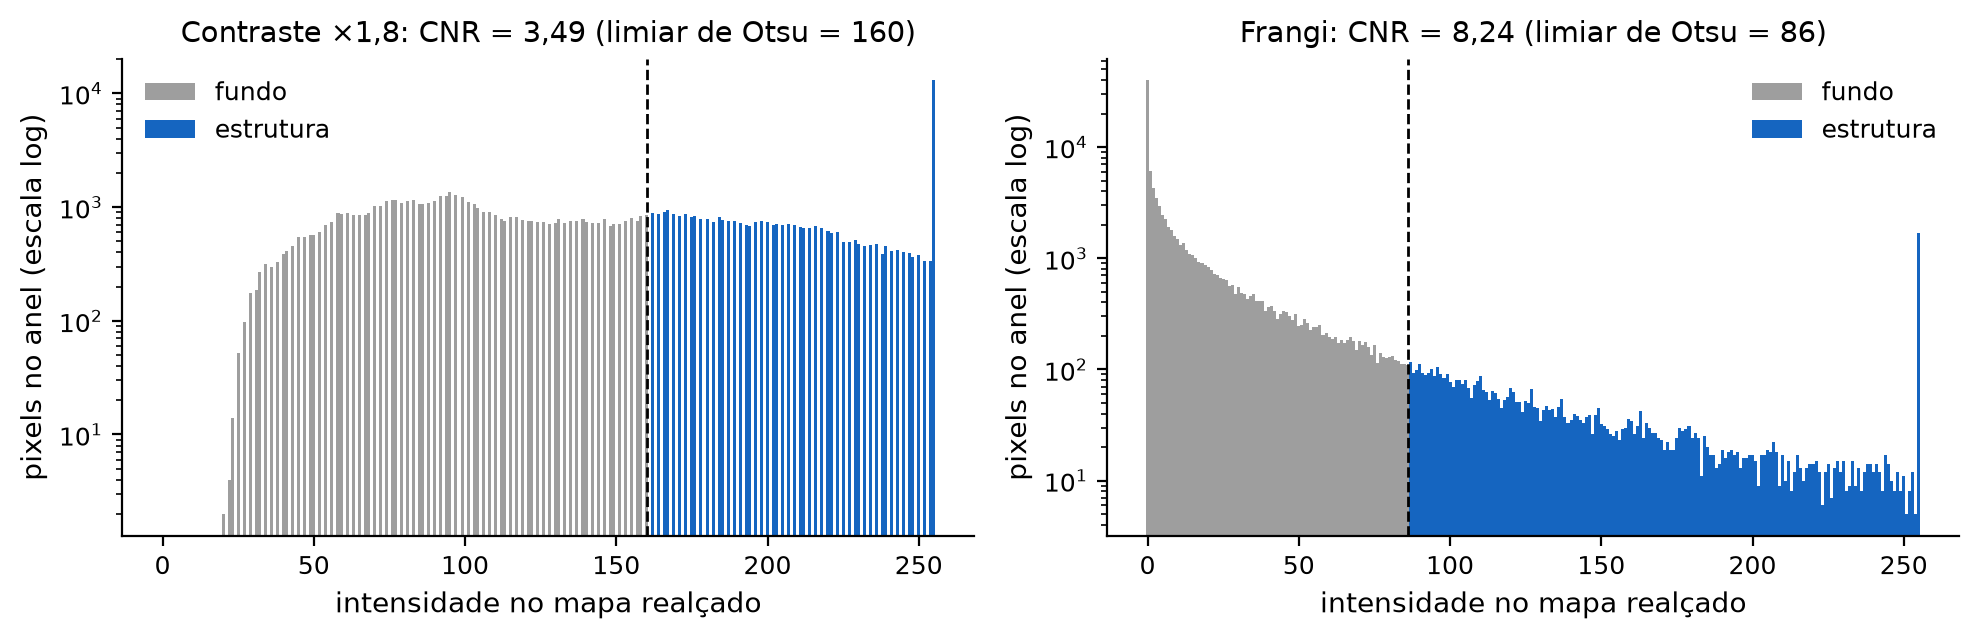
\includegraphics[width=\textwidth]{histograma_estrutura_fundo.png}
  \fonte{Elaborada pelo autor (2026), a partir de fotografia de
  \citet{Novak2005}.}
  \nota{Escala logarítmica; a linha tracejada indica o limiar de Otsu.}
\end{figure}

A entropia diminuiu nos três realces, passando de 7,37 bits no original para
4,80 no filtro de Frangi, no olho completo. Esse resultado é esperado para
mapas esparsos e mostra por que a entropia não serve como medida de qualidade
do realce neste problema: um mapa que anula o fundo e preserva apenas as
estruturas ocupa poucos níveis de cinza. As Figuras~\ref{fig:painel-novak}
e~\ref{fig:painel-closeup} apresentam a comparação visual, e a
Figura~\ref{fig:detalhe} amplia um trecho do estroma da macro da íris. No
olho completo, o filtro de Frangi exibe as fibras radiais como linhas finas
sobre fundo escuro, e a região superior direita, com resposta intensa nos três
realces, corresponde aos cílios sobrepostos à íris. Na macro, o filtro de
Frangi isola as trabéculas radiais, o banco de Gabor produz uma resposta mais
contínua e orientada e o realce \bh{} destaca regiões mais largas, incluindo
bordas de criptas. No detalhe ampliado, o contraste $\times 1{,}8$ satura as
regiões claras, ao passo que o filtro de Frangi delineia fibras e bordas de
criptas como linhas finas e o banco de Gabor responde às fibras com faixas
suaves e contínuas.

\begin{figure}[htbp]
  \caption{Comparação visual entre o canal original, as linhas de base e os
  realces no olho completo (E0)}
  \label{fig:painel-novak}
  \centering
  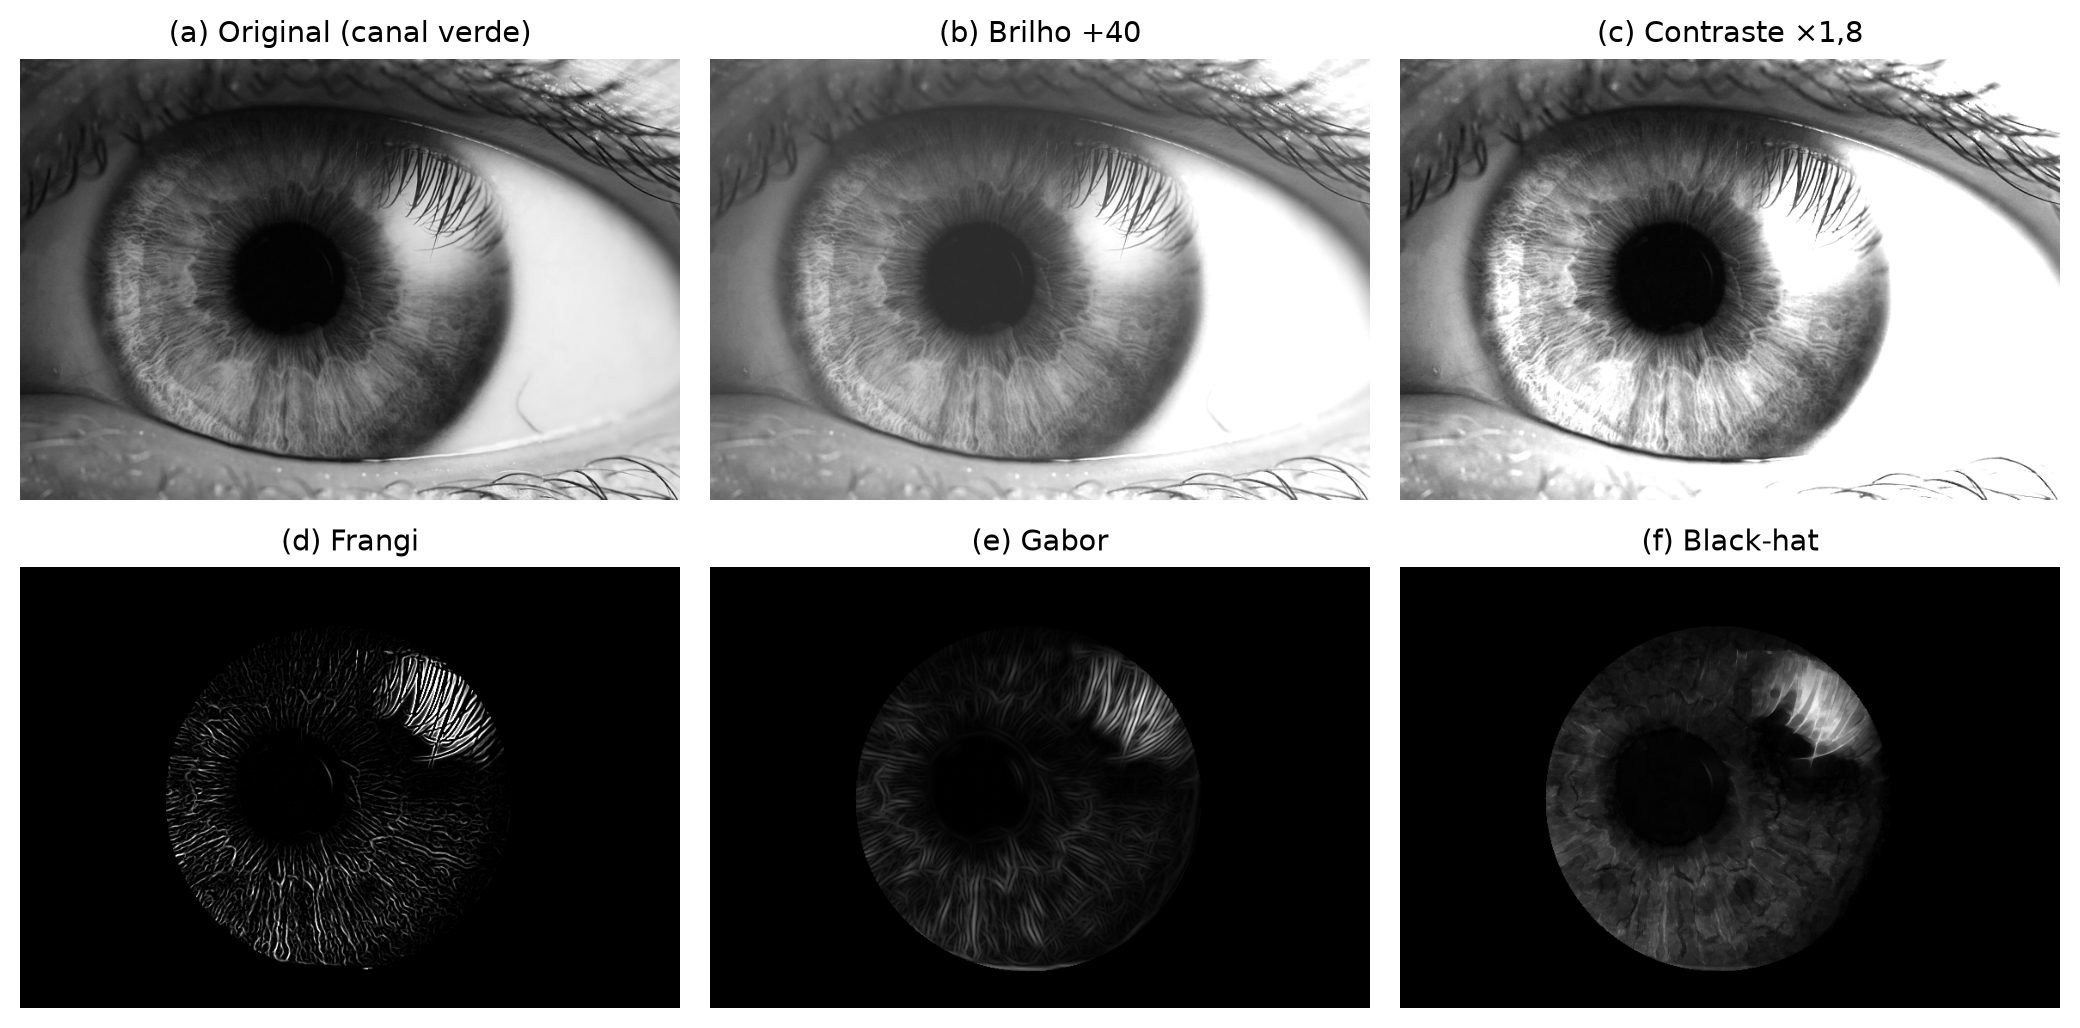
\includegraphics[width=\textwidth]{painel_vascularizacao_novak.png}
  \fonte{Elaborada pelo autor (2026), a partir de fotografia de
  \citet{Novak2005}.}
  \nota{Os mapas de realce (d a f) estão restritos ao disco da íris
  detectado.}
\end{figure}

\begin{figure}[htbp]
  \caption{Comparação visual entre o canal original, as linhas de base e os
  realces na macro da íris (E0)}
  \label{fig:painel-closeup}
  \centering
  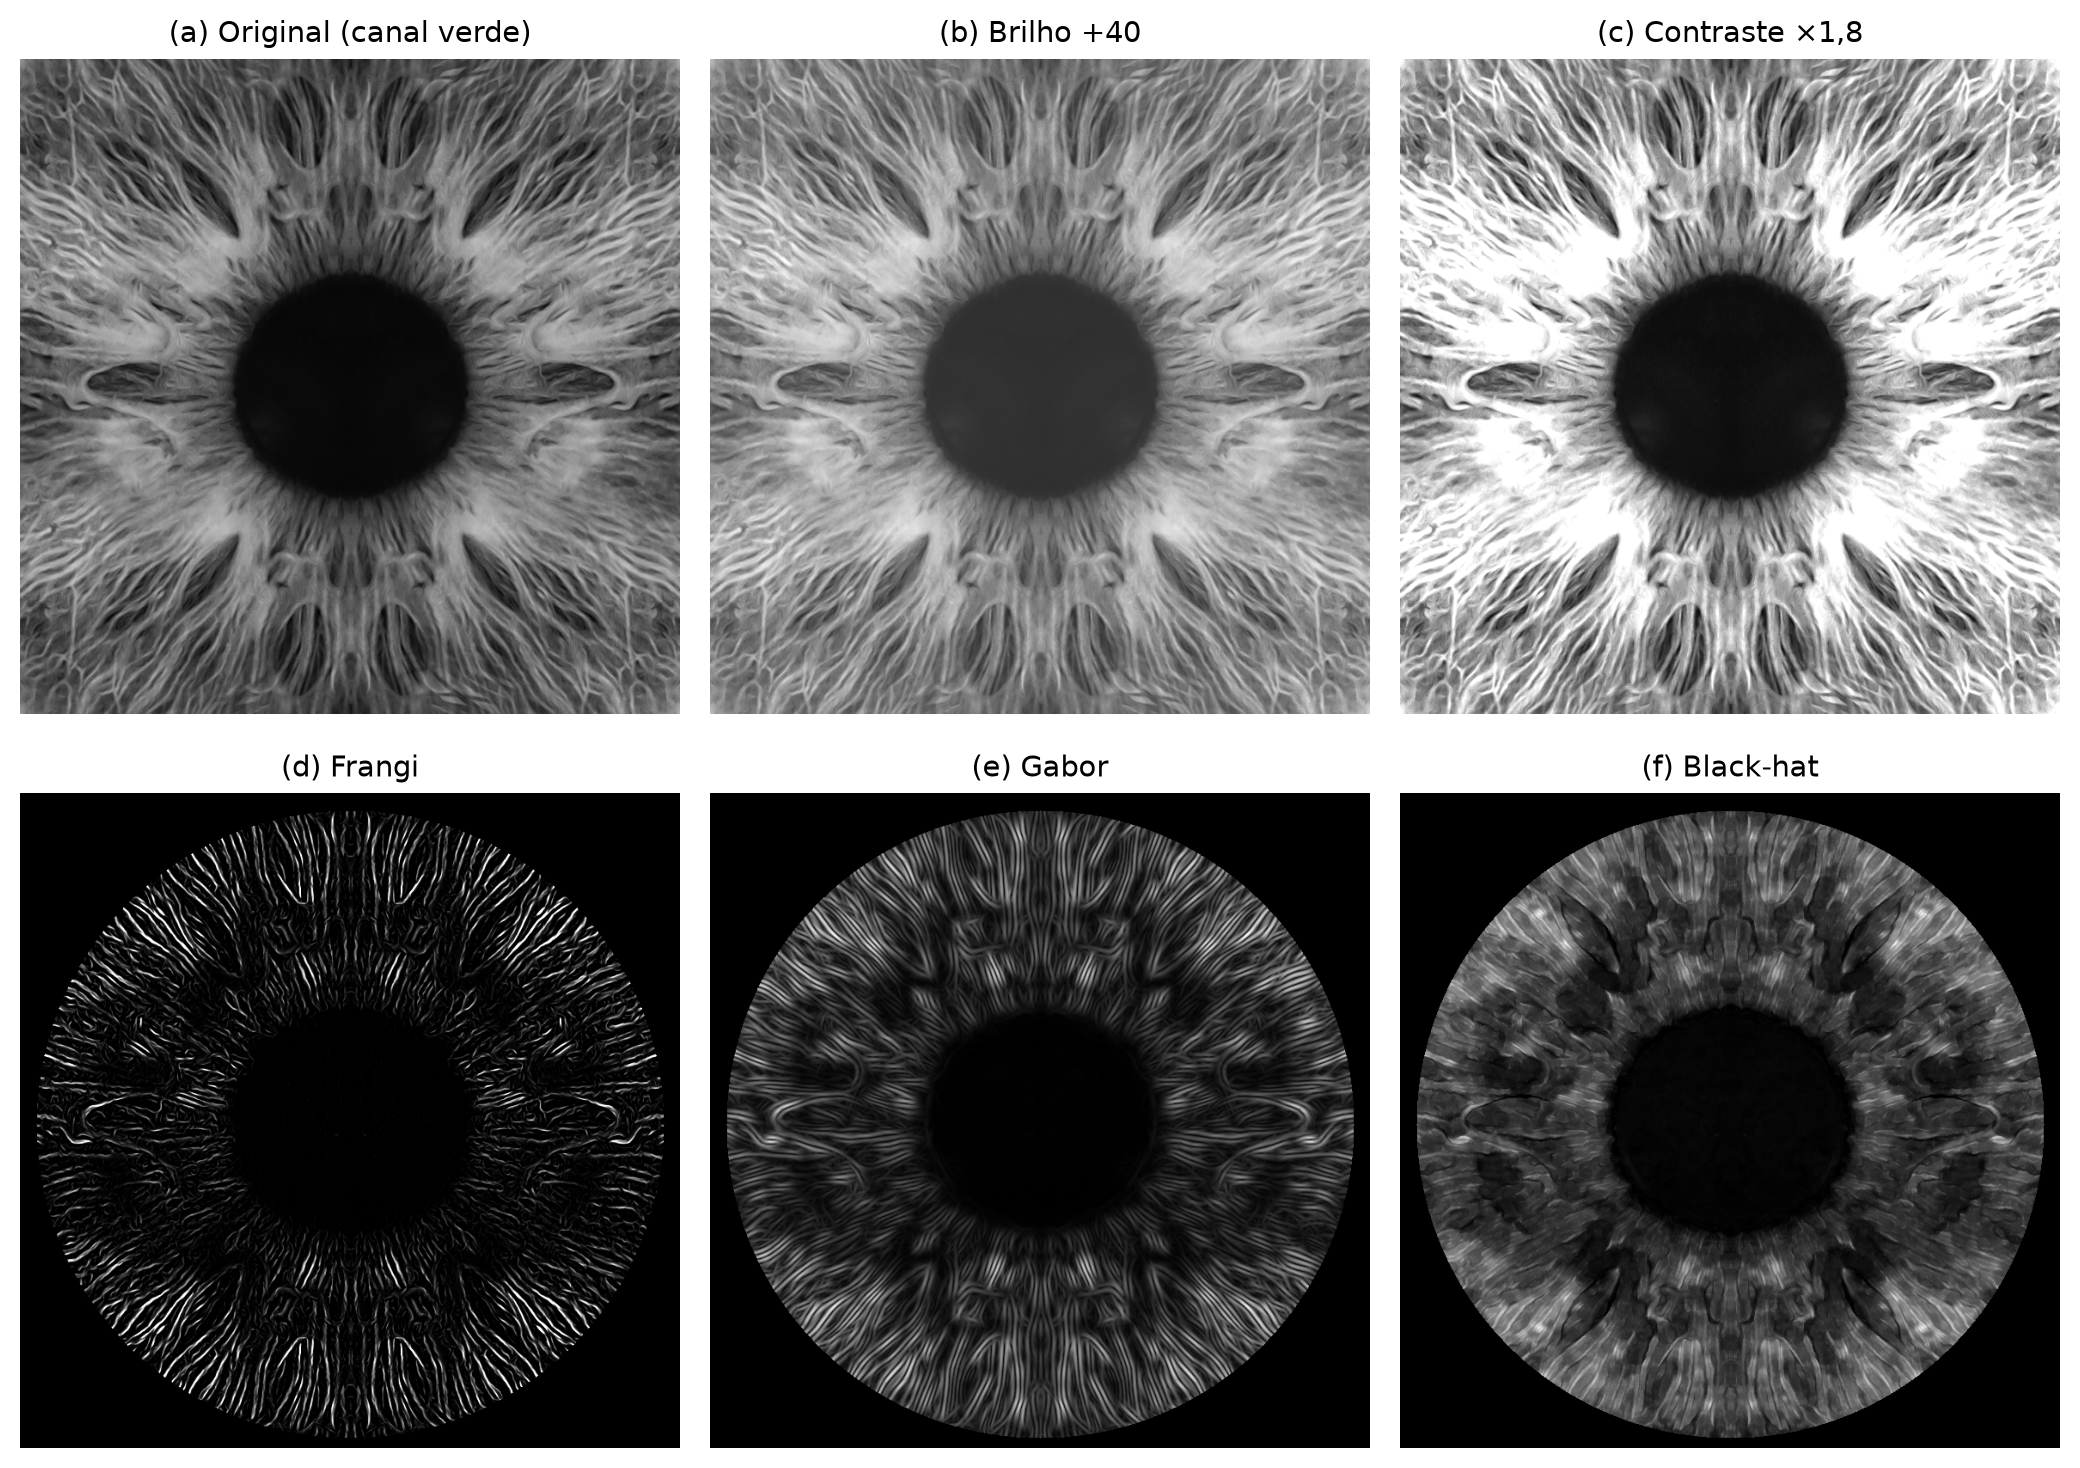
\includegraphics[width=\textwidth]{painel_vascularizacao_closeup.png}
  \fonte{Elaborada pelo autor (2026), a partir de fotografia de
  \citet{Reyes2014}.}
\end{figure}

\begin{figure}[htbp]
  \caption{Detalhe ampliado de um trecho de $124 \times 124$ pixels do
  estroma da macro da íris (E0)}
  \label{fig:detalhe}
  \centering
  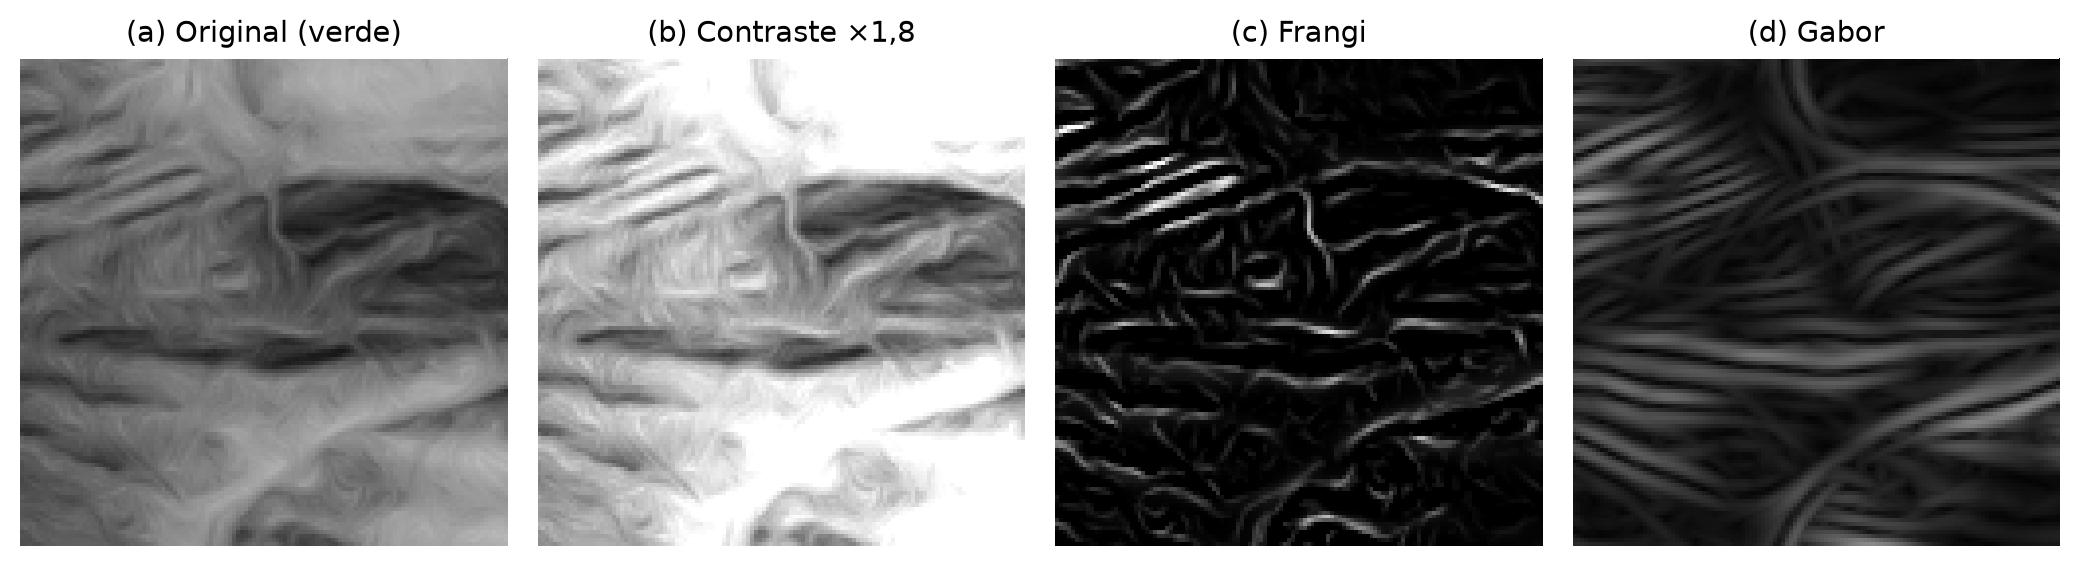
\includegraphics[width=\textwidth]{detalhe_estroma_closeup.png}
  \fonte{Elaborada pelo autor (2026), a partir de fotografia de
  \citet{Reyes2014}.}
\end{figure}

\secao{Consistência por setores angulares (E1)}
\label{sec:res-setores}

A Tabela~\ref{tab:setores} resume a comparação por setores. O filtro de
Frangi superou a melhor linha de base do setor em todos os 24 setores, com
razão mediana de 1,85 (IC~95\%: 1,55 a 2,68) no olho completo e de 2,01
(IC~95\%: 1,61 a 2,21) na macro da íris; nos dois conjuntos reunidos, a razão
mediana foi de 1,92 (IC~95\%: 1,64 a 2,23), com $p < 0{,}001$. O banco de
Gabor superou a linha de base em 8 de 11 setores do olho completo e em 9 de 12
da macro, com razões medianas de 1,21 e 1,14; no conjunto, superou-a em 17 de
23 setores ($p < 0{,}001$), com intervalo de confiança da razão acima de 1
(1,03 a 1,34). O realce \bh{} não apresentou ganho consistente: superou a
linha de base em 5 de 12 e em 4 de 12 setores, com razões medianas de 0,96 e
0,99 e valores-$p$ de 0,339 e 0,849.

\begin{table}[htbp]
  \caption{Comparação por setores angulares de $30^\circ$ (E1)}
  \label{tab:setores}
  \centering\footnotesize
  \setlength{\tabcolsep}{4pt}
  % Gerado por experiments/report_experiments.py (não editar à mão).
\begin{tabular}{llccccc}
\toprule
Conjunto & Algoritmo & $n$ & Mediana CNR & Razão mediana (IC 95\%) & Vitórias & $p$ (Wilcoxon) \\
\midrule
\multirow{3}{*}{Olho completo} & Frangi & 12 & 6,16 & 1,85 (1,55--2,68) & 12/12 & $<0{,}001$ \\
 & Gabor & 11 & 3,65 & 1,21 (0,98--1,60) & 8/11 & 0,021 \\
 & \textit{Black-hat} & 12 & 2,96 & 0,96 (0,75--1,86) & 5/12 & 0,339 \\
\midrule
\multirow{3}{*}{Macro da íris} & Frangi & 12 & 6,83 & 2,01 (1,61--2,21) & 12/12 & $<0{,}001$ \\
 & Gabor & 12 & 4,11 & 1,14 (1,01--1,34) & 9/12 & 0,005 \\
 & \textit{Black-hat} & 12 & 3,65 & 0,99 (0,78--1,17) & 4/12 & 0,849 \\
\midrule
\multirow{3}{*}{Ambas} & Frangi & 24 & 6,69 & 1,92 (1,64--2,23) & 24/24 & $<0{,}001$ \\
 & Gabor & 23 & 4,10 & 1,17 (1,03--1,34) & 17/23 & $<0{,}001$ \\
 & \textit{Black-hat} & 24 & 3,47 & 0,98 (0,78--1,18) & 9/24 & 0,668 \\
\midrule
\multirow{3}{*}{\makecell[l]{Olho completo\\(sem S1--S2)}} & Frangi & 10 & 5,72 & 1,78 (1,45--2,81) & 10/10 & $<0{,}001$ \\
 & Gabor & 9 & 3,61 & 1,10 (0,86--1,60) & 6/9 & 0,082 \\
 & \textit{Black-hat} & 10 & 2,79 & 0,85 (0,73--1,38) & 3/10 & 0,722 \\
\bottomrule
\end{tabular}

  \fonte{Elaborada pelo autor (2026).}
  \nota{Razão: CNR do realce dividida pela CNR da melhor linha de base do
  mesmo setor; IC~95\%: intervalo de confiança por \emph{bootstrap}
  percentil; vitórias: número de setores em que o realce supera a linha de
  base; $p$: teste de Wilcoxon pareado unilateral. Setores com CNR indefinida
  para o realce foram excluídos ($n < 12$).}
\end{table}

No olho completo, a CNR ficou indefinida em alguns setores superiores,
próximos à pálpebra, porque nenhum pixel do setor ultrapassou o limiar global
do mapa: três setores (S3 a S5) para o original e o brilho, dois (S3 e S4)
para o contraste e um (S4) para o banco de Gabor. Na macro da íris, todas as
CNR foram definidas. A Figura~\ref{fig:setores-box} mostra a distribuição por
método, e a Figura~\ref{fig:setores-polar}, o perfil angular. Na
Figura~\ref{fig:setores-box}, os valores atípicos elevados do banco de Gabor e
do realce \bh{} no olho completo correspondem aos setores S1 e S2, cobertos
pelos cílios; na Figura~\ref{fig:setores-polar}, a interrupção da curva do
banco de Gabor próximo de $105^\circ$ corresponde ao setor com CNR
indefinida.

\begin{figure}[htbp]
  \caption{Distribuição da CNR por setor angular para cada método (E1)}
  \label{fig:setores-box}
  \centering
  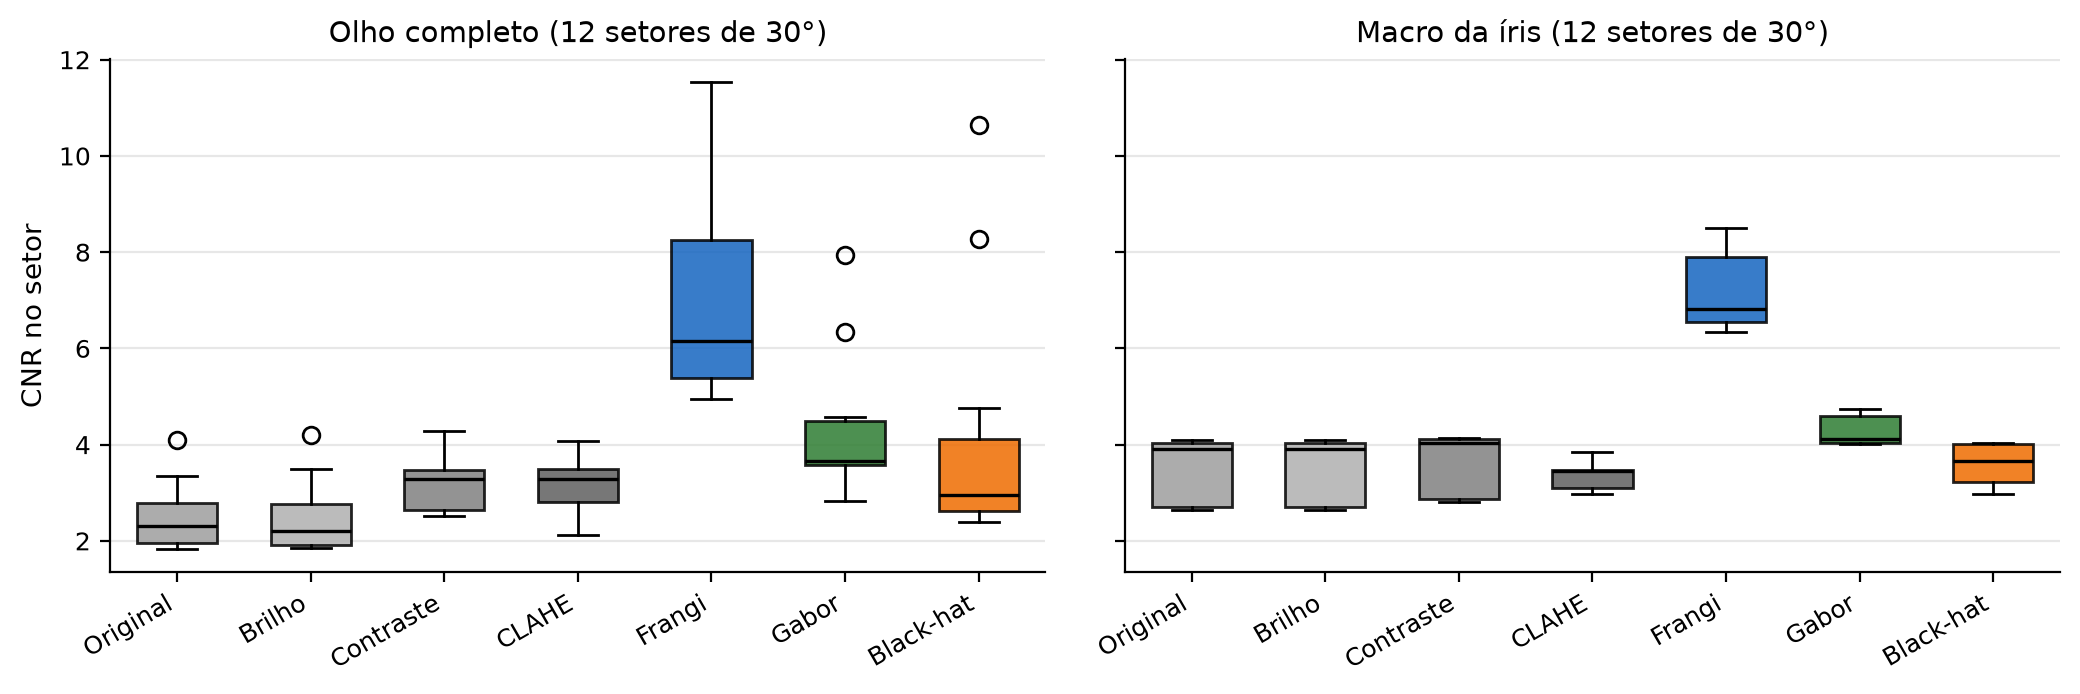
\includegraphics[width=\textwidth]{setores_cnr_boxplot.png}
  \fonte{Elaborada pelo autor (2026), a partir de fotografias de
  \citet{Novak2005} e de \citet{Reyes2014}.}
\end{figure}

\begin{figure}[htbp]
  \caption{Perfil angular da CNR para a melhor linha de base, o filtro de
  Frangi e o banco de Gabor (E1)}
  \label{fig:setores-polar}
  \centering
  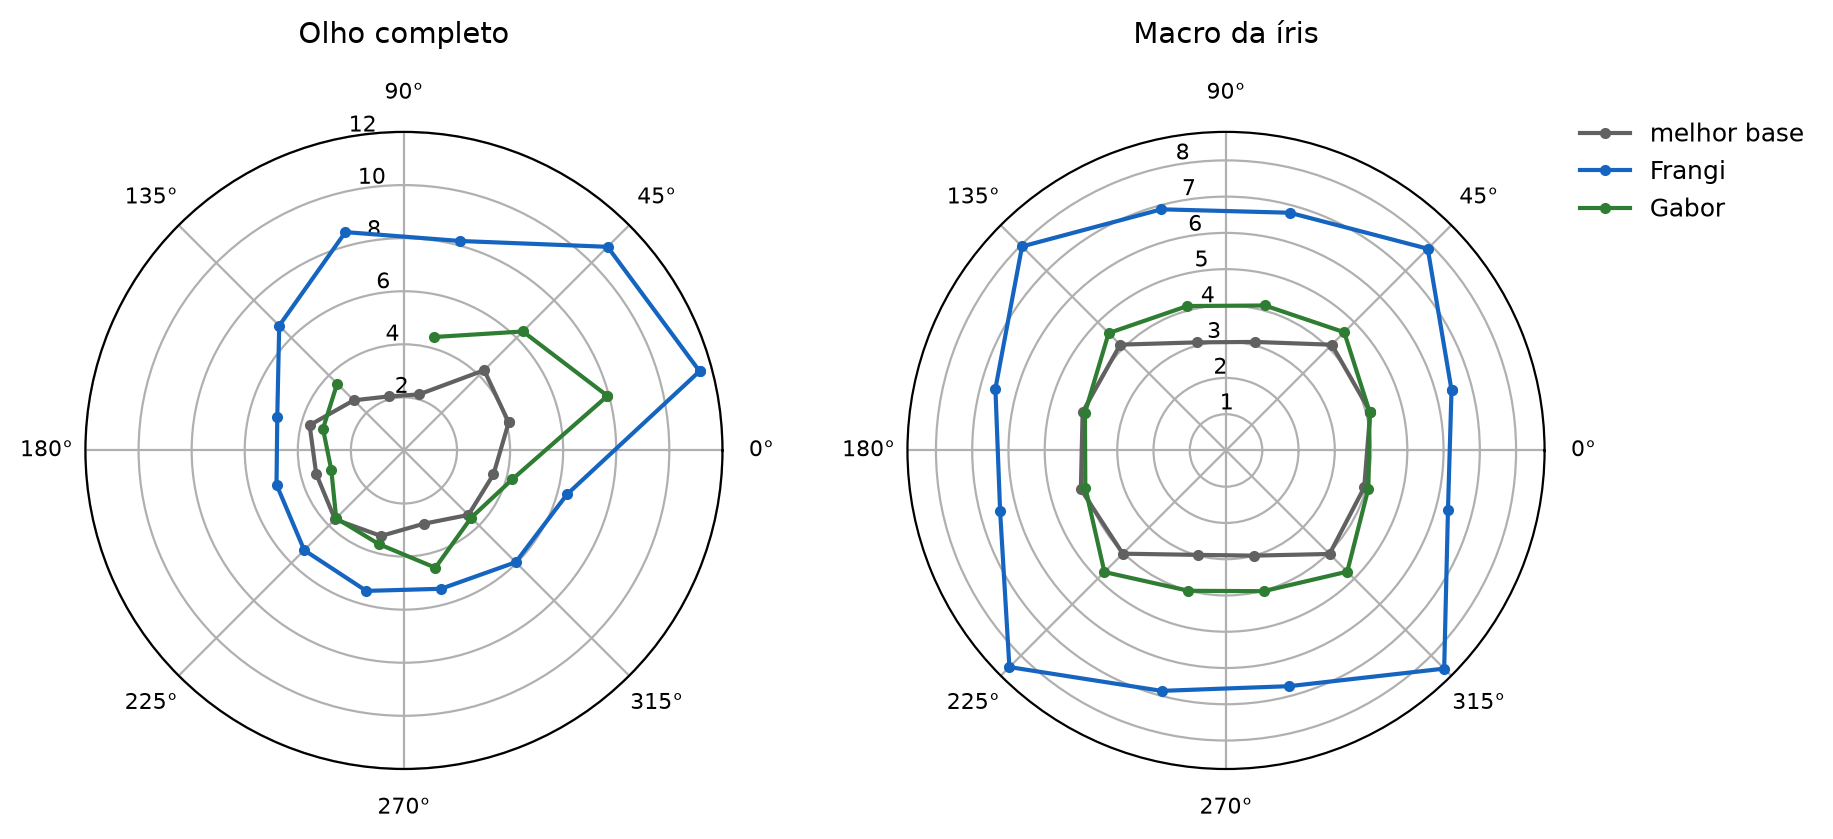
\includegraphics[width=0.92\textwidth]{setores_polar.png}
  \fonte{Elaborada pelo autor (2026), a partir de fotografias de
  \citet{Novak2005} e de \citet{Reyes2014}.}
  \nota{Ângulo medido no sentido anti-horário a partir da direita.}
\end{figure}

Os maiores valores do filtro de Frangi no olho completo ocorreram justamente
em S1 e S2 (11,53 e 10,85), onde os cílios atravessam a íris, e o realce
\bh{} também foi elevado nesses setores (10,65 e 8,26). Para verificar se a
vantagem dependia desse artefato, a análise foi repetida sem esses dois
setores (últimas linhas da Tabela~\ref{tab:setores}). O filtro de Frangi
manteve a superioridade em 10 de 10 setores, com razão mediana de 1,78
(IC~95\%: 1,45 a 2,81) e $p < 0{,}001$. O banco de Gabor passou a superar a
linha de base em 6 de 9 setores, com razão de 1,10 (IC~95\%: 0,86 a 1,60) e
$p = 0{,}082$, e o realce \bh{}, em 3 de 10. Conclui-se que a vantagem do
filtro de Frangi não é explicada pelos cílios, ao passo que a do banco de
Gabor no olho completo depende parcialmente deles.

\secao{Definição do limiar da métrica (E2)}
\label{sec:res-limiar}

A Tabela~\ref{tab:metrica-otsu} compara a CNR com o limiar de Otsu calculado
sobre o mapa inteiro, como na cadeia de análise, e restrito ao anel. A ordem
entre os realces manteve-se: o filtro de Frangi continuou com a maior CNR
(8,21 e 7,42 com o limiar no anel) e o banco de Gabor, em segundo lugar
(6,35 e 4,25). Com o limiar no anel, a melhor linha de base passou a 3,79 e
3,02, de modo que as razões do filtro de Frangi foram de 2,16 e 2,46. O filtro
de Frangi foi o método menos sensível à escolha, com variação inferior a 2\%,
o que é coerente com um mapa cujo fundo permanece próximo de zero em toda a
imagem. O realce \bh{} foi o mais sensível: sua CNR no olho completo passou de
4,38 para 5,89, e na macro ele passou a superar a melhor linha de base (3,45
contra 3,02). Esse comportamento indica que o mapa morfológico apresenta
respostas intensas fora da íris (pálpebras e cílios), que deslocam o limiar
global, e que o desempenho do realce \bh{} é o mais dependente da definição da
métrica.

\begin{table}[htbp]
  \caption{CNR com o limiar de Otsu calculado sobre o mapa inteiro e
  restrito ao anel da íris (E2)}
  \label{tab:metrica-otsu}
  \centering\footnotesize
  % Gerado por experiments/report_experiments.py (não editar à mão).
\begin{tabular}{lcccc}
\toprule
 & \multicolumn{2}{c}{Olho completo} & \multicolumn{2}{c}{Macro da íris} \\
\cmidrule(lr){2-3}\cmidrule(lr){4-5}
Método & Otsu global & Otsu no anel & Otsu global & Otsu no anel \\
\midrule
Original (verde) & 3,22 & 3,66 & 3,54 & 2,98 \\
Brilho $+40$ & 3,21 & 3,65 & 3,54 & 3,02 \\
Contraste $\times1{,}8$ & 3,49 & 3,79 & 3,62 & 2,94 \\
CLAHE & 3,26 & 3,43 & 3,34 & 2,91 \\
Frangi & 8,24 & 8,21 & 7,29 & 7,42 \\
Gabor & 5,90 & 6,35 & 4,31 & 4,25 \\
\textit{Black-hat} & 4,38 & 5,89 & 3,56 & 3,45 \\
\bottomrule
\end{tabular}

  \fonte{Elaborada pelo autor (2026).}
  \nota{Otsu global: limiar calculado sobre o mapa inteiro, padrão da cadeia
  de análise.}
\end{table}

\secao{Escalas e normalização do filtro de Frangi (E3)}
\label{sec:res-escalas}

A Tabela~\ref{tab:frangi-escalas} decompõe a resposta multiescala. A escala
$\sigma = 1$ produziu a maior resposta em 98,7\% dos pixels de estrutura do
olho completo e em 99,9\% dos da macro da íris, e a resposta média diminuiu
de 5 a 13 vezes de $\sigma = 1$ para $\sigma = 2$. O máximo das respostas
individuais coincidiu exatamente com a saída multiescala (diferença máxima
nula), o que confirma a implementação. A CNR da escala $\sigma = 1$ isolada
(8,29 e 7,33) é praticamente igual à da saída multiescala (8,24 e 7,29); o
filtro comporta-se, portanto, como um filtro de escala única. A
Figura~\ref{fig:frangi-escalas} mostra que as escalas maiores realçam fibras
mais largas (painéis c e d), mas essas respostas são encobertas no máximo.
Esse comportamento decorre da ausência de normalização das derivadas pela
escala, discutida na Seção~\ref{cap:fundamentacao}, e indica que a
normalização proposta por \citet{Lindeberg1998} constitui ajuste prioritário
para trabalhos futuros.

\begin{table}[htbp]
  \caption{Decomposição por escala da resposta do filtro de Frangi (E3)}
  \label{tab:frangi-escalas}
  \centering\footnotesize
  \setlength{\tabcolsep}{4pt}
  % Gerado por experiments/report_experiments.py (não editar à mão).
\begin{tabular}{ccccccc}
\toprule
 & \multicolumn{3}{c}{Olho completo} & \multicolumn{3}{c}{Macro da íris} \\
\cmidrule(lr){2-4}\cmidrule(lr){5-7}
$\sigma$ & Dominância (\%) & $\bar{V}_\sigma$ ($\times10^{-7}$) & CNR & Dominância (\%) & $\bar{V}_\sigma$ ($\times10^{-7}$) & CNR \\
\midrule
1 & 98,7 & 17,08 & 8,29 & 99,9 & 16,97 & 7,33 \\
2 & 1,3 & 1,29 & 8,19 & 0,1 & 3,27 & 7,05 \\
3 & 0,0 & 0,23 & 7,46 & 0,0 & 0,82 & 6,52 \\
4 & 0,0 & 0,07 & 7,02 & 0,0 & 0,26 & 6,36 \\
\midrule
Multiescala & 100,0 & -- & 8,24 & 100,0 & -- & 7,29 \\
\bottomrule
\end{tabular}

  \fonte{Elaborada pelo autor (2026).}
  \nota{Dominância: fração dos pixels de estrutura em que a escala produz a
  maior resposta; $\bar{V}_\sigma$: resposta bruta média no anel; CNR: escala
  isolada, com a mesma normalização de saída.}
\end{table}

\begin{figure}[htbp]
  \caption{Respostas do filtro de Frangi por escala, saída multiescala e
  escala dominante na macro da íris (E3)}
  \label{fig:frangi-escalas}
  \centering
  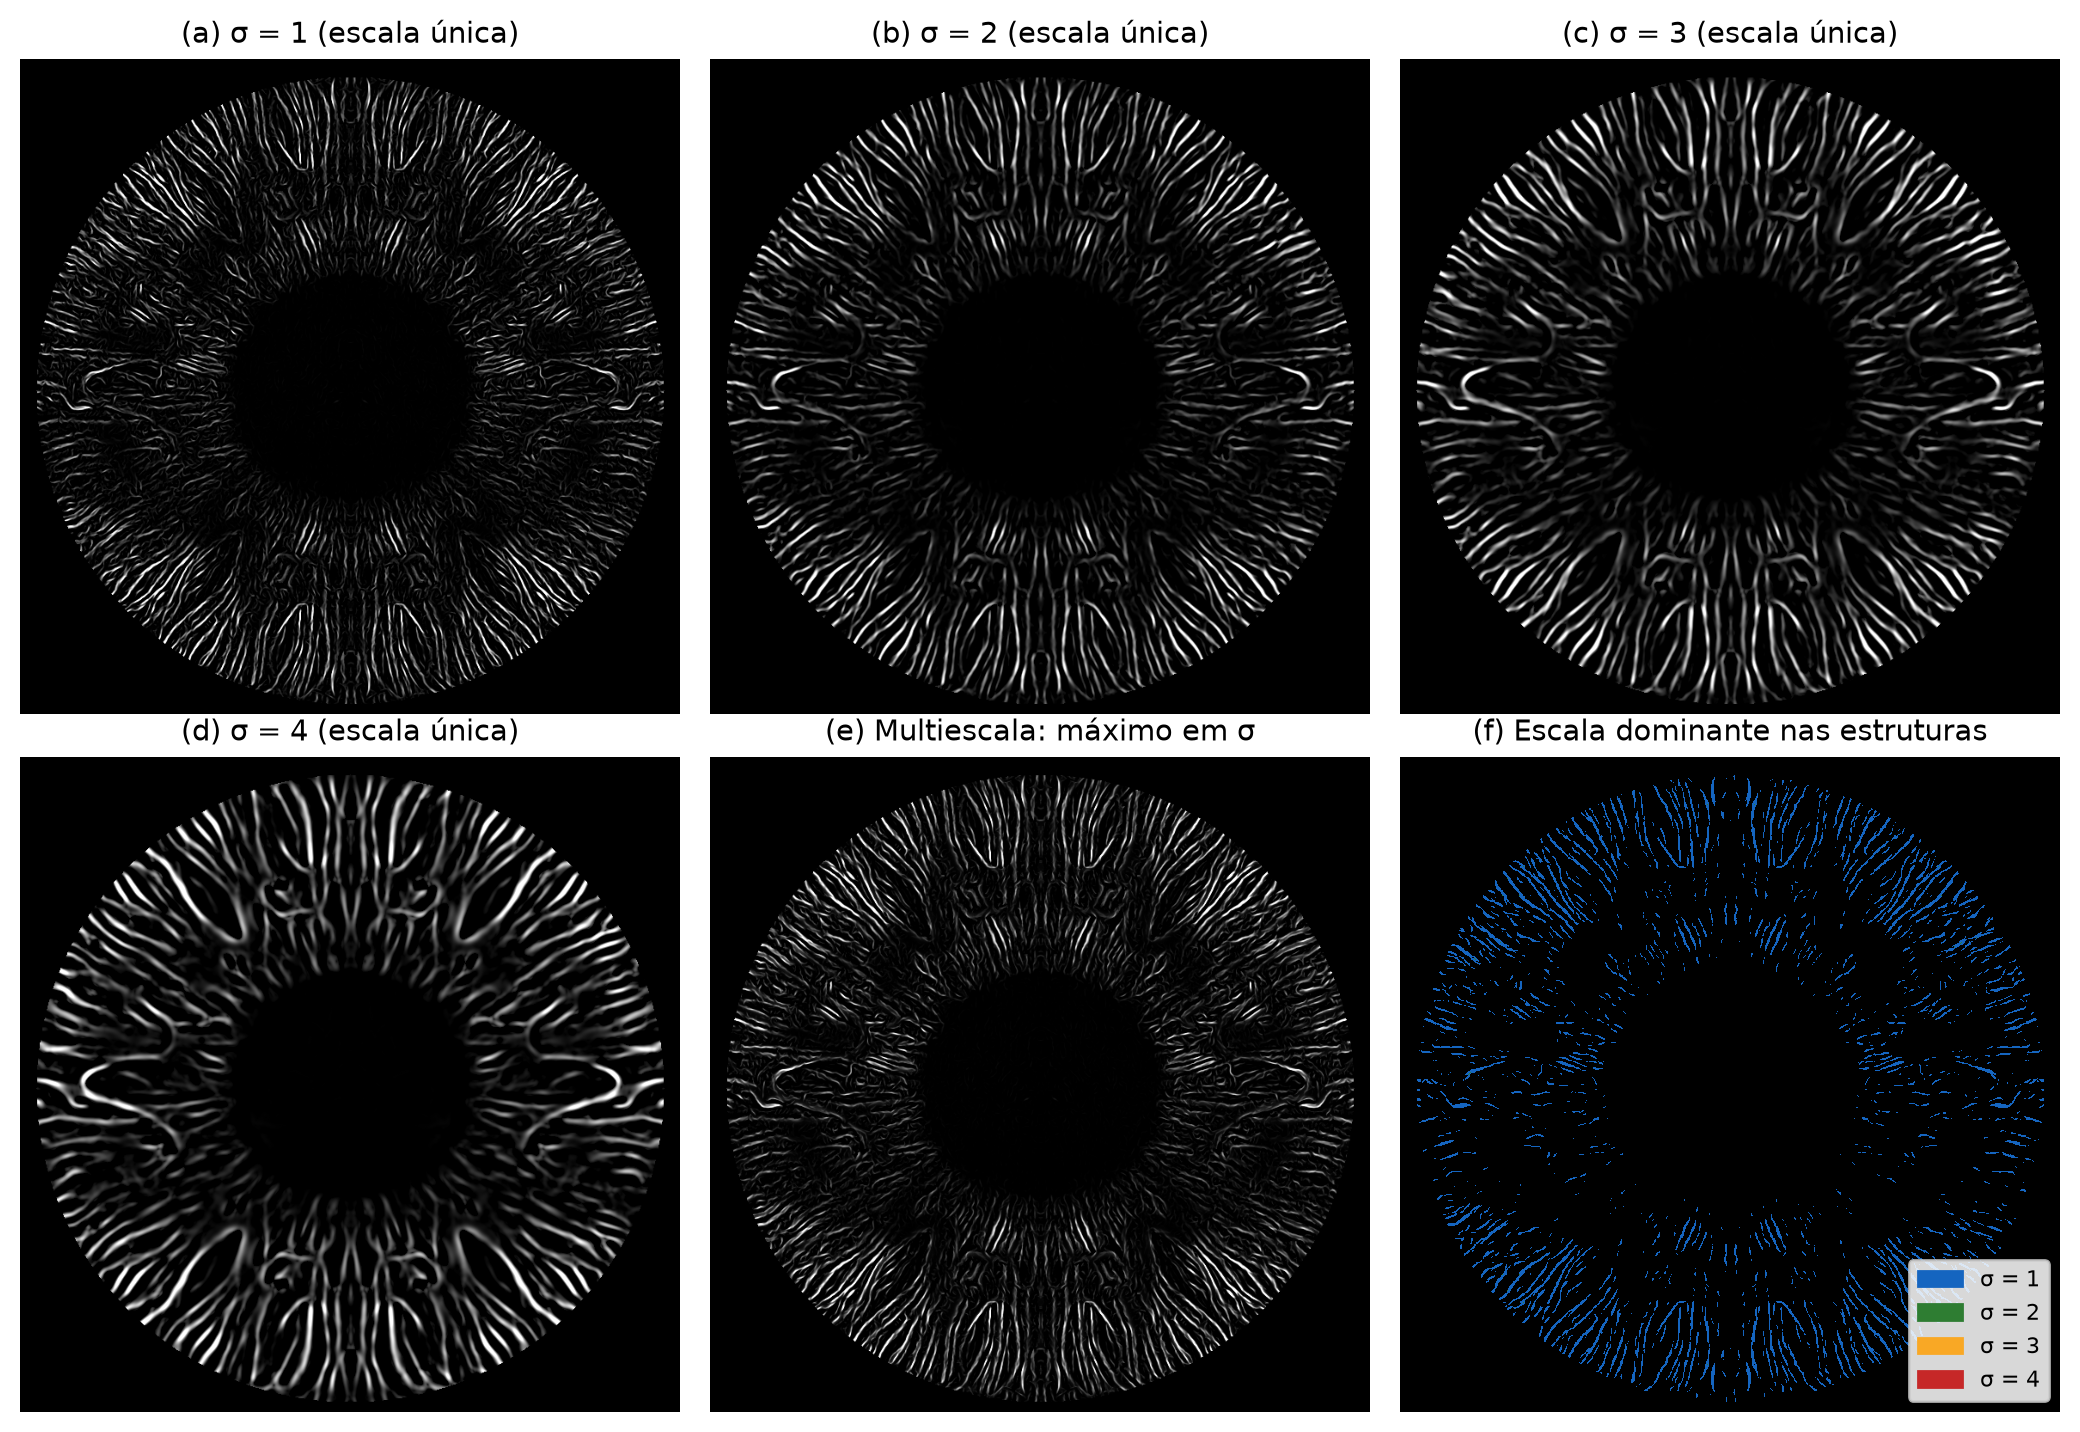
\includegraphics[width=0.97\textwidth]{frangi_escalas_closeup.png}
  \fonte{Elaborada pelo autor (2026), a partir de fotografia de
  \citet{Reyes2014}.}
  \nota{Cada painel possui normalização própria.}
\end{figure}

A Tabela~\ref{tab:frangi-normalizacao} mostra o efeito da normalização de
saída sobre a CNR do mesmo mapa de Frangi. Sem a correção gama, a CNR sobe
para 12,01 e 9,99; com normalização mínimo--máximo, para 24,39 e 10,70. Todas
essas normalizações são crescentes e preservam a ordenação dos pixels, mas,
conforme observado após a Proposição~1, alteram a CNR. O valor muito elevado
obtido com a normalização mínimo--máximo no olho completo é o efeito esperado
quando poucas respostas muito intensas, como as dos cílios, comprimem as
demais próximo de zero e reduzem $\sigma_{\text{bg}}$. Duas consequências
decorrem desse resultado. Primeiro, a normalização adotada é a mais
conservadora das três, de modo que a comparação da
Seção~\ref{sec:res-principal} não favorece o filtro de Frangi. Segundo,
valores absolutos de CNR só são comparáveis sob a mesma normalização, o que
reforça a necessidade de uma medida invariante, como a AUC do fantoma
(Seção~\ref{sec:res-fantoma}).

\begin{table}[htbp]
  \caption{Efeito da normalização de saída sobre a CNR do mapa de Frangi
  (E3)}
  \label{tab:frangi-normalizacao}
  \centering\footnotesize
  % Gerado por experiments/report_experiments.py (não editar à mão).
\begin{tabular}{lcc}
\toprule
Normalização do mapa de Frangi & CNR (Olho completo) & CNR (Macro da íris) \\
\midrule
Percentis 2 e 99 com gama 0,7 (padrão) & 8,24 & 7,29 \\
Percentis 2 e 99, sem gama & 12,01 & 9,99 \\
Mínimo--máximo & 24,39 & 10,70 \\
\bottomrule
\end{tabular}

  \fonte{Elaborada pelo autor (2026).}
  \nota{As três transformações são crescentes; a primeira é a adotada na
  cadeia de análise.}
\end{table}

\secao{Sensibilidade a parâmetros (E4)}
\label{sec:res-sensibilidade}

A Tabela~\ref{tab:sensibilidade} apresenta a CNR obtida quando cada parâmetro
é variado isoladamente. No filtro de Frangi, a CNR variou entre 6,95 e 9,15 no
olho completo e entre 6,29 e 7,85 na macro da íris. O menor valor ocorreu com
$c = 0{,}05$: com $c$ pequeno, o termo de estruturalidade satura e respostas
fracas do fundo passam a valer tanto quanto as fibras. Valores menores de
$\beta$ aumentaram a CNR ($\beta = 0{,}25$: 9,15 e 7,85), por tornarem o
filtro mais seletivo a linhas. A remoção da escala $\sigma = 1$ reduziu a CNR
(8,15 e 6,99), e o acréscimo de $\sigma = 5$ e $\sigma = 6$ não teve efeito,
o que é coerente com a dominância da escala mais fina.

\begin{table}[htbp]
  \caption{Sensibilidade da CNR aos parâmetros de cada realce (E4)}
  \label{tab:sensibilidade}
  \centering\footnotesize
  % Gerado por experiments/report_experiments.py (não editar à mão).
\begin{tabular}{lllcc}
\toprule
Algoritmo & Parâmetro & Valor & CNR (Olho completo) & CNR (Macro da íris) \\
\midrule
Frangi & $\beta$ & 0,25 & 9,15 & 7,85 \\
 &  & \textbf{0,50}$^\ast$ & \textbf{8,24} & \textbf{7,29} \\
 &  & 0,75 & 7,94 & 7,10 \\
 &  & 1,00 & 7,81 & 7,01 \\
\cmidrule(lr){2-5}
 & $c$ & 0,05 & 6,95 & 6,29 \\
 &  & 0,25 & 8,14 & 7,23 \\
 &  & 1,00 & 8,24 & 7,29 \\
 &  & \textbf{15,00}$^\ast$ & \textbf{8,24} & \textbf{7,29} \\
\cmidrule(lr){2-5}
 & $\{\sigma\}$ & \{1\} & 8,29 & 7,33 \\
 &  & \{1, 2\} & 8,23 & 7,27 \\
 &  & \textbf{\{1, 2, 3, 4\}}$^\ast$ & \textbf{8,24} & \textbf{7,29} \\
 &  & \{2, 3, 4\} & 8,15 & 6,99 \\
 &  & \{1, 2, 3, 4, 5, 6\} & 8,24 & 7,30 \\
\midrule
Gabor & $\lambda$ & 6 & 7,02 & 4,75 \\
 &  & 8 & 6,41 & 4,50 \\
 &  & \textbf{10}$^\ast$ & \textbf{5,90} & \textbf{4,31} \\
 &  & 14 & 5,31 & 4,17 \\
\cmidrule(lr){2-5}
 & $\sigma$ & 2 & 5,31 & 4,21 \\
 &  & 3 & 5,68 & 4,25 \\
 &  & \textbf{4}$^\ast$ & \textbf{5,90} & \textbf{4,31} \\
 &  & 6 & 6,41 & 4,33 \\
\cmidrule(lr){2-5}
 & $n_\theta$ & 4 & 5,44 & 4,39 \\
 &  & \textbf{8}$^\ast$ & \textbf{5,90} & \textbf{4,31} \\
 &  & 12 & 5,92 & 4,27 \\
\midrule
Morfologia & escalas & \{5\} & 7,63 & 4,50 \\
 &  & \{11\} & 5,06 & 3,79 \\
 &  & \{21\} & 3,89 & 3,47 \\
 &  & \textbf{\{5, 11, 21\}}$^\ast$ & \textbf{4,38} & \textbf{3,56} \\
 &  & \{5, 11, 21, 31\} & 3,95 & 3,43 \\
\bottomrule
\end{tabular}

  \fonte{Elaborada pelo autor (2026).}
  \nota{Cada parâmetro é variado isoladamente; o asterisco e o negrito
  indicam a configuração padrão. Na varredura de $\sigma$ do filtro de Gabor,
  o núcleo cresce para cobrir a envoltória.}
\end{table}

No banco de Gabor, comprimentos de onda menores aumentaram a CNR
($\lambda = 6$: 7,02 e 4,75, contra 5,90 e 4,31 com $\lambda = 10$), o que
sugere que as fibras visíveis nessas imagens são mais finas que as
sintonizadas pela configuração padrão. O aumento de $\sigma$ elevou a CNR no
olho completo (6,41 com $\sigma = 6$), mas quase não a alterou na macro da
íris,
e a passagem de 8 para 12 orientações teve efeito desprezível. Na morfologia,
o elemento de 5 pixels isolado produziu a maior CNR (7,63 e 4,50), e os
elementos maiores reduziram-na; a soma padrão de três escalas (4,38 e 3,56)
ficou abaixo do elemento menor, pois os elementos grandes acrescentam
respostas de baixa frequência, como sombras e regiões extensas, que diluem as
estruturas finas.

Em todas as configurações testadas, o filtro de Frangi e o banco de Gabor
permaneceram acima da melhor linha de base das duas imagens (3,49 e 3,62), ao
passo que o realce \bh{} ficou abaixo dela na macro da íris em três das cinco
configurações. As configurações de maior CNR não foram adotadas como padrão,
pois foram observadas nas mesmas duas imagens empregadas na avaliação, e sua
adoção tornaria a comparação otimista. Essa escolha deve ser feita no
conjunto rotulado, com dados de ajuste separados dos dados de teste.

\secao{Escolha do canal de cor (E10)}
\label{sec:res-canal}

A Tabela~\ref{tab:canais} compara os canais de entrada. O canal azul produziu
a maior CNR nas seis comparações: no próprio canal (3,78 e 3,81), após o
filtro de Frangi (8,61 e 7,57) e após o banco de Gabor (6,14 e 4,62). O canal
verde, padrão da cadeia de análise, ficou em segundo lugar após o filtro de
Frangi (8,24 e 7,29), e o vermelho apresentou o pior resultado do filtro de
Frangi no olho completo (7,33). As diferenças entre os canais azul e verde são
pequenas (entre 3,8\% e 4,5\% no filtro de Frangi) e foram observadas em duas
íris de cor clara. Uma hipótese, não testada neste trabalho, é a de que,
nessas íris, o contraste do estroma dependa mais do espalhamento da luz, mais
intenso em comprimentos de onda curtos. O canal verde foi mantido por
coerência com a literatura de retina, mas a escolha deve ser reavaliada no
conjunto rotulado, com íris de diferentes pigmentações.

\begin{table}[htbp]
  \caption{CNR no anel por canal de entrada (E10)}
  \label{tab:canais}
  \centering\footnotesize
  % Gerado por experiments/report_experiments.py (não editar à mão).
\begin{tabular}{lcccccc}
\toprule
 & \multicolumn{3}{c}{Olho completo} & \multicolumn{3}{c}{Macro da íris} \\
\cmidrule(lr){2-4}\cmidrule(lr){5-7}
Canal & Canal & Frangi & Gabor & Canal & Frangi & Gabor \\
\midrule
Vermelho (R) & 3,25 & 7,33 & 5,76 & 3,63 & 7,21 & 4,24 \\
Verde (G)$^\ast$ & 3,22 & 8,24 & 5,90 & 3,54 & 7,29 & 4,31 \\
Azul (B) & 3,78 & 8,61 & 6,14 & 3,81 & 7,57 & 4,62 \\
Luminância (Y) & 3,30 & 8,10 & 5,91 & 3,55 & 7,28 & 4,30 \\
\bottomrule
\end{tabular}

  \fonte{Elaborada pelo autor (2026).}
  \nota{O asterisco indica o canal padrão da cadeia de análise.}
\end{table}

\secao{Robustez a perturbações (E5)}
\label{sec:res-robustez}

A Tabela~\ref{tab:robustez} mostra a concordância entre os mapas obtidos com
e sem cada perturbação. Sob perturbações fotométricas (brilho, contraste e
correção gama), todos os métodos mantiveram correlação de pelo menos 0,99 e
coeficiente de Dice de pelo menos 0,91, resultado esperado porque a CLAHE
renormaliza o contraste local antes dos realces. As perturbações que alteram a
estrutura fina distinguiram os métodos. O filtro de Frangi foi o mais
afetado: correlação de 0,90 e Dice de 0,75 com ruído, de 0,81 e 0,65 com
desfoque e de 0,92 e 0,78 com compressão JPEG. O banco de Gabor foi o mais
estável, com Dice médio de pelo menos 0,86 em todas as condições, e o realce
\bh{} ocupou posição intermediária. A Figura~\ref{fig:robustez} ilustra o
efeito sobre o filtro de Frangi: a alteração fotométrica quase não modifica o
mapa, o ruído cria cristas espúrias e o desfoque funde as fibras finas.

\begin{table}[htbp]
  \caption{Concordância entre os mapas sem e com perturbação (E5)}
  \label{tab:robustez}
  \centering\footnotesize
  \setlength{\tabcolsep}{4.5pt}
  % Gerado por experiments/report_experiments.py (não editar à mão).
\begin{tabular}{lcccccccc}
\toprule
Perturbação & \multicolumn{2}{c}{CLAHE} & \multicolumn{2}{c}{Frangi} & \multicolumn{2}{c}{Gabor} & \multicolumn{2}{c}{\textit{Black-hat}} \\
\cmidrule(lr){2-3}\cmidrule(lr){4-5}\cmidrule(lr){6-7}\cmidrule(lr){8-9}
 & $r$ & Dice & $r$ & Dice & $r$ & Dice & $r$ & Dice \\
\midrule
Brilho $-30$ & 0,99 & 0,96 & 1,00 & 0,98 & 1,00 & 0,97 & 1,00 & 0,96 \\
Brilho $+30$ & 1,00 & 0,96 & 1,00 & 0,99 & 1,00 & 0,99 & 1,00 & 0,99 \\
Contraste $\times0{,}7$ & 0,99 & 0,97 & 1,00 & 0,94 & 1,00 & 0,94 & 1,00 & 0,91 \\
Contraste $\times1{,}3$ & 0,99 & 0,95 & 0,99 & 0,97 & 0,99 & 0,97 & 0,99 & 0,98 \\
Gama $0{,}7$ & 1,00 & 0,97 & 1,00 & 0,95 & 1,00 & 0,96 & 0,99 & 0,95 \\
Gama $1{,}5$ & 0,99 & 0,92 & 0,99 & 0,93 & 0,99 & 0,94 & 0,99 & 0,93 \\
Ruído gaussiano ($\sigma=8$) & 0,96 & 0,92 & 0,90 & 0,75 & 0,99 & 0,94 & 0,92 & 0,77 \\
Desfoque gaussiano ($\sigma=1{,}5$) & 0,97 & 0,94 & 0,81 & 0,65 & 0,98 & 0,86 & 0,90 & 0,77 \\
Compressão JPEG ($q=30$) & 0,99 & 0,95 & 0,92 & 0,78 & 0,99 & 0,95 & 0,97 & 0,88 \\
\midrule
Média & \textbf{0,99} & \textbf{0,95} & \textbf{0,96} & \textbf{0,88} & \textbf{0,99} & \textbf{0,95} & \textbf{0,97} & \textbf{0,90} \\
\bottomrule
\end{tabular}

  \fonte{Elaborada pelo autor (2026).}
  \nota{Média das duas imagens. $r$: correlação de Pearson no anel; Dice:
  sobreposição das máscaras de estrutura.}
\end{table}

\begin{figure}[htbp]
  \caption{Trecho do mapa de Frangi sem perturbação e sob correção gama, ruído
  gaussiano e desfoque (E5)}
  \label{fig:robustez}
  \centering
  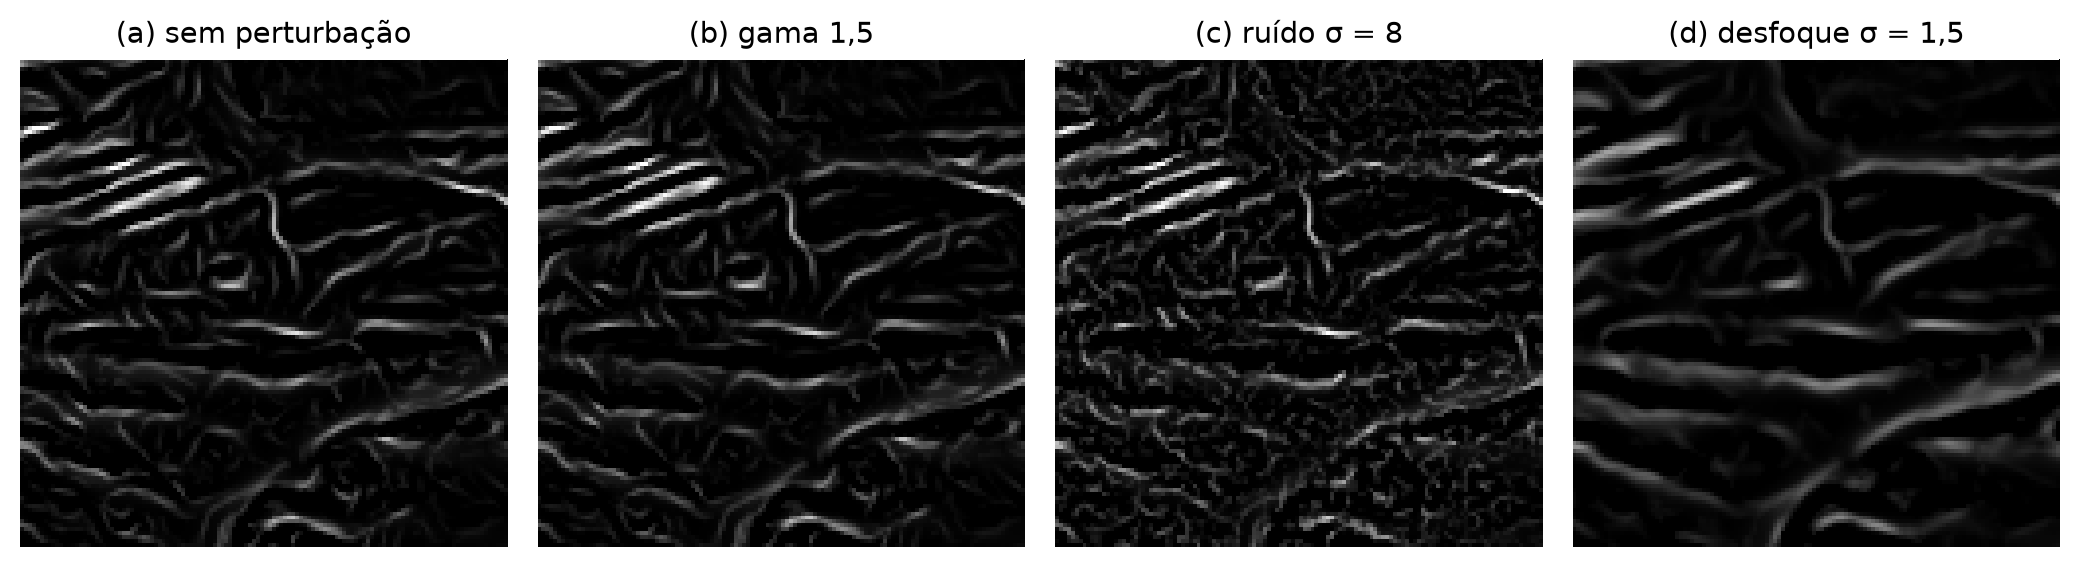
\includegraphics[width=\textwidth]{robustez_frangi_exemplo.png}
  \fonte{Elaborada pelo autor (2026), a partir de fotografia de
  \citet{Reyes2014}.}
\end{figure}

A razão entre a CNR com e sem perturbação ficou entre 0,78 e 1,10 para o
filtro de Frangi, entre 0,96 e 1,13 para o banco de Gabor, entre 0,83 e 1,27
para o realce \bh{} e entre 0,93 e 1,11 para a CLAHE. O máximo do filtro de
Frangi ocorreu com desfoque no olho completo, a mesma perturbação em que o
Dice médio se reduziu a 0,65: a CNR permaneceu elevada enquanto o conjunto de
estruturas detectadas se alterou. A CNR mede quanto o mapa separa duas
classes, e não se as estruturas são as mesmas; por esse motivo, a robustez
deve ser avaliada com medidas de concordância, como o coeficiente de Dice e a
correlação. A sensibilidade do filtro de Frangi ao ruído e ao desfoque é
coerente com a dominância da escala $\sigma = 1$, a mais afetada por esses
dois fatores.

\secao{Fantoma com verdade de referência (E6)}
\label{sec:res-fantoma}

A Figura~\ref{fig:fantoma} mostra um fantoma com ruído $\sigma_n = 12$ e os
mapas correspondentes, e a Tabela~\ref{tab:fantoma} resume as medidas nesse
nível de ruído. O fantoma confirma a Proposição~1: o original e o brilho
$+40$ apresentaram a mesma AUC até a sexta casa decimal em todos os níveis de
ruído (0,685 com $\sigma_n = 12$), e o contraste $\times 1{,}8$ diferiu em
menos de 0,001, por efeito da saturação. Na figura, observa-se que o filtro
de Frangi responde também ao ruído fino, que o banco de Gabor preserva a
continuidade das curvas e que o realce \bh{} responde às manchas da textura
de fundo.

\begin{figure}[htbp]
  \caption{Fantoma sintético com ruído $\sigma_n = 12$, verdade de referência
  e mapas de realce (E6)}
  \label{fig:fantoma}
  \centering
  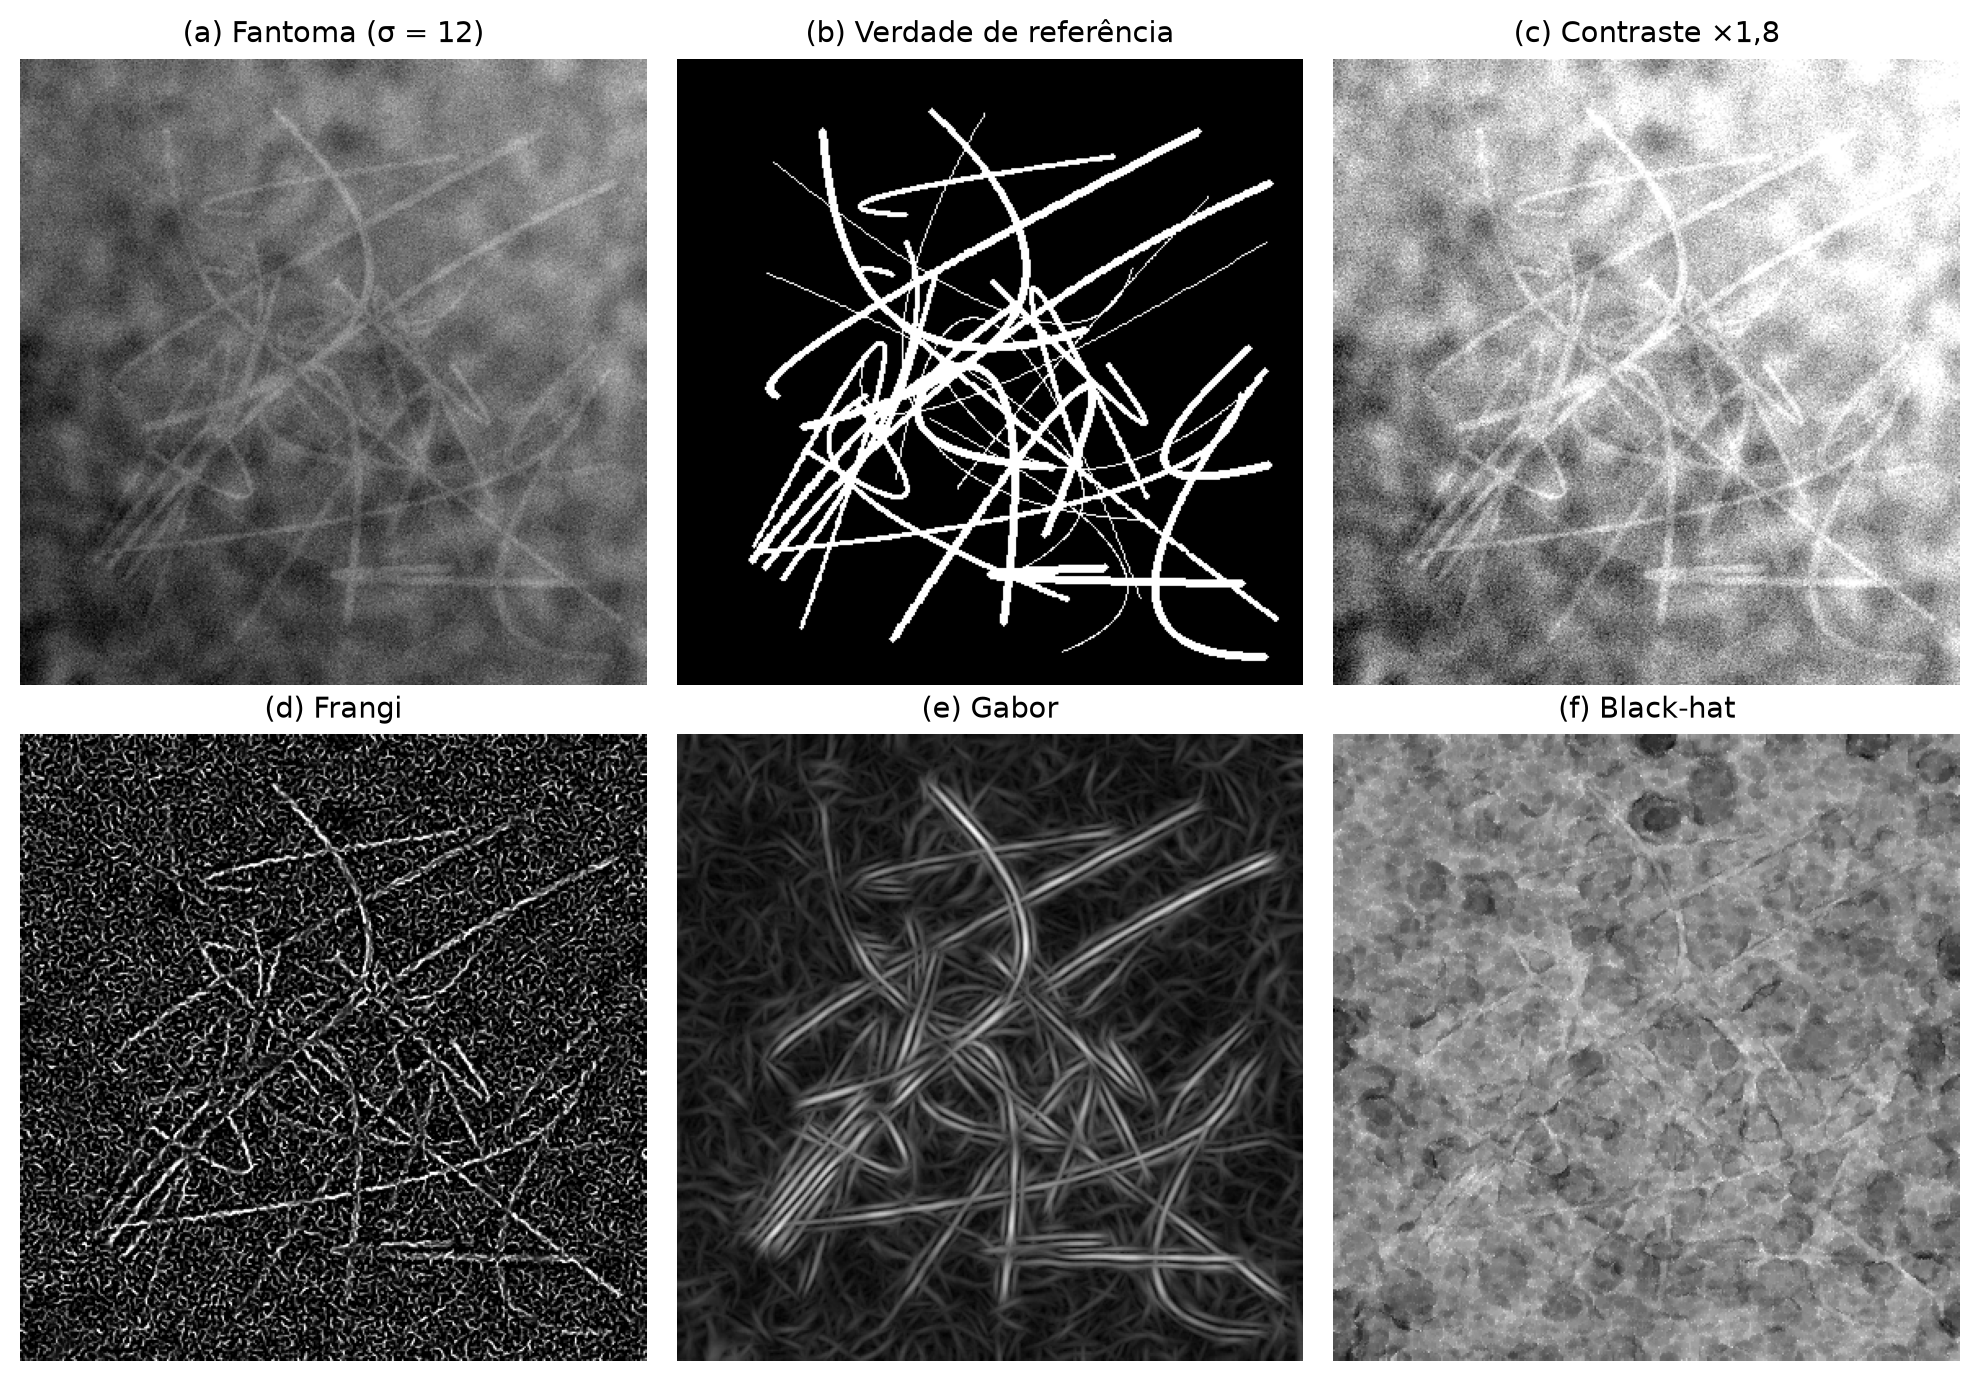
\includegraphics[width=0.95\textwidth]{fantoma_exemplo.png}
  \fonte{Elaborada pelo autor (2026).}
\end{figure}

\begin{table}[htbp]
  \caption{Medidas no fantoma com ruído $\sigma_n = 12$ (E6)}
  \label{tab:fantoma}
  \centering\footnotesize
  % Gerado por experiments/report_experiments.py (não editar à mão).
\begin{tabular}{lccc}
\toprule
Método & AUC (média $\pm$ dp) & CNR com verdade & CNR por Otsu \\
\midrule
Original (verde) & 0,685 $\pm$ 0,029 & 0,65 & 2,78 \\
Brilho $+40$ & 0,685 $\pm$ 0,029 & 0,65 & 2,78 \\
Contraste $\times1{,}8$ & 0,684 $\pm$ 0,028 & 0,64 & 2,77 \\
CLAHE & 0,751 $\pm$ 0,020 & 0,95 & 2,87 \\
\midrule
Frangi & 0,757 $\pm$ 0,011 & 1,06 & 5,44 \\
Gabor & \textbf{0,879} $\pm$ \textbf{0,013} & 2,44 & 4,68 \\
\textit{Black-hat} & 0,628 $\pm$ 0,017 & 0,48 & 2,58 \\
\bottomrule
\end{tabular}

  \fonte{Elaborada pelo autor (2026).}
  \nota{Média de 10 sementes. AUC por pixel com desvio-padrão (dp) entre
  sementes; CNR com verdade: estrutura e fundo definidos pela máscara
  verdadeira; CNR por Otsu: medida empregada nas imagens reais.}
\end{table}

A Figura~\ref{fig:auc-ruido} apresenta a AUC em função do ruído. Com ruído
baixo ($\sigma_n = 4$), o filtro de Frangi obteve a maior AUC (0,919),
seguido do banco de Gabor (0,902), do realce \bh{} (0,869), da CLAHE (0,805)
e do original (0,701). Com o aumento do ruído, o filtro de Frangi degradou
rapidamente (0,827, 0,757, 0,711 e 0,657), igualando-se à CLAHE a partir de
$\sigma_n = 12$ e aproximando-se do original com $\sigma_n = 24$. O banco de
Gabor degradou lentamente (0,894, 0,879, 0,859 e 0,812) e foi o melhor método
a partir de $\sigma_n = 8$. O realce \bh{} apresentou desempenho inferior ao
acaso com $\sigma_n = 24$ (AUC de 0,482): por somar as duas polaridades, ele
responde também às manchas escuras da textura de fundo, visíveis na
Figura~\ref{fig:fantoma}. As curvas ROC da Figura~\ref{fig:roc} confirmam
esse quadro com $\sigma_n = 12$.

\begin{figure}[htbp]
  \caption{AUC por pixel em função do desvio-padrão do ruído no fantoma
  (E6)}
  \label{fig:auc-ruido}
  \centering
  \begin{tikzpicture}
    \begin{axis}[
      width=0.62\textwidth, height=6.4cm,
      xlabel={desvio-padrão do ruído $\sigma_n$},
      ylabel={AUC (média de 10 fantomas)},
      xtick={4,8,12,16,24}, ymin=0.45, ymax=0.95,
      ymajorgrids, grid style={gray!25},
      legend style={at={(1.03,0.5)}, anchor=west, font=\small, draw=none},
      legend cell align=left,
      /pgf/number format/fixed, /pgf/number format/precision=2]
      \addplot[gray, dashed, mark=o, mark options={solid}]
        table[x=sigma, y=Original] {dados/auc_ruido.dat};
      \addplot[black!55, densely dashed, mark=square, mark options={solid}]
        table[x=sigma, y=Contraste] {dados/auc_ruido.dat};
      \addplot[black, dashdotted, mark=triangle, mark options={solid}]
        table[x=sigma, y=CLAHE] {dados/auc_ruido.dat};
      \addplot[blue!75!black, thick, mark=*,
               error bars/.cd, y dir=both, y explicit]
        table[x=sigma, y=Frangi, y error=Frangi_sd] {dados/auc_ruido.dat};
      \addplot[green!45!black, thick, mark=diamond*,
               error bars/.cd, y dir=both, y explicit]
        table[x=sigma, y=Gabor, y error=Gabor_sd] {dados/auc_ruido.dat};
      \addplot[orange!85!black, thick, mark=triangle*,
               error bars/.cd, y dir=both, y explicit]
        table[x=sigma, y=Blackhat, y error=Blackhat_sd] {dados/auc_ruido.dat};
      \addplot[gray, dotted, domain=4:24, samples=2] {0.5};
      \legend{Original ($=$ brilho $+40$), Contraste $\times1{,}8$, CLAHE,
              Frangi, Gabor, \emph{Black-hat}, acaso}
    \end{axis}
  \end{tikzpicture}
  \fonte{Elaborada pelo autor (2026).}
  \nota{Barras de um desvio-padrão entre sementes para os realces.}
\end{figure}

\begin{figure}[htbp]
  \caption{Curvas ROC agregadas no fantoma com $\sigma_n = 12$ (E6)}
  \label{fig:roc}
  \centering
  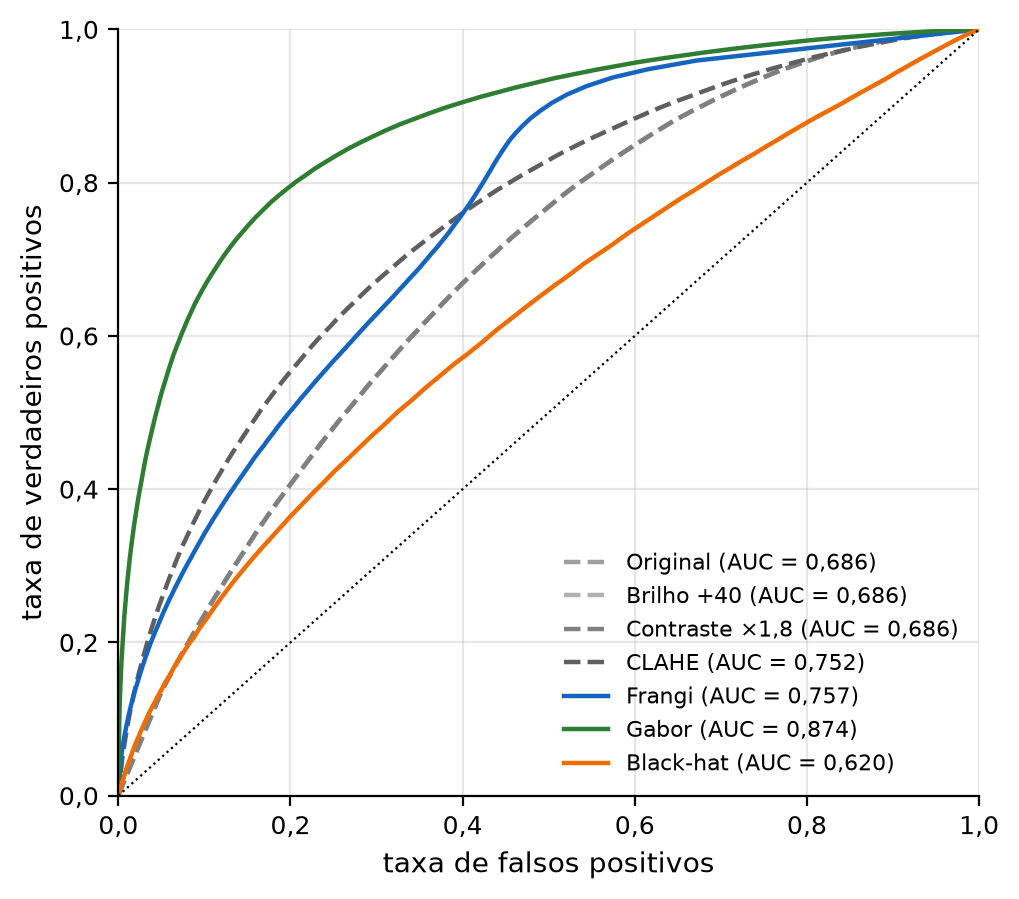
\includegraphics[width=0.58\textwidth]{fantoma_roc.png}
  \fonte{Elaborada pelo autor (2026).}
  \nota{Curvas obtidas com a reunião dos pixels das 10 sementes; a AUC da
  legenda difere ligeiramente da média por semente da
  Tabela~\ref{tab:fantoma}.}
\end{figure}

A comparação entre a CNR por Otsu e as medidas com verdade de referência
constitui o resultado mais importante do fantoma para a interpretação das
imagens reais. Nas 35 combinações de ruído e método, a CNR por Otsu
apresentou correlação de Spearman de 0,76 com a AUC e de 0,73 com a CNR com
verdade (ambas com $p < 0{,}001$): a métrica sem verdade de referência ordena
os métodos de forma semelhante, mas não idêntica, à métrica com verdade. A
discordância mais evidente envolve o filtro de Frangi. Com $\sigma_n = 12$,
ele obteve a maior CNR por Otsu (5,44) e uma AUC (0,757) muito inferior à do
banco de Gabor (0,879); entre $\sigma_n = 12$ e $\sigma_n = 24$, sua CNR por
Otsu permaneceu em 5,44, enquanto a AUC se reduziu de 0,757 para 0,657. Um
mapa esparso separa bem duas classes mesmo quando parte da estrutura
detectada é ruído, e a CNR por Otsu não distingue essas duas situações. A
vantagem do filtro de Frangi nas imagens reais deve, portanto, ser
interpretada com essa ressalva: ela é compatível com o regime de ruído baixo,
no qual o filtro de Frangi também é o melhor segundo a AUC, mas a CNR por
Otsu, isoladamente, não permite afirmar em qual regime as imagens se
encontram.

\secao{Custo computacional (E7)}
\label{sec:res-custo}

A Tabela~\ref{tab:tempo} apresenta o tempo de cada etapa em uma imagem de
$768 \times 513$ pixels. O filtro de Frangi foi a etapa mais custosa, com
mediana de 659~ms, cerca de 12 vezes a do banco de Gabor (56~ms) e 46 vezes a
do realce \bh{} (14~ms); brilho, contraste e CLAHE demandaram menos de
0,5~ms. A detecção da pupila e do limbo demandou 24,5~ms, e a validação
geométrica, alguns microssegundos. Mesmo o filtro de Frangi é viável para
processamento em lote, pois mil imagens demandariam cerca de 11 minutos em um
único núcleo. Os valores absolutos dependem da carga da máquina: em outras
execuções do mesmo \emph{script} ao longo deste trabalho, a mediana do filtro
de Frangi variou entre aproximadamente 0,65 e 0,9~s e atingiu 1,4~s com outro
processo intensivo em paralelo. A ordem relativa entre os métodos, contudo,
foi a mesma em todas as execuções.

\begin{table}[htbp]
  \caption{Tempo de execução por etapa (E7)}
  \label{tab:tempo}
  \centering\footnotesize
  % Gerado por experiments/report_experiments.py (não editar à mão).
\begin{tabular}{lccc}
\toprule
Etapa & Mediana (ms) & Mínimo (ms) & Máximo (ms) \\
\midrule
Brilho $+40$ & 0,15 & 0,15 & 0,18 \\
Contraste $\times1{,}8$ & 0,15 & 0,15 & 0,16 \\
CLAHE & 0,46 & 0,40 & 0,60 \\
Frangi & 659,1 & 617,1 & 766,1 \\
Gabor & 55,9 & 49,2 & 62,7 \\
\textit{Black-hat} & 14,3 & 13,2 & 14,8 \\
\midrule
Detecção pupila/íris & 24,5 & 22,6 & 26,5 \\
Validação geométrica & 0,003 & 0,002 & 0,009 \\
\bottomrule
\end{tabular}

  \fonte{Elaborada pelo autor (2026).}
  \nota{Valores em milissegundos: mediana, mínimo e máximo de sete execuções
  após uma de aquecimento, em processador Intel Core i7 de 12.ª geração.}
\end{table}

\secao{Normalização polar e perfil radial (E8)}
\label{sec:res-polar}

A Figura~\ref{fig:rubber} mostra o anel do olho completo desdobrado em
coordenadas polares, para o canal verde com CLAHE e para o mapa de Frangi,
com o raio crescendo da borda pupilar, na parte superior, para o limbo, na
parte inferior. A faixa de cílios aparece entre aproximadamente $15^\circ$ e
$65^\circ$ e domina o mapa de Frangi nessa região, ao passo que o reflexo
claro entre $0^\circ$ e $40^\circ$ aparece no canal verde. Fora dessas
regiões, o mapa evidencia as fibras radiais como linhas aproximadamente
verticais, isto é, alinhadas com a direção radial.

\begin{figure}[htbp]
  \caption{Anel do olho completo desdobrado pela normalização \emph{rubber
  sheet}: canal verde com CLAHE e mapa de Frangi (E8)}
  \label{fig:rubber}
  \centering
  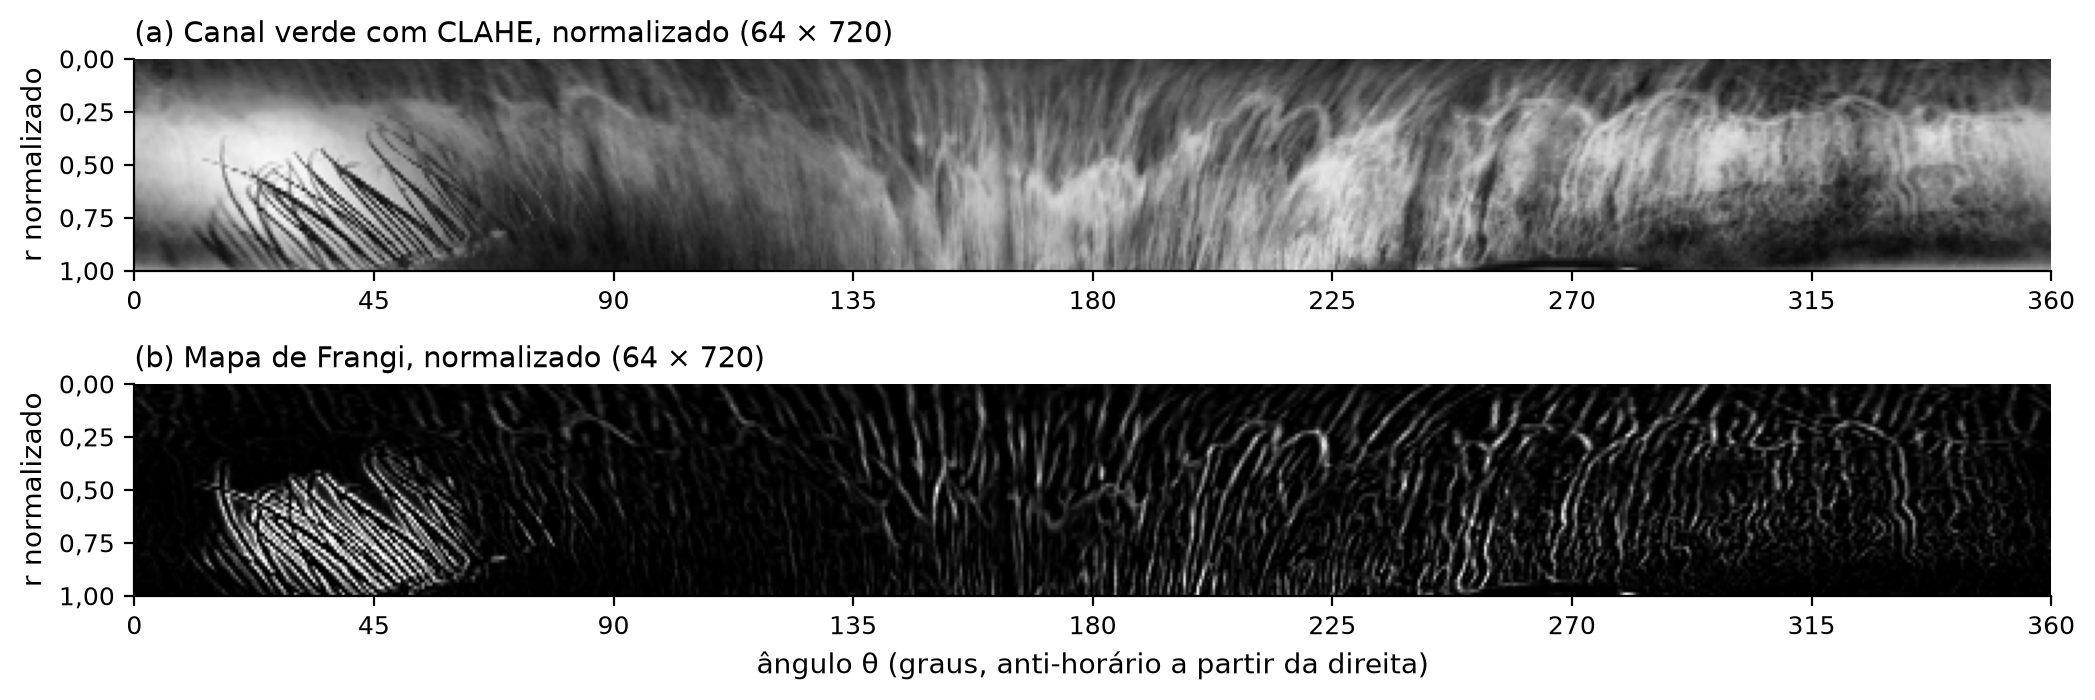
\includegraphics[width=\textwidth]{rubber_sheet_novak.png}
  \fonte{Elaborada pelo autor (2026), a partir de fotografia de
  \citet{Novak2005}.}
\end{figure}

A Figura~\ref{fig:perfil-radial} mostra a fração de pixels de estrutura em
cada raio normalizado. No terço interno do anel, que corresponde
aproximadamente à zona pupilar, essa fração foi de 3,1\% no olho completo e de
3,7\% na macro da íris; nos dois terços externos, de 6,6\% e 8,8\%, isto é,
2,1 e 2,4 vezes maior. Os dois perfis apresentam um mínimo local próximo de
$r \approx 0{,}33$. Uma explicação possível é a coincidência dessa posição com
a do colarete, faixa larga que a escala dominante $\sigma = 1$ não realça; sua
verificação exigiria a marcação do colarete nas imagens. No olho completo, a
fração diminui nas proximidades do limbo, região em que o círculo de Hough não
coincide com o limbo real.

\begin{figure}[htbp]
  \caption{Fração de pixels de estrutura do mapa de Frangi em função do raio
  normalizado (E8)}
  \label{fig:perfil-radial}
  \centering
  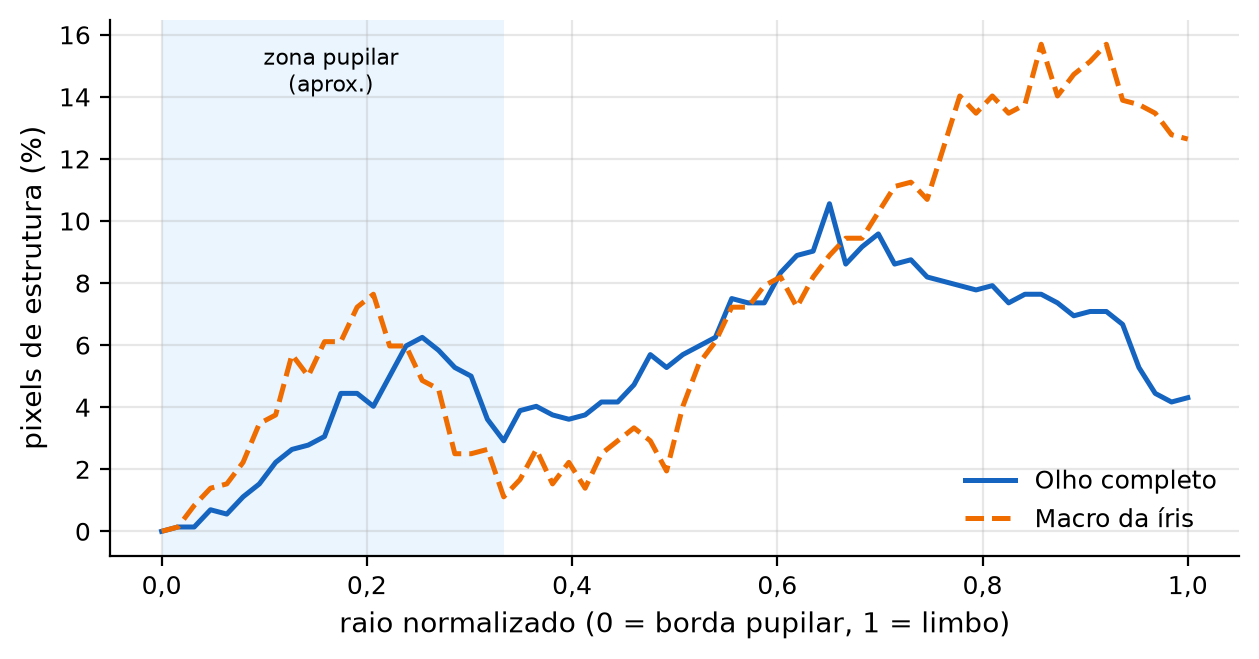
\includegraphics[width=0.75\textwidth]{perfil_radial_frangi.png}
  \fonte{Elaborada pelo autor (2026), a partir de fotografias de
  \citet{Novak2005} e de \citet{Reyes2014}.}
  \nota{A faixa sombreada indica, de forma aproximada, o terço interno do
  anel, sem corresponder a uma delimitação anatômica medida.}
\end{figure}

Como a cadeia de análise já extrai descritores sobre a íris normalizada,
mapas de realce desdobrados dessa forma podem alimentar diretamente
descritores radiais e setoriais de densidade de estruturas, candidatos a
correlatos de vascularização nas próximas etapas.

\secao{Validação da pupila (E9)}
\label{sec:res-pupila}

\subsection{Fotografia do olho completo}

Na fotografia do olho completo (Figura~\ref{fig:pupila-real}), a detecção
encontrou pupila com diâmetro de 162~px e limbo com diâmetro de 402~px, com
anel de 120~px de largura. Os descritores foram $\rho = 0{,}40$,
$\tau = 0{,}60$ e $\epsilon = 0{,}27$, e o validador atribuiu o rótulo
\texttt{valid}, com pontuação 1,00. Com o diâmetro médio da íris como
referência \citep*{Rufer2005}, a escala estimada é de 34,3~px/mm e o diâmetro
pupilar, de aproximadamente 4,7~mm, dentro da faixa de 2 a 8~mm. Duas
ressalvas são necessárias. Primeiro, a Figura~\ref{fig:setores-layout} mostra
que o círculo de Hough está deslocado para a direita e não alcança o limbo
real no lado esquerdo; o diâmetro da íris está, portanto, provavelmente
subestimado, e, em consequência, $\rho$ e a estimativa em milímetros tendem a
estar superestimados. Segundo, a excentricidade de 0,27 encontra-se próxima
do limite de 0,30 e reflete sobretudo esse erro de detecção; um erro
ligeiramente maior alteraria o rótulo para \texttt{borderline}.

\begin{figure}[htbp]
  \caption{Validação da pupila na fotografia do olho completo (E9)}
  \label{fig:pupila-real}
  \centering
  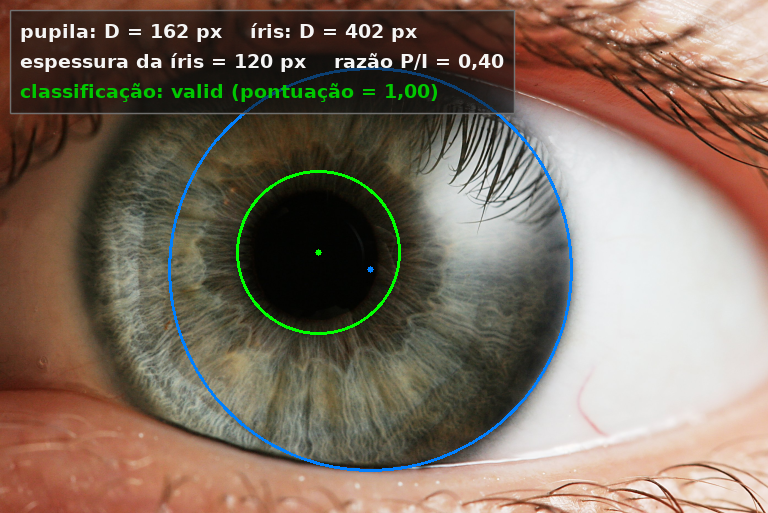
\includegraphics[width=0.74\textwidth]{validacao_pupila_novak.png}
  \fonte{Elaborada pelo autor (2026), a partir de fotografia de
  \citet{Novak2005}.}
  \nota{Pupila em verde e limbo em azul; os descritores e o rótulo aparecem
  na caixa semitransparente.}
\end{figure}

\subsection{Casos sintéticos}

A Tabela~\ref{tab:pupila-sinteticos} apresenta sete geometrias construídas
para percorrer as fronteiras do validador, com raio da íris de 100~px. Os
rótulos seguem as regras do Algoritmo~\ref{alg:validador}: a geometria normal
recebe \texttt{valid}; miose ($\rho = 0{,}18$), midríase moderada
($\rho = 0{,}72$) e excentricidade de 0,40 recebem \texttt{borderline}; miose
extrema ($\rho = 0{,}12$) e anel fino ($\rho = 0{,}88$) violam a faixa
plausível e recebem \texttt{invalid}. A midríase com $\rho = 0{,}78$ situa-se
dentro da faixa plausível, mas acumula duas penalidades (faixa de atenção e
anel com $\tau = 0{,}22$), o que reduz a pontuação a 0,45 e leva ao rótulo
\texttt{invalid}. A Figura~\ref{fig:pupila-curva} mostra a pontuação em função
de $\rho$, e a Figura~\ref{fig:pupila-mapa}, as regiões de decisão no plano
$(\rho, \epsilon)$, nas quais a região \texttt{valid} corresponde ao retângulo
$0{,}20 \le \rho \le 0{,}70$, $\epsilon \le 0{,}30$, e a imagem real se situa
próxima de sua borda superior.

\begin{table}[htbp]
  \caption{Classificação do validador em casos sintéticos (E9)}
  \label{tab:pupila-sinteticos}
  \centering\footnotesize
  % Gerado por experiments/report_experiments.py (não editar à mão).
\begin{tabular}{lccccl}
\toprule
Caso & $\rho$ & $\tau$ & $\epsilon$ & Pontuação & Rótulo \\
\midrule
Normal & 0,40 & 0,60 & 0,00 & 1,00 & \texttt{valid} \\
Miose & 0,18 & 0,82 & 0,00 & 0,75 & \texttt{borderline} \\
Miose extrema & 0,12 & 0,88 & 0,00 & 0,40 & \texttt{invalid} \\
Midríase moderada & 0,72 & 0,28 & 0,00 & 0,75 & \texttt{borderline} \\
Midríase & 0,78 & 0,22 & 0,00 & 0,45 & \texttt{invalid} \\
Excêntrica & 0,40 & 0,60 & 0,40 & 0,70 & \texttt{borderline} \\
Anel fino & 0,88 & 0,12 & 0,00 & 0,10 & \texttt{invalid} \\
\bottomrule
\end{tabular}

  \fonte{Elaborada pelo autor (2026).}
\end{table}

\begin{figure}[htbp]
  \caption{Pontuação do validador em função da razão pupila/íris, com pupila
  centrada (E9)}
  \label{fig:pupila-curva}
  \centering
  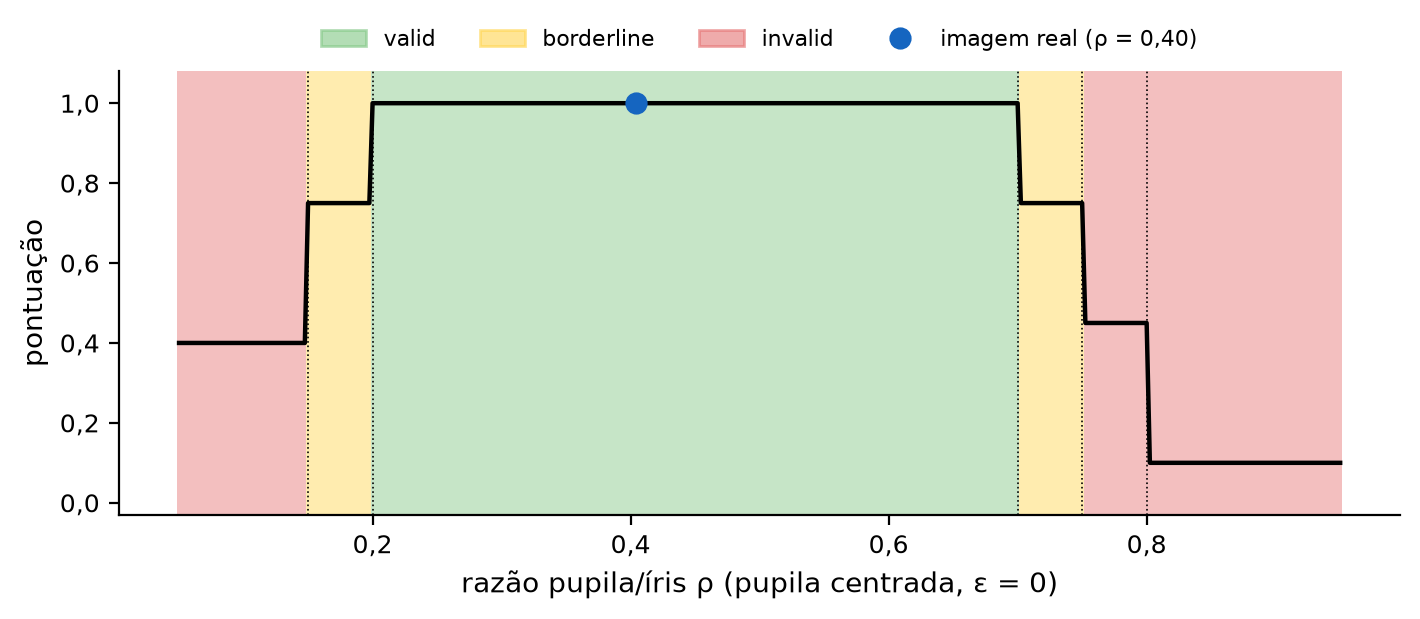
\includegraphics[width=0.85\textwidth]{pupila_curva_pontuacao.png}
  \fonte{Elaborada pelo autor (2026).}
  \nota{As linhas pontilhadas marcam os limites 0,15, 0,20, 0,70, 0,75
  (critério de espessura) e 0,80; o ponto azul representa a imagem real.}
\end{figure}

\begin{figure}[htbp]
  \caption{Regiões de decisão do validador no plano $(\rho, \epsilon)$
  (E9)}
  \label{fig:pupila-mapa}
  \centering
  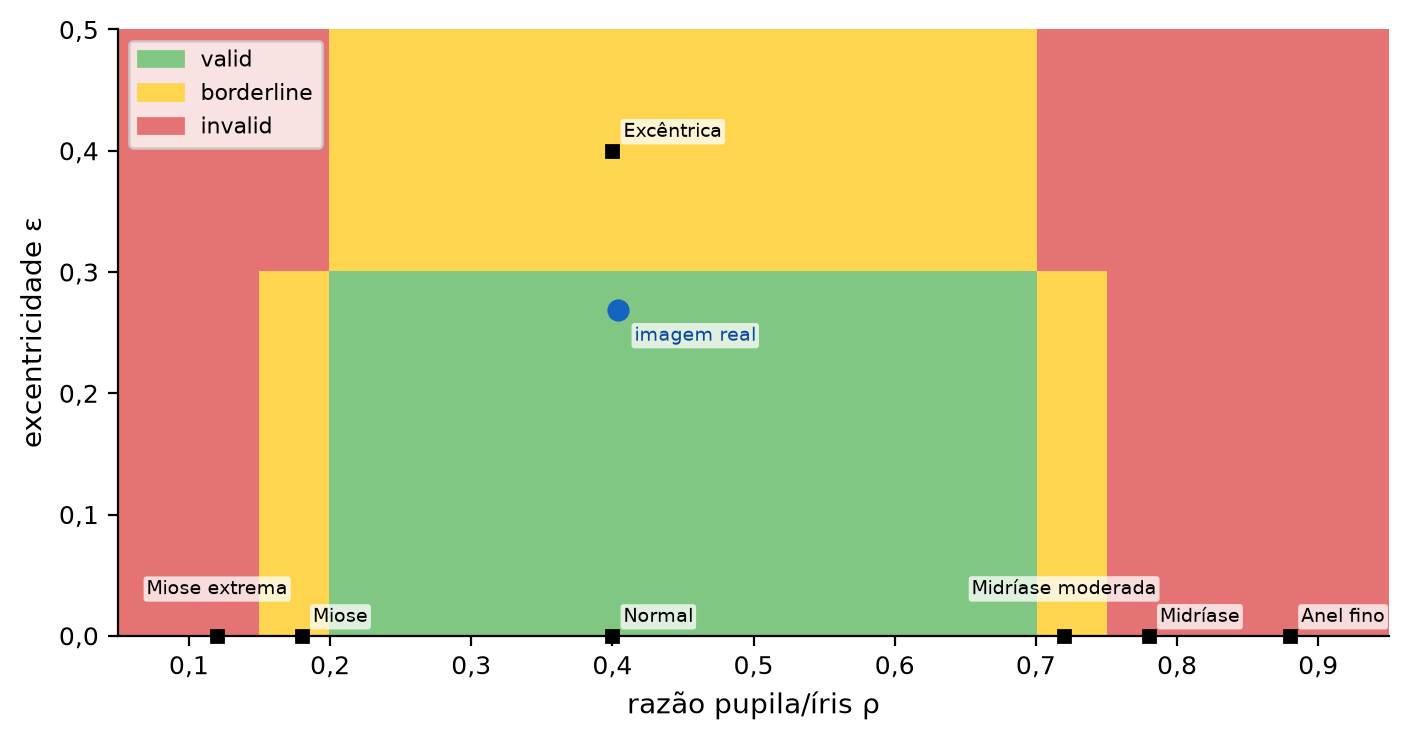
\includegraphics[width=0.85\textwidth]{pupila_mapa_decisao.png}
  \fonte{Elaborada pelo autor (2026).}
  \nota{Quadrados: casos sintéticos; círculo: imagem real.}
\end{figure}

\subsection{Estabilidade da detecção e da validação}

A Tabela~\ref{tab:pupila-estabilidade} apresenta os resultados em 15
condições. Nas sete condições em que a transformada de Hough encontrou o
limbo (original, reduções para 384 e 576~px, rotação, espelhamento, brilho
$+30$ e compressão JPEG), os descritores permaneceram estáveis, com $\rho$
entre 0,36 e 0,41 e $\epsilon$ entre 0,17 e 0,30, todos com rótulo
\texttt{valid}. Na compressão JPEG, contudo, $\epsilon$ atingiu 0,296, a menos
de 0,005 do limite. Nas outras oito condições, o limbo não foi encontrado e o
raio da íris proveio da estimativa de reserva; em duas delas (brilho $-30$ e
correção gama 1,5), a própria pupila também foi estimada. No conjunto, $\rho$
apresentou média de 0,34, desvio-padrão de 0,08 (coeficiente de variação de
23,6\%) e amplitude de 0,17 a 0,41, e 13 das 15 condições receberam o rótulo
\texttt{valid}.

\begin{table}[htbp]
  \caption{Estabilidade da detecção e da validação em 15 condições (E9)}
  \label{tab:pupila-estabilidade}
  \centering\footnotesize
  % Gerado por experiments/report_experiments.py (não editar à mão).
\begin{tabular}{lcccccl}
\toprule
Condição & $D_p$ (px) & $D_i$ (px) & $\rho$ & $\tau$ & $\epsilon$ & Rótulo \\
\midrule
Original (768 px) & 162 & 402 & 0,40 & 0,60 & 0,27 & \texttt{valid} \\
Escala 384 px & 80 & 220 & 0,36 & 0,64 & 0,17 & \texttt{valid} \\
Escala 576 px & 122 & 312 & 0,39 & 0,61 & 0,23 & \texttt{valid} \\
Escala 1152 px & 244 & 739$^\dagger$ & 0,33 & 0,67 & 0,00 & \texttt{valid} \\
Rotação $10^\circ$ & 162 & 406 & 0,40 & 0,60 & 0,26 & \texttt{valid} \\
Espelhamento horizontal & 162 & 404 & 0,40 & 0,60 & 0,27 & \texttt{valid} \\
\midrule
Brilho $-30$ & 82$^\ddagger$ & 492$^\dagger$ & 0,17 & 0,83 & 0,00 & \texttt{borderline} \\
Brilho $+30$ & 162 & 402 & 0,40 & 0,60 & 0,27 & \texttt{valid} \\
Contraste $\times0{,}7$ & 186 & 492$^\dagger$ & 0,38 & 0,62 & 0,00 & \texttt{valid} \\
Contraste $\times1{,}3$ & 153 & 492$^\dagger$ & 0,31 & 0,69 & 0,00 & \texttt{valid} \\
Gama $0{,}7$ & 140 & 492$^\dagger$ & 0,29 & 0,71 & 0,00 & \texttt{valid} \\
Gama $1{,}5$ & 82$^\ddagger$ & 492$^\dagger$ & 0,17 & 0,83 & 0,00 & \texttt{borderline} \\
Ruído gaussiano ($\sigma=8$) & 164 & 492$^\dagger$ & 0,33 & 0,67 & 0,00 & \texttt{valid} \\
Desfoque gaussiano ($\sigma=1{,}5$) & 164 & 492$^\dagger$ & 0,33 & 0,67 & 0,00 & \texttt{valid} \\
Compressão JPEG ($q=30$) & 163 & 394 & 0,41 & 0,59 & 0,30 & \texttt{valid} \\
\bottomrule
\end{tabular}

  \fonte{Elaborada pelo autor (2026).}
  \nota{$\dagger$: raio da íris estimado (limbo não encontrado);
  $\ddagger$: pupila estimada.}
\end{table}

As falhas na detecção da pupila sob escurecimento têm causa identificável.
Com brilho $-30$ e correção gama 1,5, o percentil 3 da imagem aproxima-se de
zero e o limiar do detector passa a 20 e 21 níveis; a máscara escura cresce de
7,0\% da imagem para 18,9\% e 17,3\%, e a maior região escura, que no original
correspondia à pupila (17.662~px$^2$, circularidade 0,85), passa a fundir a
pupila com as partes escuras da íris (62.670 e 57.614~px$^2$, circularidade
0,39 e 0,37). Nenhum candidato atinge a circularidade mínima de 0,55, e o
detector recorre à estimativa. O limiar relativo ao percentil, adequado à
imagem original, torna-se frágil quando o histograma é comprimido nos tons
escuros.

O achado mais relevante para a cadeia de análise, contudo, é outro: o
validador classificou como \texttt{valid} seis condições em que a geometria
foi estimada, e não medida. Nas estimativas de reserva, a íris é centrada na
pupila, o que força $\epsilon = 0$, e, nesta imagem, o raio estimado (48\% do
menor lado) produz valores de $\rho$ dentro da faixa normal. O validador
recebe apenas raios e centros e não tem como distinguir uma geometria medida
de uma geometria preenchida por padrão. Os indicadores de estimativa
produzidos pelo detector precisam, portanto, ser propagados para o validador,
de modo que uma geometria estimada nunca seja classificada como
\texttt{valid}.

% ============================================================================
\chapter{Discussão}
\label{cap:discussao}

\secao{Respostas às questões de pesquisa}
\label{sec:respostas}

Quanto à questão Q1, ajustes de brilho e de contraste não podem aumentar a
separabilidade entre estruturas e fundo (Proposição~1), e os experimentos
confirmaram esse comportamento nas imagens reais e no fantoma. Entre os
realces, o filtro de Frangi produziu o maior ganho, de 2,36 e 2,02 vezes a CNR
da melhor linha de base, superou essa linha de base em todos os 24 setores e
manteve a vantagem quando os setores contaminados pelos cílios foram
excluídos. O banco de Gabor apresentou ganho menor, mas consistente no
conjunto de setores. O realce \bh{}, na configuração padrão, não apresentou
ganho consistente, e seu desempenho depende mais da definição da métrica e das
escalas escolhidas. A resposta a Q1 é, portanto, afirmativa para o filtro de
Frangi e para o banco de Gabor, com a ressalva de que se apoia em duas
imagens.

Quanto à questão Q2, a resposta é parcial. A CNR por Otsu ordenou os métodos
de forma semelhante à AUC no fantoma (correlação de Spearman de 0,76), mas
superestimou o filtro de Frangi sob ruído, porque mapas esparsos separam bem
duas classes mesmo quando parte da estrutura detectada é ruído. Além disso, a
CNR depende da normalização de saída de cada método (E3) e, para alguns
métodos, da região em que o limiar é calculado (E2). A CNR é útil para
comparar métodos em uma mesma imagem sob um protocolo fixo, mas não deve ser
interpretada como medida absoluta de qualidade nem comparada entre
normalizações diferentes. Sempre que houver verdade de referência, ela deve
ser acompanhada da AUC.

Quanto à questão Q3, a variação dos parâmetros não alterou a conclusão
principal: o filtro de Frangi e o banco de Gabor permaneceram acima da melhor
linha de base em todas as configurações testadas. O filtro de Frangi é, no
entanto, o mais sensível ao ruído, ao desfoque e à compressão e, no fantoma,
degradou rapidamente com o ruído, ao passo que o banco de Gabor foi o mais
estável nas duas análises. Os dois resultados têm a mesma origem: na
implementação utilizada, o filtro de Frangi opera quase exclusivamente na
escala mais fina. O custo de todos os métodos é compatível com processamento
em lote.

Quanto à questão Q4, o validador comportou-se conforme projetado nos casos
sintéticos e classificou a imagem real como \texttt{valid}. A cadeia de
detecção e validação, porém, mostrou-se frágil: o limbo não foi encontrado em
8 das 15 condições, e a pupila, em 2. O problema mais grave é que as
estimativas de reserva produzem geometrias plausíveis, aceitas pelo
validador. O validador cumpre seu papel apenas quando recebe medidas reais, de
modo que a robustez da cadeia depende da detecção.

Quanto à questão Q5, os resultados mostram que os métodos funcionam conforme
esperado e permitem compará-los, mas nada revelam sobre o DM2: nenhuma imagem
possui rótulo clínico, e as estruturas realçadas não foram validadas contra a
densidade vascular. As limitações são detalhadas na
Seção~\ref{sec:limitacoes}.

\secao{Implicações para a cadeia de análise}

Os resultados conduzem às seguintes recomendações práticas:
\begin{alineas}
  \item empregar o filtro de Frangi como mapa principal de estruturas finas
  em imagens de boa qualidade e o banco de Gabor como complemento, ou como
  alternativa quando o ruído for relevante, observando que o banco de Gabor
  fornece também a orientação local, útil para descritores de fibras radiais;
  \item normalizar as derivadas do filtro de Frangi pela escala antes de
  utilizar a saída multiescala, para que as fibras mais largas contribuam
  para o mapa;
  \item revisar a configuração morfológica, uma vez que o elemento de 5
  pixels isolado superou a soma de três escalas e que a soma das duas
  polaridades responde a manchas escuras do fundo;
  \item reavaliar o canal de entrada no conjunto rotulado, já que o canal
  azul foi ligeiramente superior ao verde nas duas imagens;
  \item propagar os indicadores de estimativa do detector para o validador,
  rebaixando qualquer geometria estimada, e reduzir a dependência
  fotométrica da detecção do limbo, por exemplo, com normalização de
  contraste antes da transformada de Hough ou com o operador
  integro-diferencial;
  \item medir os descritores de realce sobre a íris normalizada, por setor e
  por raio, excluindo as regiões marcadas como oclusão (cílios e pálpebras).
\end{alineas}

\secao{Limitações e ameaças à validade}
\label{sec:limitacoes}

As principais limitações deste estudo e as ameaças à validade de suas
conclusões são as seguintes:
\begin{alineas}
  \item dados: apenas duas fotografias públicas, sem rótulo clínico, uma
  delas com pós-processamento artístico; os valores-$p$ da análise por
  setores descrevem a consistência dentro de cada imagem, e não a
  generalização para outras íris;
  \item ausência do conjunto rotulado: o conjunto rotulado para DM2 não
  estava disponível nesta etapa, de modo que nenhuma associação com a doença
  foi testada;
  \item modalidade: fotografias RGB não medem fluxo nem densidade vascular,
  e as estruturas realçadas incluem trabéculas, bordas de criptas e, em
  parte, vasos;
  \item métrica: a CNR por Otsu depende da normalização de saída, da região
  do limiar e do nível de ruído e favorece mapas esparsos, ao passo que a AUC
  foi medida apenas no fantoma;
  \item fantoma: o modelo emprega curvas claras de 1 a 3 pixels, ruído
  gaussiano e textura suave, sem reproduzir reflexos, cílios, pálpebras,
  artefatos de compressão ou estruturas escuras, como criptas;
  \item detecção: o detector utiliza limiares fixos e heurísticos, a
  transformada de Hough mostrou-se sensível à escala e à fotometria, e as
  estimativas de reserva produzem geometrias de aparência plausível;
  \item validador: as faixas de $\rho$ derivam de valores populacionais
  publicados, enquanto o limite de excentricidade e as penalidades constituem
  escolhas de projeto, não ajustadas a dados;
  \item parâmetros: a configuração padrão não foi otimizada, e há
  configurações com CNR maior, cujo ajuste exige dados separados dos
  utilizados na avaliação;
  \item tempo de execução: os tempos dependem da máquina e da carga, de modo
  que apenas a ordem relativa entre os métodos deve ser generalizada.
\end{alineas}

% ============================================================================
\chapter{Conclusão e trabalhos futuros}
\label{cap:conclusao}

Esta etapa cumpriu as duas metas definidas ao término do PGC~I. Três
algoritmos consolidados de realce de estruturas finas, a saber, o filtro de
Frangi, o banco de filtros de Gabor e a morfologia \tht{}/\bh{}, foram
integrados à cadeia de análise e avaliados por um protocolo reprodutível de
onze experimentos, e um validador da geometria pupila--íris baseado em faixas
fisiológicas foi implementado e testado. O filtro de Frangi foi o realce com
maior separação entre estruturas e fundo nas imagens reais, com vantagem
consistente entre regiões da íris. O banco de Gabor apresentou ganho menor,
mas foi o mais estável sob ruído, desfoque e compressão e o melhor no fantoma
com ruído moderado ou alto. O validador classificou corretamente os casos
sintéticos e a imagem real.

Três lições metodológicas orientam as próximas etapas. A primeira é que
ajustes de brilho e de contraste não podem, por construção, tornar estruturas
mais separáveis do fundo e, por isso, não constituem linha de base suficiente
para o realce. A segunda é que a métrica sem verdade de referência precisa ser
interpretada com cautela, pois depende da normalização de saída e superestima
mapas esparsos sob ruído. A terceira é que a vulnerabilidade da validação
geométrica não reside nas regras de classificação, mas na detecção do limbo e
no tratamento das estimativas de reserva.

Como trabalhos futuros, propõe-se:
\begin{alineas}
  \item aplicar os realces ao conjunto rotulado para DM2, sob particionamento
  \emph{person-based}, extraindo descritores de densidade de estruturas por
  setor e por raio sobre a íris normalizada, e testar sua associação com o
  rótulo em comparação com a linha de base da cadeia de análise;
  \item normalizar as derivadas do filtro de Frangi pela escala
  \citep*{Lindeberg1998} e avaliar a variante proposta por
  \citet{Jerman2016};
  \item ajustar parâmetros como $\beta$, $\lambda$, as escalas morfológicas e
  o canal de entrada em dados de ajuste separados dos dados de teste;
  \item anotar manualmente as estruturas finas em um pequeno conjunto de
  imagens da íris, de modo a medir a AUC em imagens reais;
  \item reduzir a sensibilidade da detecção à fotometria e à escala, com
  normalização de contraste antes da transformada de Hough, operador
  integro-diferencial \citep*{Daugman2004} ou contornos ativos
  \citep*{Kass1988}, e propagar os indicadores de estimativa para o
  validador;
  \item aprender os limiares do validador a partir de dados com rótulo de
  qualidade, utilizando o vetor de descritores que ele já fornece;
  \item calibrar a escala em milímetros quando a resolução ou a distância de
  aquisição forem conhecidas, de modo a aproximar o diâmetro pupilar
  absoluto, biomarcador candidato do DM2 \citep*{Cui2024,Thakar2025}.
\end{alineas}

Em síntese, os resultados desta etapa indicam que fotografias RGB
convencionais permitem realçar, de forma reprodutível, estruturas finas do
estroma iridiano e verificar a plausibilidade da geometria pupila--íris.
Essas condições são necessárias, mas não suficientes, para a extração de
correlatos de biomarcadores oculares do DM2: a existência de associação entre
os descritores derivados dos realces e o diagnóstico permanece uma hipótese,
cuja verificação depende da aplicação dos métodos ao conjunto rotulado e
constitui o foco da próxima etapa do projeto.

% ============================================================================
\postextual

\begin{thebibliography}{99}

\bibitem[Abràmoff, Garvin e Sonka(2010)Abràmoff; Garvin; Sonka]{Abramoff2010}
ABRÀMOFF, M. D.; GARVIN, M. K.; SONKA, M. Retinal imaging and image analysis.
\textbf{IEEE Reviews in Biomedical Engineering}, \semlocal, v. 3, p. 169-208,
2010. \doi{10.1109/RBME.2010.2084567}.

\bibitem[Bowyer, Hollingsworth e Flynn(2008)Bowyer; Hollingsworth; Flynn]{Bowyer2008}
BOWYER, K. W.; HOLLINGSWORTH, K.; FLYNN, P. J. Image understanding for iris
biometrics: a survey. \textbf{Computer Vision and Image Understanding},
\semlocal, v. 110, n. 2, p. 281-307, 2008. \doi{10.1016/j.cviu.2007.08.005}.

\bibitem[Bradski(2000)]{Bradski2000}
BRADSKI, G. The OpenCV library. \textbf{Dr. Dobb's Journal of Software
Tools}, \semlocal, 2000.

\bibitem[Chaudhuri et~al.(1989)]{Chaudhuri1989}
CHAUDHURI, S.; CHATTERJEE, S.; KATZ, N.; NELSON, M.; GOLDBAUM, M. Detection
of blood vessels in retinal images using two-dimensional matched filters.
\textbf{IEEE Transactions on Medical Imaging}, \semlocal, v. 8, n. 3,
p. 263-269, 1989. \doi{10.1109/42.34715}.

\bibitem[Cui et~al.(2024)]{Cui2024}
CUI, L.; XIAO, Y.; XIANG, Z.; CHEN, Z.; YANG, C.; ZOU, H. Study on the
correlation between iris blood flow, iris thickness and pupil diameter in the
resting state and after pharmacological mydriasis in patients with diabetes
mellitus. \textbf{BMC Ophthalmology}, \semlocal, v. 24, n. 1, art. 52, 2024.
\doi{10.1186/s12886-024-03322-y}.

\bibitem[Daugman(1985)]{Daugman1985}
DAUGMAN, J. G. Uncertainty relation for resolution in space, spatial
frequency, and orientation optimized by two-dimensional visual cortical
filters. \textbf{Journal of the Optical Society of America A}, \semlocal,
v. 2, n. 7, p. 1160-1169, 1985. \doi{10.1364/JOSAA.2.001160}.

\bibitem[Daugman(1993)]{Daugman1993}
DAUGMAN, J. G. High confidence visual recognition of persons by a test of
statistical independence. \textbf{IEEE Transactions on Pattern Analysis and
Machine Intelligence}, \semlocal, v. 15, n. 11, p. 1148-1161, 1993.
\doi{10.1109/34.244676}.

\bibitem[Daugman(2004)]{Daugman2004}
DAUGMAN, J. How iris recognition works. \textbf{IEEE Transactions on Circuits
and Systems for Video Technology}, \semlocal, v. 14, n. 1, p. 21-30, 2004.
\doi{10.1109/TCSVT.2003.818350}.

\bibitem[Dice(1945)]{Dice1945}
DICE, L. R. Measures of the amount of ecologic association between species.
\textbf{Ecology}, \semlocal, v. 26, n. 3, p. 297-302, 1945.
\doi{10.2307/1932409}.

\bibitem[Duda e Hart(1972)Duda; Hart]{DudaHart1972}
DUDA, R. O.; HART, P. E. Use of the Hough transformation to detect lines and
curves in pictures. \textbf{Communications of the ACM}, \semlocal, v. 15,
n. 1, p. 11-15, 1972. \doi{10.1145/361237.361242}.

\bibitem[Efron(1979)]{Efron1979}
EFRON, B. Bootstrap methods: another look at the jackknife. \textbf{The
Annals of Statistics}, \semlocal, v. 7, n. 1, p. 1-26, 1979.
\doi{10.1214/aos/1176344552}.

\bibitem[Ernst(2000)]{Ernst2000}
ERNST, E. Iridology: not useful and potentially harmful. \textbf{Archives of
Ophthalmology}, \semlocal, v. 118, n. 1, p. 120-121, 2000.
\doi{10.1001/archopht.118.1.120}.

\bibitem[Fawcett(2006)]{Fawcett2006}
FAWCETT, T. An introduction to ROC analysis. \textbf{Pattern Recognition
Letters}, \semlocal, v. 27, n. 8, p. 861-874, 2006.
\doi{10.1016/j.patrec.2005.10.010}.

\bibitem[Frangi et~al.(1998)]{Frangi1998}
FRANGI, A. F.; NIESSEN, W. J.; VINCKEN, K. L.; VIERGEVER, M. A. Multiscale
vessel enhancement filtering. In: INTERNATIONAL CONFERENCE ON MEDICAL IMAGE
COMPUTING AND COMPUTER-ASSISTED INTERVENTION, 1., 1998, Cambridge.
\textbf{Proceedings} [\dots]. Berlin: Springer, 1998. p. 130-137. (Lecture
Notes in Computer Science, v. 1496). \doi{10.1007/BFb0056195}.

\bibitem[Fraz et~al.(2012)]{Fraz2012}
FRAZ, M. M.; REMAGNINO, P.; HOPPE, A.; UYYANONVARA, B.; RUDNICKA, A. R.;
OWEN, C. G.; BARMAN, S. A. Blood vessel segmentation methodologies in retinal
images: a survey. \textbf{Computer Methods and Programs in Biomedicine},
\semlocal, v. 108, n. 1, p. 407-433, 2012. \doi{10.1016/j.cmpb.2012.03.009}.

\bibitem[Gabor(1946)]{Gabor1946}
GABOR, D. Theory of communication. Part 1: the analysis of information.
\textbf{Journal of the Institution of Electrical Engineers - Part III: Radio
and Communication Engineering}, \semlocal, v. 93, n. 26, p. 429-441, 1946.
\doi{10.1049/ji-3-2.1946.0074}.

\bibitem[Gonzalez e Woods(2018)Gonzalez; Woods]{GonzalezWoods2018}
GONZALEZ, R. C.; WOODS, R. E. \textbf{Digital image processing}. 4. ed. New
York: Pearson, 2018.

\bibitem[Gulshan et~al.(2016)]{Gulshan2016}
GULSHAN, V. et al. Development and validation of a deep learning algorithm
for detection of diabetic retinopathy in retinal fundus photographs.
\textbf{JAMA}, \semlocal, v. 316, n. 22, p. 2402-2410, 2016.
\doi{10.1001/jama.2016.17216}.

\bibitem[Hanley e McNeil(1982)Hanley; McNeil]{HanleyMcNeil1982}
HANLEY, J. A.; MCNEIL, B. J. The meaning and use of the area under a receiver
operating characteristic (ROC) curve. \textbf{Radiology}, \semlocal, v. 143,
n. 1, p. 29-36, 1982. \doi{10.1148/radiology.143.1.7063747}.

\bibitem[Harris et~al.(2020)]{Harris2020}
HARRIS, C. R. et al. Array programming with NumPy. \textbf{Nature},
\semlocal, v. 585, n. 7825, p. 357-362, 2020.
\doi{10.1038/s41586-020-2649-2}.

\bibitem[Hoover, Kouznetsova e Goldbaum(2000)Hoover; Kouznetsova; Goldbaum]{Hoover2000}
HOOVER, A. D.; KOUZNETSOVA, V.; GOLDBAUM, M. Locating blood vessels in
retinal images by piecewise threshold probing of a matched filter response.
\textbf{IEEE Transactions on Medical Imaging}, \semlocal, v. 19, n. 3,
p. 203-210, 2000. \doi{10.1109/42.845178}.

\bibitem[Hunter(2007)]{Hunter2007}
HUNTER, J. D. Matplotlib: a 2D graphics environment. \textbf{Computing in
Science \& Engineering}, \semlocal, v. 9, n. 3, p. 90-95, 2007.
\doi{10.1109/MCSE.2007.55}.

\bibitem[Jain e Farrokhnia(1991)Jain; Farrokhnia]{Jain1991}
JAIN, A. K.; FARROKHNIA, F. Unsupervised texture segmentation using Gabor
filters. \textbf{Pattern Recognition}, \semlocal, v. 24, n. 12,
p. 1167-1186, 1991. \doi{10.1016/0031-3203(91)90143-S}.

\bibitem[Jerman et~al.(2016)]{Jerman2016}
JERMAN, T.; PERNUŠ, F.; LIKAR, B.; ŠPICLIN, Ž. Enhancement of vascular
structures in 3D and 2D angiographic images. \textbf{IEEE Transactions on
Medical Imaging}, \semlocal, v. 35, n. 9, p. 2107-2118, 2016.
\doi{10.1109/TMI.2016.2550102}.

\bibitem[Kass, Witkin e Terzopoulos(1988)Kass; Witkin; Terzopoulos]{Kass1988}
KASS, M.; WITKIN, A.; TERZOPOULOS, D. Snakes: active contour models.
\textbf{International Journal of Computer Vision}, \semlocal, v. 1, n. 4,
p. 321-331, 1988. \doi{10.1007/BF00133570}.

\bibitem[Koenderink(1984)]{Koenderink1984}
KOENDERINK, J. J. The structure of images. \textbf{Biological Cybernetics},
\semlocal, v. 50, n. 5, p. 363-370, 1984. \doi{10.1007/BF00336961}.

\bibitem[Lindeberg(1998)]{Lindeberg1998}
LINDEBERG, T. Edge detection and ridge detection with automatic scale
selection. \textbf{International Journal of Computer Vision}, \semlocal,
v. 30, n. 2, p. 117-156, 1998. \doi{10.1023/A:1008097225773}.

\bibitem[Mendonça e Campilho(2006)Mendonça; Campilho]{Mendonca2006}
MENDONÇA, A. M.; CAMPILHO, A. Segmentation of retinal blood vessels by
combining the detection of centerlines and morphological reconstruction.
\textbf{IEEE Transactions on Medical Imaging}, \semlocal, v. 25, n. 9,
p. 1200-1213, 2006. \doi{10.1109/TMI.2006.879955}.

\bibitem[Novák(2005)]{Novak2005}
NOVÁK, P. \textbf{Eye iris}. 2005. 1 fotografia, color. Licença CC BY-SA 2.5.
Disponível em: \url{https://commons.wikimedia.org/wiki/File:Eye_iris.jpg}.
Acesso em: 7 out. 2026.

\bibitem[Otsu(1979)]{Otsu1979}
OTSU, N. A threshold selection method from gray-level histograms.
\textbf{IEEE Transactions on Systems, Man, and Cybernetics}, \semlocal, v. 9,
n. 1, p. 62-66, 1979. \doi{10.1109/TSMC.1979.4310076}.

\bibitem[Pech-Pacheco et~al.(2000)]{PechPacheco2000}
PECH-PACHECO, J. L.; CRISTÓBAL, G.; CHAMORRO-MARTÍNEZ, J.;
FERNÁNDEZ-VALDIVIA, J. Diatom autofocusing in brightfield microscopy: a
comparative study. In: INTERNATIONAL CONFERENCE ON PATTERN RECOGNITION, 15.,
2000, Barcelona. \textbf{Proceedings} [\dots]. Los Alamitos: IEEE Computer
Society, 2000. v. 3, p. 314-317. \doi{10.1109/ICPR.2000.903548}.

\bibitem[Pedregosa et~al.(2011)]{Pedregosa2011}
PEDREGOSA, F. et al. Scikit-learn: machine learning in Python.
\textbf{Journal of Machine Learning Research}, \semlocal, v. 12, n. 85,
p. 2825-2830, 2011. Disponível em:
\url{https://jmlr.org/papers/v12/pedregosa11a.html}. Acesso em: 7 out. 2026.

\bibitem[Pizer et~al.(1987)]{Pizer1987}
PIZER, S. M.; AMBURN, E. P.; AUSTIN, J. D.; CROMARTIE, R.; GESELOWITZ, A.;
GREER, T.; TER HAAR ROMENY, B.; ZIMMERMAN, J. B.; ZUIDERVELD, K. Adaptive
histogram equalization and its variations. \textbf{Computer Vision, Graphics,
and Image Processing}, \semlocal, v. 39, n. 3, p. 355-368, 1987.
\doi{10.1016/S0734-189X(87)80186-X}.

\bibitem[Reyes(2014)]{Reyes2014}
REYES, C. A. \textbf{Iris eclipse - Explored}. 2014. 1 fotografia, color.
Licença CC BY 2.0. Disponível em:
\url{https://commons.wikimedia.org/wiki/File:Iris_eclipse_-_Explored_-_Flickr_-_creyesk.jpg}.
Acesso em: 7 out. 2026.

\bibitem[Ricci e Perfetti(2007)Ricci; Perfetti]{RicciPerfetti2007}
RICCI, E.; PERFETTI, R. Retinal blood vessel segmentation using line
operators and support vector classification. \textbf{IEEE Transactions on
Medical Imaging}, \semlocal, v. 26, n. 10, p. 1357-1365, 2007.
\doi{10.1109/TMI.2007.898551}.

\bibitem[Roberts, Goldstein e Fawzi(2017)Roberts; Goldstein; Fawzi]{Roberts2017}
ROBERTS, P. K.; GOLDSTEIN, D. A.; FAWZI, A. A. Anterior segment optical
coherence tomography angiography for identification of iris vasculature and
staging of iris neovascularization: a pilot study. \textbf{Current Eye
Research}, \semlocal, v. 42, n. 8, p. 1136-1142, 2017.
\doi{10.1080/02713683.2017.1293113}.

\bibitem[Rüfer, Schröder e Erb(2005)Rüfer; Schröder; Erb]{Rufer2005}
RÜFER, F.; SCHRÖDER, A.; ERB, C. White-to-white corneal diameter: normal
values in healthy humans obtained with the Orbscan II topography system.
\textbf{Cornea}, \semlocal, v. 24, n. 3, p. 259-261, 2005.
\doi{10.1097/01.ico.0000148312.01805.53}.

\bibitem[Samant e Agarwal(2018)Samant; Agarwal]{SamantAgarwal2018}
SAMANT, P.; AGARWAL, R. Machine learning techniques for medical diagnosis of
diabetes using iris images. \textbf{Computer Methods and Programs in
Biomedicine}, \semlocal, v. 157, p. 121-128, 2018.
\doi{10.1016/j.cmpb.2018.01.004}.

\bibitem[Sato et~al.(1998)]{Sato1998}
SATO, Y.; NAKAJIMA, S.; SHIRAGA, N.; ATSUMI, H.; YOSHIDA, S.; KOLLER, T.;
GERIG, G.; KIKINIS, R. Three-dimensional multi-scale line filter for
segmentation and visualization of curvilinear structures in medical images.
\textbf{Medical Image Analysis}, \semlocal, v. 2, n. 2, p. 143-168, 1998.
\doi{10.1016/S1361-8415(98)80009-1}.

\bibitem[Shannon(1948)]{Shannon1948}
SHANNON, C. E. A mathematical theory of communication. \textbf{Bell System
Technical Journal}, \semlocal, v. 27, n. 3, p. 379-423, 1948.
\doi{10.1002/j.1538-7305.1948.tb01338.x}.

\bibitem[Simon, Worthen e Mitas(1979)Simon; Worthen; Mitas]{Simon1979}
SIMON, A.; WORTHEN, D. M.; MITAS, J. A. An evaluation of iridology.
\textbf{JAMA}, \semlocal, v. 242, n. 13, p. 1385-1389, 1979.
\doi{10.1001/jama.1979.03300130029014}.

\bibitem[Soares et~al.(2006)]{Soares2006}
SOARES, J. V. B.; LEANDRO, J. J. G.; CESAR JUNIOR, R. M.; JELINEK, H. F.;
CREE, M. J. Retinal vessel segmentation using the 2-D Gabor wavelet and
supervised classification. \textbf{IEEE Transactions on Medical Imaging},
\semlocal, v. 25, n. 9, p. 1214-1222, 2006. \doi{10.1109/TMI.2006.879967}.

\bibitem[Soille(2004)]{Soille2004}
SOILLE, P. \textbf{Morphological image analysis}: principles and
applications. 2. ed. Berlin: Springer, 2004.
\doi{10.1007/978-3-662-05088-0}.

\bibitem[Spearman(1904)]{Spearman1904}
SPEARMAN, C. The proof and measurement of association between two things.
\textbf{The American Journal of Psychology}, \semlocal, v. 15, n. 1,
p. 72-101, 1904. \doi{10.2307/1412159}.

\bibitem[Staal et~al.(2004)]{Staal2004}
STAAL, J.; ABRÀMOFF, M. D.; NIEMEIJER, M.; VIERGEVER, M. A.; VAN GINNEKEN, B.
Ridge-based vessel segmentation in color images of the retina. \textbf{IEEE
Transactions on Medical Imaging}, \semlocal, v. 23, n. 4, p. 501-509, 2004.
\doi{10.1109/TMI.2004.825627}.

\bibitem[Surya et~al.(2026)]{Surya2026}
SURYA, J.; TAMILSELVI, S.; ROY, M.; CHINNASAMY, S.; RAMAN, R.; SUCHETHA, M.;
RAJENDRAN, G. Machine learning-based prediction of diabetic retinopathy from
pupillary abnormalities in a South Indian population. \textbf{PLOS One},
\semlocal, v. 21, n. 1, e0340802, 2026. \doi{10.1371/journal.pone.0340802}.

\bibitem[Thakar et~al.(2025)]{Thakar2025}
THAKAR, M.; TRIPATHY, S. P.; DUTTA, P.; BHATTACHARYA, S.; DHAKA, U.
Quantitative automated pupillometry in diabetic patients and correlation with
retinal nerve fibre layer thickness. \textbf{Eye}, \semlocal, v. 39, n. 10,
p. 1983-1989, 2025. \doi{10.1038/s41433-025-03793-3}.

\bibitem[van der Walt et~al.(2014)]{vanderWalt2014}
VAN DER WALT, S.; SCHÖNBERGER, J. L.; NUNEZ-IGLESIAS, J.; BOULOGNE, F.;
WARNER, J. D.; YAGER, N.; GOUILLART, E.; YU, T. scikit-image: image
processing in Python. \textbf{PeerJ}, \semlocal, v. 2, e453, 2014.
\doi{10.7717/peerj.453}.

\bibitem[Virtanen et~al.(2020)]{Virtanen2020}
VIRTANEN, P. et al. SciPy 1.0: fundamental algorithms for scientific
computing in Python. \textbf{Nature Methods}, \semlocal, v. 17, n. 3,
p. 261-272, 2020. \doi{10.1038/s41592-019-0686-2}.

\bibitem[Watson e Yellott(2012)Watson; Yellott]{WatsonYellott2012}
WATSON, A. B.; YELLOTT, J. I. A unified formula for light-adapted pupil size.
\textbf{Journal of Vision}, \semlocal, v. 12, n. 10, art. 12, 2012.
\doi{10.1167/12.10.12}.

\bibitem[Welvaert e Rosseel(2013)Welvaert; Rosseel]{Welvaert2013}
WELVAERT, M.; ROSSEEL, Y. On the definition of signal-to-noise ratio and
contrast-to-noise ratio for fMRI data. \textbf{PLoS ONE}, \semlocal, v. 8,
n. 11, e77089, 2013. \doi{10.1371/journal.pone.0077089}.

\bibitem[Wilcoxon(1945)]{Wilcoxon1945}
WILCOXON, F. Individual comparisons by ranking methods. \textbf{Biometrics
Bulletin}, \semlocal, v. 1, n. 6, p. 80-83, 1945. \doi{10.2307/3001968}.

\bibitem[Wildes(1997)]{Wildes1997}
WILDES, R. P. Iris recognition: an emerging biometric technology.
\textbf{Proceedings of the IEEE}, \semlocal, v. 85, n. 9, p. 1348-1363, 1997.
\doi{10.1109/5.628669}.

\bibitem[Zana e Klein(2001)Zana; Klein]{ZanaKlein2001}
ZANA, F.; KLEIN, J.-C. Segmentation of vessel-like patterns using
mathematical morphology and curvature evaluation. \textbf{IEEE Transactions
on Image Processing}, \semlocal, v. 10, n. 7, p. 1010-1019, 2001.
\doi{10.1109/83.931095}.

\bibitem[Zech et~al.(2018)]{Zech2018}
ZECH, J. R.; BADGELEY, M. A.; LIU, M.; COSTA, A. B.; TITANO, J. J.;
OERMANN, E. K. Variable generalization performance of a deep learning model
to detect pneumonia in chest radiographs: a cross-sectional study.
\textbf{PLOS Medicine}, \semlocal, v. 15, n. 11, e1002683, 2018.
\doi{10.1371/journal.pmed.1002683}.

\bibitem[Zett et~al.(2018)]{Zett2018}
ZETT, C.; STINA, D. M. R.; KATO, R. T.; NOVAIS, E. A.; ALLEMANN, N.
Comparison of anterior segment optical coherence tomography angiography and
fluorescein angiography for iris vasculature analysis. \textbf{Graefe's
Archive for Clinical and Experimental Ophthalmology}, \semlocal, v. 256,
n. 4, p. 683-691, 2018. \doi{10.1007/s00417-018-3935-7}.

\bibitem[Zhou et~al.(2025)]{Zhou2025}
ZHOU, Y.; WANG, T.; GUO, Z.; SHE, F.; ZENG, J.; ZHU, X. Assessment of iris
vasculature in type 2 diabetes mellitus patients without diabetic retinopathy
using anterior segment optical coherence tomography angiography.
\textbf{Scientific Reports}, \semlocal, v. 15, n. 1, art. 19035, 2025.
\doi{10.1038/s41598-025-04463-w}.

\bibitem[Zhu et~al.(2026)]{Zhu2026}
ZHU, Y.; SUN, S.; HAN, S.; CHEN, J.; WESTERN, D.; ZHANG, L. Automated method
for quantitative analysis of iris fluorescein angiography based on machine
learning. \textbf{Quantitative Imaging in Medicine and Surgery}, \semlocal,
v. 16, n. 1, p. 68, 2026. \doi{10.21037/qims-2025-480}.

\bibitem[Zuiderveld(1994)]{Zuiderveld1994}
ZUIDERVELD, K. Contrast limited adaptive histogram equalization. In:
HECKBERT, P. S. (ed.). \textbf{Graphics gems IV}. Boston: AP Professional,
1994. p. 474-485. \doi{10.1016/B978-0-12-336156-1.50061-6}.

\end{thebibliography}

% ============================================================================
\begin{apendicesenv}

\chapter{Reprodutibilidade}
\label{ap:repro}

Os comandos a seguir, executados a partir da raiz do repositório em
PowerShell, reproduzem todos os resultados, executam os testes e compilam
este documento. O \emph{script} de experimentos demanda cerca de três minutos
na máquina descrita no Quadro~\ref{qua:ambiente}.

\begin{SingleSpace}
\begin{verbatim}
.\.venv\Scripts\python.exe experiments\report_experiments.py
.\.venv\Scripts\python.exe -m unittest discover -s tests
cd docs\PGC_2
pdflatex metodologia_vascularizacao_pupila.tex
pdflatex metodologia_vascularizacao_pupila.tex
\end{verbatim}
\end{SingleSpace}

\begin{quadro}[htbp]
  \caption{Ambiente de execução dos experimentos}
  \label{qua:ambiente}
  \footnotesize
  \renewcommand{\arraystretch}{1.15}
  \begin{tabular}{|l|l|}
    \hline
    \textbf{Componente} & \textbf{Versão ou descrição} \\ \hline
    Python & 3.12.10 \\ \hline
    NumPy & 2.5.3 \\ \hline
    OpenCV & 5.0.0 \\ \hline
    scikit-image & 0.26.0 \\ \hline
    SciPy & 1.18.1 \\ \hline
    scikit-learn & 1.9.1 \\ \hline
    Matplotlib & 3.11.2 \\ \hline
    Sistema operacional & Windows 11 (versão 10.0.26300) \\ \hline
    Processador & Intel Core i7-1270P (12.ª geração), 31,6~GB de memória \\ \hline
  \end{tabular}
  \fonte{Elaborado pelo autor (2026).}
\end{quadro}

As fontes de aleatoriedade são controladas por sementes fixas: semente 0 no
\emph{bootstrap} da análise por setores e no ruído da perturbação dos
experimentos E5 e E9, e sementes 0 a 9 nos fantomas. O
Quadro~\ref{qua:arquivos} relaciona cada experimento aos arquivos que ele
gera.

\begin{quadro}[htbp]
  \caption{Arquivos gerados por experimento no diretório
  \arq{docs/PGC_2}}
  \label{qua:arquivos}
  \footnotesize
  \renewcommand{\arraystretch}{1.15}
  \begin{tabular}{|>{\raggedright\arraybackslash}p{2.0cm}
                  |>{\raggedright\arraybackslash}p{12.2cm}|}
    \hline
    \textbf{Experimento} & \textbf{Arquivos} \\ \hline
    Metodologia & \arq{figuras/banco_gabor.png}, \arq{figuras/clahe_novak.png},
      \arq{figuras/setores_layout_novak.png} \\ \hline
    E0 & \arq{tabelas/tab_vasc_principal.tex}, \arq{dados/cnr_principal.dat},
      \arq{figuras/painel_vascularizacao_novak.png},
      \arq{figuras/painel_vascularizacao_closeup.png},
      \arq{figuras/histograma_estrutura_fundo.png},
      \arq{figuras/detalhe_estroma_closeup.png} \\ \hline
    E1 & \arq{tabelas/tab_setores.tex}, \arq{figuras/setores_cnr_boxplot.png},
      \arq{figuras/setores_polar.png} \\ \hline
    E2 & \arq{tabelas/tab_metrica_otsu.tex} \\ \hline
    E3 & \arq{tabelas/tab_frangi_escalas.tex},
      \arq{tabelas/tab_frangi_normalizacao.tex},
      \arq{figuras/frangi_escalas_closeup.png} \\ \hline
    E4 & \arq{tabelas/tab_sensibilidade.tex} \\ \hline
    E5 & \arq{tabelas/tab_robustez.tex}, \arq{figuras/robustez_frangi_exemplo.png} \\ \hline
    E6 & \arq{tabelas/tab_fantoma.tex}, \arq{dados/auc_ruido.dat},
      \arq{figuras/fantoma_exemplo.png}, \arq{figuras/fantoma_roc.png} \\ \hline
    E7 & \arq{tabelas/tab_tempo.tex} \\ \hline
    E8 & \arq{figuras/rubber_sheet_novak.png}, \arq{figuras/perfil_radial_frangi.png},
      \arq{dados/perfil_radial_novak.dat}, \arq{dados/perfil_radial_closeup.dat} \\ \hline
    E9 & \arq{figuras/validacao_pupila_novak.png},
      \arq{figuras/pupila_curva_pontuacao.png},
      \arq{figuras/pupila_mapa_decisao.png},
      \arq{tabelas/tab_pupila_sinteticos.tex},
      \arq{tabelas/tab_pupila_estabilidade.tex} \\ \hline
    E10 & \arq{tabelas/tab_canais.tex} \\ \hline
  \end{tabular}
  \fonte{Elaborado pelo autor (2026).}
\end{quadro}

\chapter{Configuração completa}
\label{ap:config}

O Quadro~\ref{qua:config-completa} reúne os valores utilizados pelo realce,
pelo detector, pelo validador e pelos experimentos. Os valores do realce e do
validador encontram-se em \arq{src/config.py}; os do detector, em
\arq{experiments/demo_vascularization_pupil.py}; e os dos experimentos, em
\arq{experiments/report_experiments.py}.

\begin{quadro}[htbp]
  \caption{Configuração completa utilizada neste relatório}
  \label{qua:config-completa}
  \footnotesize
  \renewcommand{\arraystretch}{1.12}
  \begin{tabular}{|>{\raggedright\arraybackslash}p{2.6cm}
                  |>{\raggedright\arraybackslash}p{5.4cm}
                  |>{\raggedright\arraybackslash}p{6.0cm}|}
    \hline
    \textbf{Componente} & \textbf{Parâmetro} & \textbf{Valor} \\ \hline
    Pré-processamento & imagem de trabalho & lado maior de 768 px \\ \cline{2-3}
     & CLAHE & limite 2,0; grade $8 \times 8$ \\ \hline
    Frangi & \arq{frangi_sigmas} & (1, 2, 3, 4) \\ \cline{2-3}
     & \arq{frangi_beta} & 0,5 \\ \cline{2-3}
     & \arq{frangi_gamma} ($c$) & 15 \\ \cline{2-3}
     & \arq{frangi_black_ridges} & falso (cristas claras) \\ \cline{2-3}
     & normalização de saída & percentis 2 e 99; gama 0,7 \\ \hline
    Gabor & \arq{gabor_n_orientations} & 8 \\ \cline{2-3}
     & \arq{gabor_ksize} & 21 \\ \cline{2-3}
     & \arq{gabor_sigma}; \arq{gabor_lambda} & 4; 10 \\ \cline{2-3}
     & \arq{gabor_gamma}; fase $\psi$ & 0,5; 0 \\ \hline
    Morfologia & \arq{morph_scales} & (5, 11, 21), elipses \\ \hline
    Detector & filtro de mediana & $7 \times 7$ \\ \cline{2-3}
     & limiar da região escura & percentil 3 $+\,20$ \\ \cline{2-3}
     & morfologia da máscara & elipse $9 \times 9$; fechamento com 2 iterações \\ \cline{2-3}
     & área mínima; circularidade mínima & $0{,}0015\,hw$; 0,55 \\ \cline{2-3}
     & transformada de Hough & $d_p = 1{,}2$; Canny 100; acumulador 40;
       $r \in [1{,}6\,r_p;\, 6\,r_p]$ \\ \cline{2-3}
     & concentricidade do limbo & $\|\mathbf{c}_i - \mathbf{c}_p\| < 0{,}9\,r_p$ \\ \cline{2-3}
     & estimativas de reserva & $r_p = 0{,}08\min(h,w)$; $r_i = 0{,}48\min(h,w)$ \\ \hline
    Validador & \arq{min_pupil_iris_ratio} & 0,20 \\ \cline{2-3}
     & \arq{max_pupil_iris_ratio} & 0,70 \\ \cline{2-3}
     & \arq{borderline_low_ratio} & 0,15 \\ \cline{2-3}
     & \arq{borderline_high_ratio} & 0,80 \\ \cline{2-3}
     & \arq{min_thickness_ratio} & 0,25 \\ \cline{2-3}
     & \arq{max_concentricity_offset} & 0,30 \\ \cline{2-3}
     & penalidades & 0,6; 0,25; 0,3; 0,3 \\ \cline{2-3}
     & limiares de rótulo & 0,5 e 0,8 \\ \hline
    Experimentos & setores & 12 de $30^\circ$; mínimo de 500 px \\ \cline{2-3}
     & \emph{bootstrap} & 10.000 reamostragens; semente 0 \\ \cline{2-3}
     & fantoma & $384 \times 384$ px; 28 curvas; borda de 12 px; 10 sementes \\ \cline{2-3}
     & \emph{rubber sheet} & $64 \times 720$ amostras \\ \cline{2-3}
     & tempo de execução & 1 aquecimento e 7 execuções \\ \hline
  \end{tabular}
  \fonte{Elaborado pelo autor (2026).}
\end{quadro}

\end{apendicesenv}

\end{document}
